\documentclass{article}

% NeurIPS 2026 submission style. Omit "final" and "preprint" for the
% anonymized main-track submission.
\PassOptionsToPackage{numbers,sort&compress}{natbib}
% \usepackage{neurips_2026}
\usepackage[preprint]{neurips_2026}

\usepackage{placeins}
\usepackage[utf8]{inputenc}
\usepackage[T1]{fontenc}
\usepackage{hyperref}
\usepackage{url}
\usepackage{wrapfig}
\usepackage{microtype}
\usepackage{graphicx}
\usepackage{subcaption}
\usepackage{booktabs}
\usepackage{nicefrac}
\usepackage{amsmath}
\usepackage{amsfonts}
\usepackage{amssymb}
\usepackage{mathtools}
\usepackage{amsthm}
\usepackage{xcolor}
\usepackage{multirow}
\usepackage{makecell}
\usepackage[most]{tcolorbox}
\tcbuselibrary{breakable}
\usepackage{algorithm}
\usepackage{algorithmic}
\usepackage{enumitem}
\usepackage[capitalize,noabbrev]{cleveref}
\usepackage[textsize=tiny]{todonotes}
\usepackage[table]{xcolor}
\newcommand{\best}[1]{\cellcolor{blue!10}\textbf{#1}}
\FloatBarrier

% % Preserve the ICML-era source convention where \cite produced parenthetical
% % natbib citations.
% \setcitestyle{authoryear,round,citesep={;},aysep={,},yysep={;}}
% \let\cite\citep
% Use numeric citations while preserving the convention that \cite produces
% parenthetical natbib citations.
\setcitestyle{numbers,square,comma,sort&compress}
\let\cite\citep

% Attempt to make hyperref and algorithmic work together better.
\providecommand{\theHalgorithm}{\arabic{algorithm}}

% Tcolorbox styles used in the appendix examples and case studies.
\definecolor{MyPurple}{HTML}{67849B}
\definecolor{MyLightBlue}{HTML}{F4F7FC}
\tcbset{
  myexample/.style={
    colback=white,
    colframe=MyPurple,
    colbacktitle=MyLightBlue,
    coltitle=black!80,
    fonttitle=\bfseries,
    arc=4mm,
    boxrule=1pt,
    left=3mm, right=3mm, top=1.5mm, bottom=1.5mm,
    title={#1}
  }
}

\definecolor{caseblue}{HTML}{4E79A7}
\tcbset{
  casestudy/.style={
    colback=white,
    colframe=black!60,
    colbacktitle=caseblue,
    coltitle=white,
    fonttitle=\bfseries,
    arc=4mm,
    boxrule=1pt,
    left=3mm, right=3mm, top=1.5mm, bottom=1.5mm,
    breakable,
    title={#1}
  }
}

% Common symbols.
\newcommand{\Expect}{\mathbb{E}}
\newcommand{\Vcal}{\mathcal{V}}
\newcommand{\thetahat}{\hat{\theta}}

\theoremstyle{plain}
\newtheorem{theorem}{Theorem}[section]
\newtheorem{proposition}[theorem]{Proposition}
\newtheorem{lemma}[theorem]{Lemma}
\newtheorem{corollary}[theorem]{Corollary}
\theoremstyle{definition}
\newtheorem{definition}[theorem]{Definition}
\newtheorem{assumption}[theorem]{Assumption}
\theoremstyle{remark}
\newtheorem{remark}[theorem]{Remark}

\newcommand{\bs}[1]{\boldsymbol{#1}}
\newcommand{\red}[1]{\textcolor{red}{#1}}
\newcommand{\blue}[1]{\textcolor{blue}{#1}}
\definecolor{cGreen}{RGB}{0,150,0}
\newcommand{\green}[1]{\textcolor{cGreen}{#1}}
\definecolor{brown}{RGB}{139,64,0}
\newcommand{\brown}[1]{\textcolor{brown}{#1}}
\newcommand{\gray}[1]{{\color{gray}~#1 }}

\definecolor{easy-top}{RGB}{160,208,208}
\definecolor{difficult-top}{RGB}{213,170,190}
\newcommand{\easyTop}[1]{\textcolor{easy-top}{#1}}
\newcommand{\difficultTop}[1]{\textcolor{difficult-top}{#1}}

\hypersetup{
  pdftitle={Train at the Moving Edge: \red{Rollout-Efficient} RL for Large Reasoning Models},
  pdfkeywords={Machine Learning, NeurIPS, Reinforcement Learning, Large Reasoning Models, Prompt Selection}
}

% Prevent large top floats from stacking on the same page; this keeps the
% introductory figures as one visual anchor per page while allowing text to flow.
\setcounter{topnumber}{1}
\renewcommand{\topfraction}{0.9}
\renewcommand{\textfraction}{0.05}

% Learn at Moving Edge: Rollout-Efficient RL Training for Large Reasoning Models
% Learn at Moving Edge: Rollout-Efficient RL Training for Large Reasoning Models
% Train at the Moving Edge: Rollout-Efficient RL for Large Reasoning Models
% HIVE: Rollout-Efficient RL Training at the Moving Edge for Large Reasoning Models
\title{Train at the Moving Edge: Efficient RL for Large Reasoning Models via Rollout Selection}

% \author{%
%   Jiahao Wu\thanks{Equal contribution.} \\
%   Southern University of Science and Technology\\
%   The Hong Kong Polytechnic University\\
%   \And
%   Ning Lu\thanks{Equal contribution.} \\
%   Southern University of Science and Technology\\
%   The Hong Kong University of Science and Technology\\
%   \AND
%   Shengcai Liu\thanks{Correspondence to: \texttt{liusc3@sustech.edu.cn}.} \\
%   Southern University of Science and Technology\\
%   \And
%   Kun Wang \\
%   Nanyang Technological University\\
%   The Hong Kong Polytechnic University\\
%   \And
%   Yanting Yang \\
%   Rutgers University\\
%   \And Bailong Lin \\
%   The Hong Kong University of Science and Technology (Guangzhou) \\
%   \And
%   Chen Jason Zhang \\
%   The Hong Kong Polytechnic University\\
%   \And
%   Qing Li \\
%   The Hong Kong Polytechnic University\\
%   \And
%   Ke Tang \\
%   Southern University of Science and Technology\\
% }
\author{%
\begin{minipage}{0.98\textwidth}
\centering
\normalfont\small
{\bfseries
Jiahao Wu\textsuperscript{1,2,*} \quad
Ning Lu\textsuperscript{1,3,*} \quad
Shengcai Liu\textsuperscript{1,\textdagger} \quad
Kun Wang\textsuperscript{4,2} \quad
Yanting Yang\textsuperscript{5}
}\\[-0.05em]
{\bfseries
Bailong Lin\textsuperscript{6} \quad
Chen Jason Zhang\textsuperscript{2} \quad
Qing Li\textsuperscript{2} \quad
Ke Tang\textsuperscript{1}
}\\[0.4em]
{\scriptsize
\textsuperscript{1}Southern University of Science and Technology \quad
\textsuperscript{2}The Hong Kong Polytechnic University
}\\[-0.1em]
{\scriptsize
\textsuperscript{3}The Hong Kong University of Science and Technology \quad
\textsuperscript{4}Nanyang Technological University
}\\[-0.1em]
{\scriptsize
\textsuperscript{5}Rutgers University \quad
\textsuperscript{6}The Hong Kong University of Science and Technology (Guangzhou)
}\\[0.2em]
{\scriptsize
\textsuperscript{*}Equal contribution. \quad
\textsuperscript{\textdagger}Correspondence to: \texttt{liusc3@sustech.edu.cn}.
}
\end{minipage}
}
% \author{}å

\begin{document}

\maketitle
\suppressfloats[t]

\begin{abstract}
Reinforcement learning (RL) has become essential for post-training large language models (LLMs) in reasoning tasks. While scaling rollouts can stabilize training and enhance performance, it introduces substantial computational overhead. In algorithms like GRPO, multiple rollouts per prompt incur prohibitive costs, as a large portion of prompts provide negligible gradients and are thus of low utility. This raises a key question: \textit{how to identify high-utility prompts before an expensive rollout?} 
Our experimental analysis reveals that sample utility is non-uniform and dynamic: the strongest learning signals concentrate at the ``learning edge'', the intersection of intermediate difficulty and high response entropy, which shifts throughout training. Motivated by this observation, we propose HIVE, a history-informed and online-verified prompt selection framework for data-efficient RL training. HIVE first uses historical reward statistics and response entropy as a cheap prior to filter candidate prompts, and then employs prompt entropy as a real-time proxy to prune instances with stale utility. Across multiple reasoning benchmarks and base models, HIVE maintains  reasoning accuracy with substantial rollout cost reduction, achieving up to 2.3× total training speedup. 

% \red{1. re-examine all the equations to make them more professional+2. add more experimental details for preliminary
% studies and main experimetns. 4. examine references duplication, fake and missing. 4. check the sentences to keep them
% within 2.5 lines. 5. the experimental analysis and whether missing the figs or tables.}
\end{abstract}

\begin{figure}[t]
    \centering
    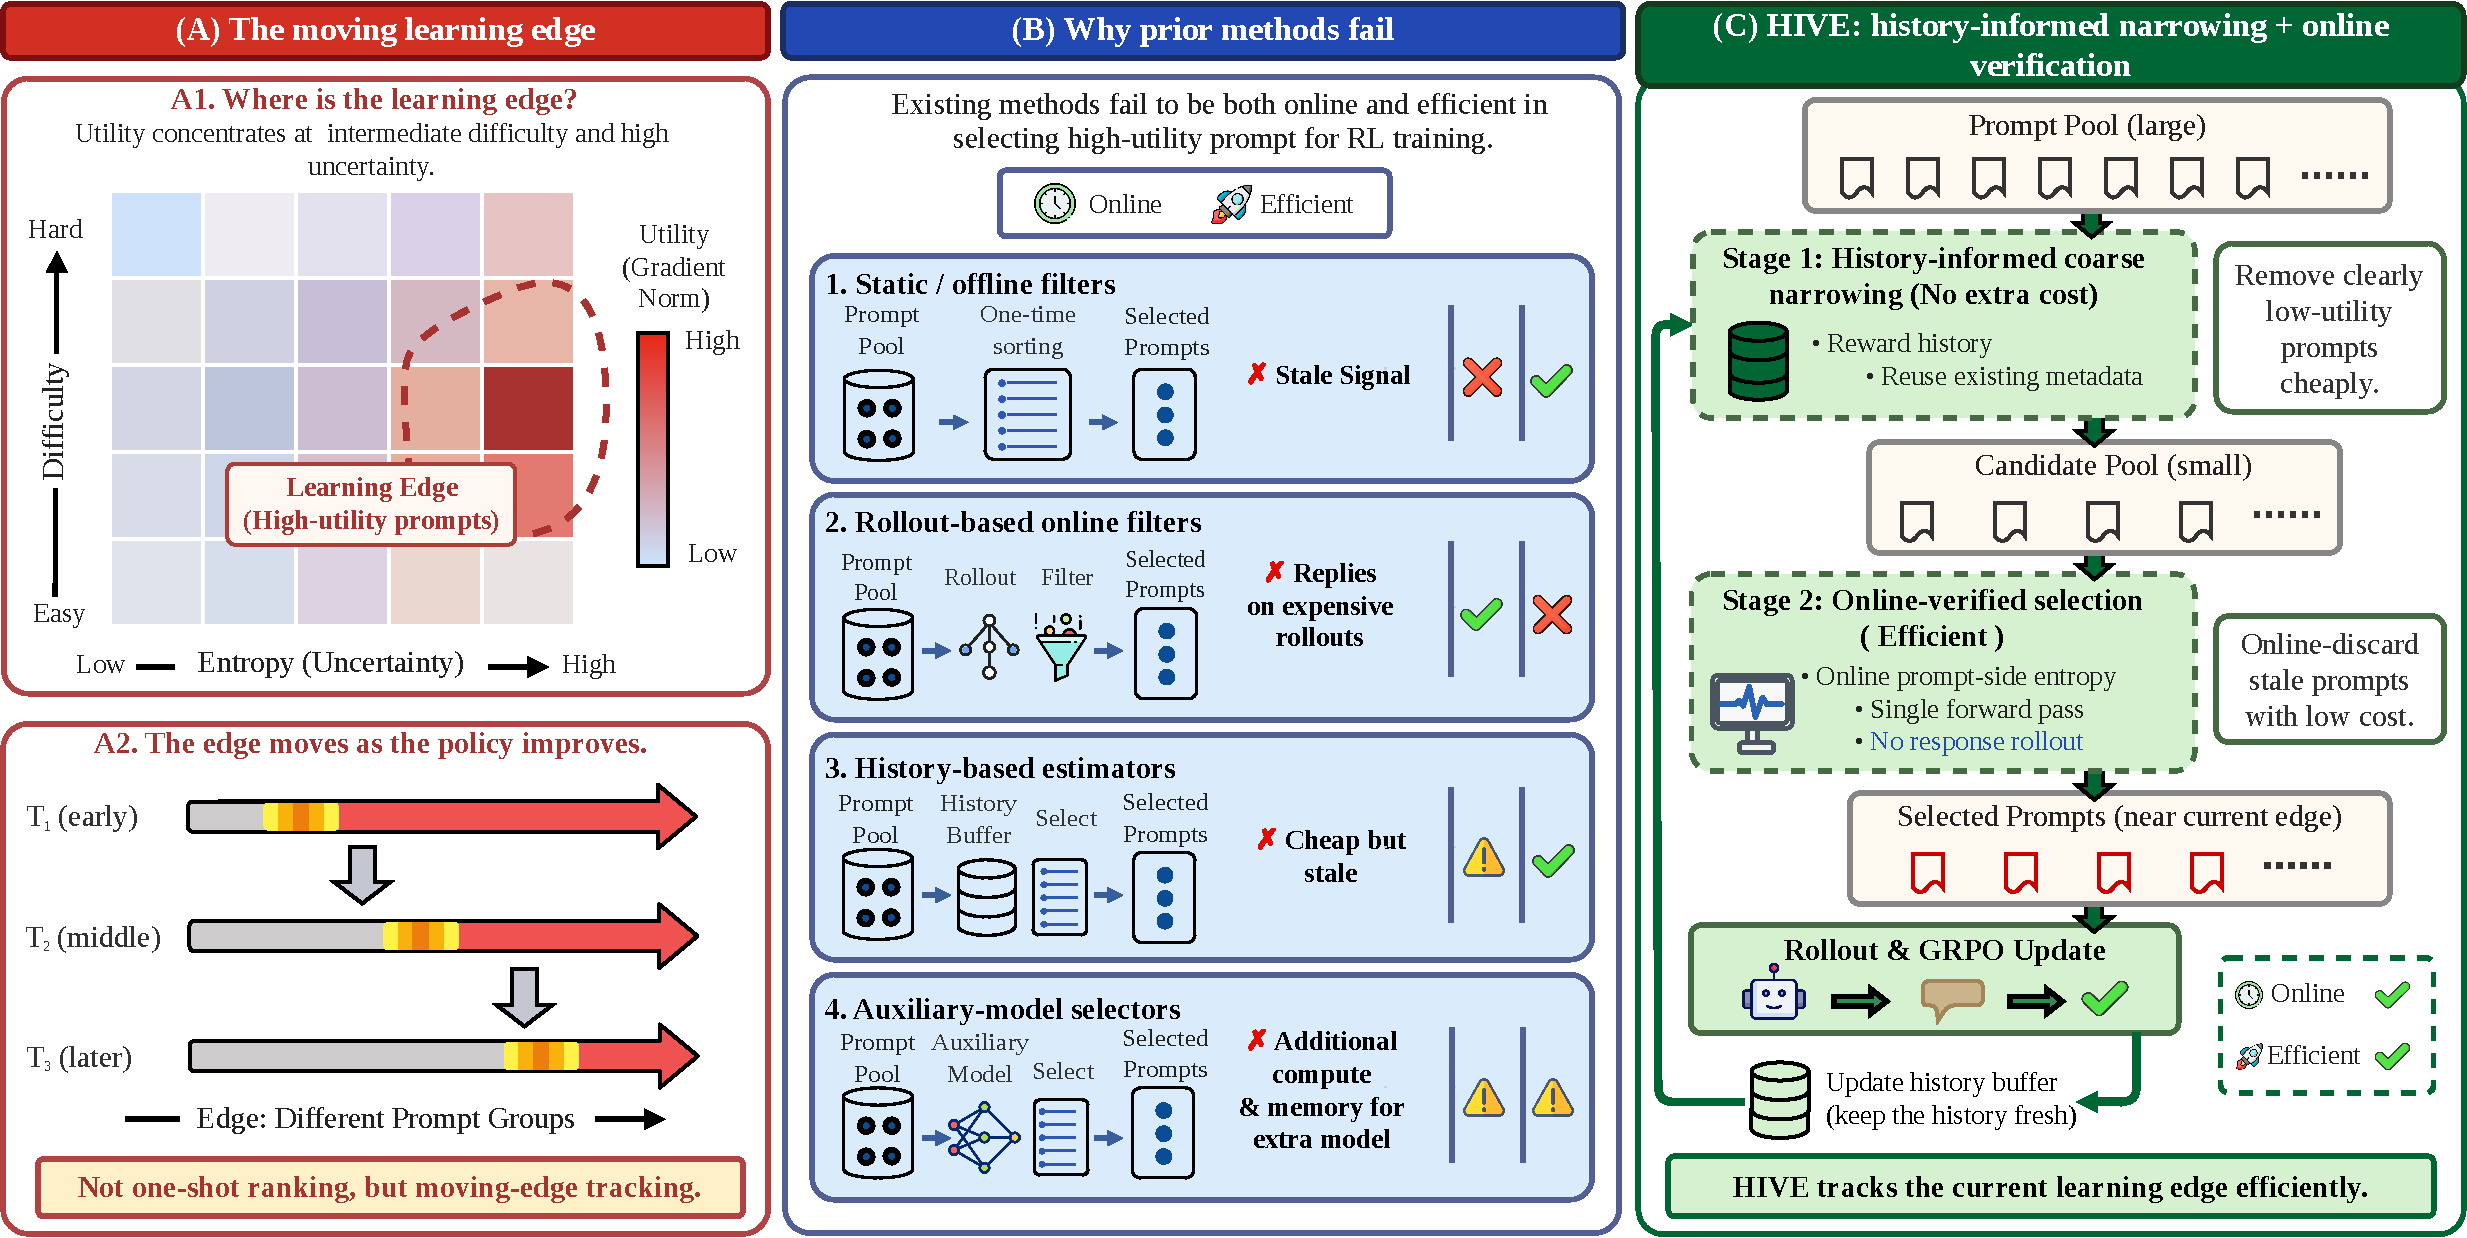
\includegraphics[width=0.98\linewidth]{figures/introduction/intro-fig-compare-motivate-1.pdf}
    \caption{\textbf{RLVR prompt selection is a moving-edge tracking problem.} (A) Utility concentrates at 
    intermediate difficulty and high uncertainty, and the learning edge is dynamic. 
    (B) Prior methods face limitations in efficiently selecting online high-utility prompts. (C) HIVE combines history-informed coarse narrowing with low-cost online 
    verification to track the current learning edge.}
    \label{fig:intro-compare-motivate}
    \vskip -0.2in
\end{figure}
% \red{1. re-write this caption 2.
%     delete precise. 3. redraw figure 3(d) to correspond to the A2 in figure 1. 4. shoud not be like curriculum, 
%     instead the utility of prompts across different step should be varying.}

\section{Introduction}
\label{sec:introduction}
Reinforcement Learning (RL) has emerged as a prevalent paradigm for fine-tuning large language models (LLMs), particularly for enhancing complex mathematical and logical reasoning capabilities~\cite{guo2025deepseek,yu2025dapo,tomihari2026learningdynamicsrlposttraining}. While advanced RL algorithms such as group relative policy optimization (GRPO)~\cite{shao2024deepseekmath} rely on rollout scaling to stabilize training and enhance model performance, they introduce a severe computational overhead~\cite{xu2025not,yu2025dapo,li2026stalefeedbackcoevolvingcritics}. In the training of those RL algorithms, a large portion of computational resources is wasted on generating rollouts for low-utility prompts that are either too trivial or too intractable for the current model. This results in vanishing gradients and wasted resources, providing no informative learning signal for model updates~\cite{zheng2025act,yu2025dapo,noukhovitch2025fasterICLR,verl2025}. Therefore, we investigate the following research question in this paper: \textit{how to identify prompts that are likely to produce useful gradients before rollout?}

Existing methods face limitations in efficiently selecting {high-utility} prompts in an online manner. Static or offline filters rank prompts before training using fixed heuristics, making them inexpensive but unable to adapt to the changing model during RL 
training~\cite{Wang2025ReinforcementLF,Li2025LIMRLI,ye2025limo}. Rollout-based online filters, such as dynamic sampling, better capture the current utility of each prompt by checking reward variance from newly generated responses~\cite{yu2025dapo,xu2025not,Chen2025LSPO,Ye2025PROF}. However, they already incur substantial rollout cost. History-based estimators such as GRESO~\cite{zheng2025act} avoid additional 
rollout cost by estimating prompt utility from past reward statistics, but those metadata becomes stale as the policy 
updates~\cite{zheng2025act,sun2025dots,li2026stalefeedbackcoevolvingcritics}. Auxiliary-model selectors, such as PCL~\cite{Gao2025PCL}, attach external or jointly trained predictors to estimate prompt difficulty or utility, introducing extra compute and memory during selection. 

% To understand what makes a prompt useful during RL training, we first conduct an empirical analysis of GRPO 
% training dynamics.  
% Among prompts with non-zero gradients, high response-side entropy prompts yield stronger learning progress at the same 
% rollout budget (Figure~\ref{fig:intro-a-b}b). More broadly, utility (\red{which we measured via length-normalized gradient norm}) concentrates at the intersection 
% of \red{intermediate difficulty} and high response-side entropy (Figure~\ref{fig:intro-a-b}c), which we term as 
% {learning edge}. However, the edge moves: prompts selected by those historical metadata quickly 
% lose real-time utility, whereas prompts verified under the current policy retain higher gradient norms 
% (Figure~\ref{fig:intro-a-b}a,\ref{fig:intro-a-b}d). Based on these observations, we conclude that an ideal prompt selection 
% framework for efficient LLM RL must be: \textbf{online} to track the moving learning edge, and \textbf{efficient} to avoid excessive overhead for selection.
% To identify what makes a prompt useful during RL training, we first empirically analyze GRPO training dynamics. Among prompts with non-zero gradients, those with high response-side entropy produce greater learning progress under the same rollout budget (Figure~\ref{fig:intro-a-b}b). More broadly, utility, measured by the length-normalized gradient norm, concentrates at the intersection of intermediate difficulty and high response-side entropy (Figure~\ref{fig:intro-a-b}c), which we refer to as the learning edge. However, this edge is dynamic: prompts selected using historical metadata quickly lose real-time utility, whereas prompts verified under the current policy retain higher gradient norms (Figure~\ref{fig:intro-a-b}a,\ref{fig:intro-a-b}d). These observations suggest that an effective prompt selection framework for efficient LLM RL should be \textbf{online}, to track the moving learning edge, and \textbf{efficient}, to avoid excessive selection overhead.
To identify what makes a prompt useful during RL training, we first empirically analyze GRPO training dynamics. Among prompts with non-zero gradients, those with high response-side entropy produce greater learning progress under the same rollout budget (Figure~\ref{fig:intro-high-entropy}). More broadly, utility, measured by the length-normalized gradient norm, concentrates at the intersection of intermediate difficulty and high response-side entropy (Figure~\ref{fig:intro-learning-edge}), which we refer to as the learning edge. However, this edge is dynamic: prompts selected using historical metadata quickly lose real-time utility, whereas prompts verified under the current policy retain higher gradient norms (Figures~\ref{fig:intro-history-staleness}); prompts move substantially among High, Low, and Zero utility classes across training steps (Figure~\ref{fig:intro-utility-shift}). These observations suggest that an effective prompt selection framework for efficient LLM RL should be \textbf{online}, to track the moving learning edge, and \textbf{efficient}, to avoid excessive selection overhead.
% To identify what makes a prompt useful during RL training, we first empirically analyze GRPO training dynamics. Among prompts with non-zero gradients, those with high response-side entropy produce greater learning progress under the same rollout budget (Figure~\ref{fig:intro-high-entropy}). More broadly, utility, measured by the length-normalized gradient norm, concentrates at the intersection of intermediate difficulty and high response-side entropy (Figure~\ref{fig:intro-learning-edge}), which we refer to as the learning edge. However, this edge is dynamic: prompts selected using historical metadata quickly lose real-time utility, whereas prompts verified under the current policy retain higher gradient norms (Figure~\ref{fig:intro-history-staleness}); prompts also move substantially among High, Low, and Zero utility classes across training steps (Figure~\ref{fig:intro-utility-shift}). These observations suggest that an effective prompt selection framework for efficient LLM RL should be \textbf{online}, to track the moving learning edge, and \textbf{efficient}, to avoid excessive selection overhead.


% To understand what makes a prompt useful for RL training, we first empirically examine GRPO training dynamics. Among prompts with non-zero gradients, those with higher response-side entropy yield greater learning progress under the same rollout budget (Figure~\ref{fig:intro-high-entropy}). More generally, utility, measured by the length-normalized gradient norm, is concentrated where intermediate difficulty and high response-side entropy intersect (Figure~\ref{fig:intro-learning-edge}); we refer to this region as the \emph{learning edge}. However, this edge shifts over time: prompts selected using historical metadata rapidly lose real-time utility, whereas prompts verified under the current policy maintain higher gradient norms (Figure~\ref{fig:intro-history-staleness}). Moreover, prompts frequently transition among High-, Low-, and Zero-utility classes throughout training (Figure~\ref{fig:intro-utility-shift}). These findings suggest that an effective prompt selection framework for efficient LLM RL should be both \textbf{online}, to track the moving learning edge, and \textbf{efficient}, to minimize selection overhead.

Based on previous analysis, we propose \textbf{HIVE} (\textbf{H}istory-\textbf{I}nformed \textbf{V}erification of the learning \textbf{E}dge), a dual-stage 
framework for rollout-efficient RLVR (Figure~\ref{fig:framework}). HIVE first performs history-informed coarse narrowing using 
reward trajectories and response-side entropies accumulated from previous training steps. This stage targets efficiency by retaining exploration probability for prompts that are around the edge. HIVE then utilizes prompt entropy as a high-fidelity and efficient proxy to perform online verification under the current policy, filtering stale candidates before the rollout phase.
% HIVE then performs online verification with prompt-side entropy 
% computed under the current policy. This stage restores online precision and filters 
% stale candidates before the rollout phase.

% Evaluation for HIVE is conducted across multiple reasoning benchmarks (e.g., {math, coding, and tool calling}) and models: Qwen3-4B~\cite{yang2025qwen3technicalreport}, 
Evaluation for HIVE is conducted across multiple reasoning benchmarks (e.g., math and tool calling) and models: Qwen3-4B-Base~\cite{yang2025qwen3technicalreport}, 
Qwen2.5-Math-1.5B/7B~\cite{yang2024qwen25mathtechnicalreportmathematical}, DeepSeek-R1-Distill-Qwen-1.5B~\cite{guo2025deepseek}, 
% Qwen2.5-14B/32B~\cite{qwen2.5-large}, and Llama-3.2-3B-Instruct~\cite{grattafiori2024llama3}. HIVE maintains comparable or better accuracy than Dynamic Sampling~\cite{yu2025dapo}, Pre-filter, GRESO~\cite{zheng2025act}, and PCL~\cite{Gao2025PCL} while using fewer rollouts, achieving up to \textbf{3.8$\times$ speedup in rollout} and \textbf{2.3$\times$ faster total training time} for models like Qwen2.5-Math-7B. Finally, we show that HIVE drastically lowers computational overhead, reducing rollouts by \textbf{up to 9.2 million} while consistently maintaining or even exceeding the reasoning accuracy of strong selection baselines across DAPO+MATH, Open-R1, and larger Qwen2.5 model scales.
Qwen2.5-14B/32B~\cite{qwen2.5-large}, and Llama-3.2-3B-Instruct~\cite{grattafiori2024llama3}. HIVE significantly outperforms 
baselines like Dynamic Sampling~\cite{yu2025dapo}, GRESO~\cite{zheng2025act} and PCL~\cite{Gao2025PCL}, achieving up to \textbf{2.3$\times$ faster total training time} for models like Qwen2.5-Math-7B. Finally, we show that HIVE lowers computational 
overhead, achieving \textbf{up to 9.2 million rollouts reduction} while consistently maintaining the reasoning performance. Beyond mathematical reasoning, HIVE also attains the best BFCL-V2 tool-calling score while using \textbf{4.8$\times$ fewer rollouts} than Dynamic Sampling, suggesting that moving-edge tracking extends to verifiable tool-use tasks.
%Besides, \red{the studies on coding and tool-calling tasks also show the generality of HIVE beyond math reasoning.}
% Our contributions are threefold:
% \begin{itemize}[topsep=2pt,itemsep=1pt,leftmargin=*]
%     and efficient required for practical selection. 
%     \item We propose HIVE, a dual-stage selector that combines zero-cost history-informed narrowing with low-cost online verification. 
%     \item We demonstrate across multiple tasks and model scales that HIVE significantly reduces rollout and wall-clock training costs while 
%     preserving or improving performance on those tasks.
% \end{itemize}
\section{Empirical Observations: The Moving Learning Edge}
\label{sec:obs-preliminary}
This section dissects the training dynamics of GRPO-style RLVR to identify what makes a 
prompt useful for policy optimization and why effective selection in RLVR is an online tracking problem. 
We first recall why low-utility prompts produce no GRPO learning signal, then show that the useful 
prompts concentrate at a moving edge characterized by intermediate difficulty and high uncertainty. {The experimental details are reported in Appendix~\ref{sec:preliminary-setup}.}

% \red{The detailed experimental setting is described in Appendix~\ref{appendix:preliminary-experiment-setting}}.
% \red{till here}
% \begin{figure}[t]
%     \centering
%     % Four independent panels, each generated by its own Python script
%     % under unified style (see ICML2026-submission-figure-script-drawio-todo/wandb-figure/).
%     \begin{minipage}[t]{0.245\linewidth}
%         \centering
%         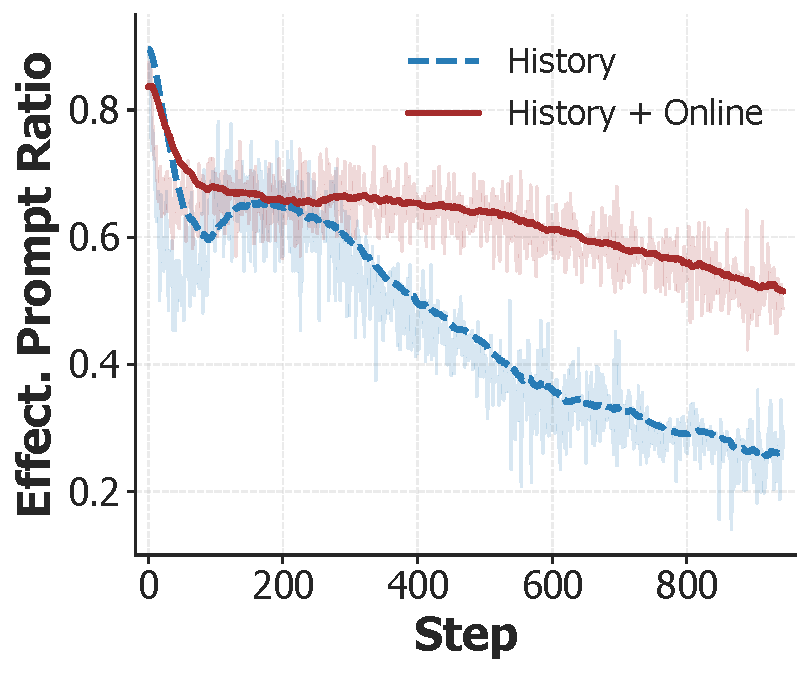
\includegraphics[width=\linewidth]{figures/intro/intro_a_eff_ratio.pdf}
%         \\[-2pt]{\footnotesize\textbf{(a)}\par}
%     \end{minipage}\hfill
%     \begin{minipage}[t]{0.245\linewidth}
%         \centering
%         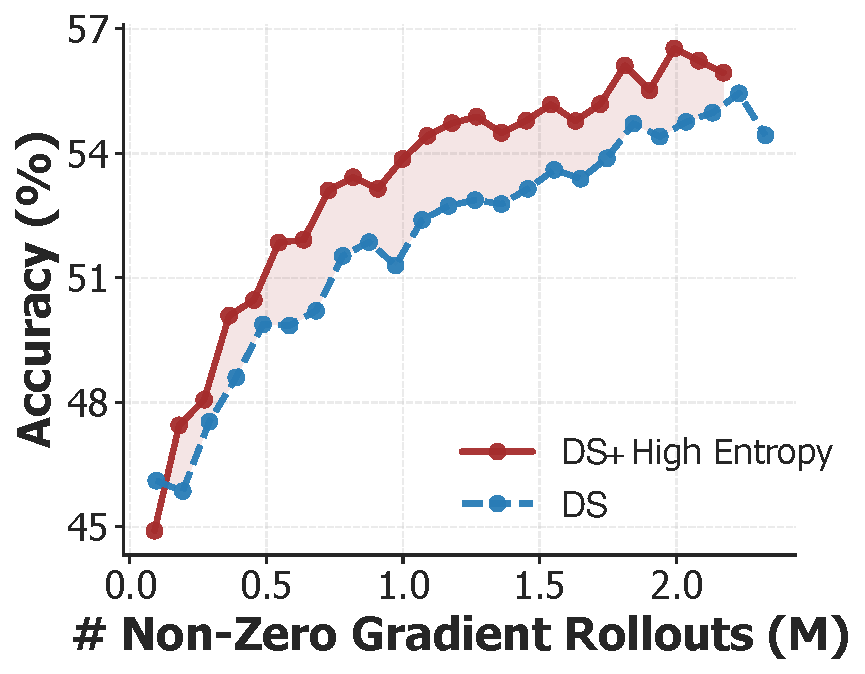
\includegraphics[width=\linewidth]{figures/intro/intro_b_high_entropy-backup.pdf}
%         \\[-2pt]{\footnotesize\textbf{(b)}\par}
%     \end{minipage}\hfill
%     \begin{minipage}[t]{0.245\linewidth}
%         \centering
%         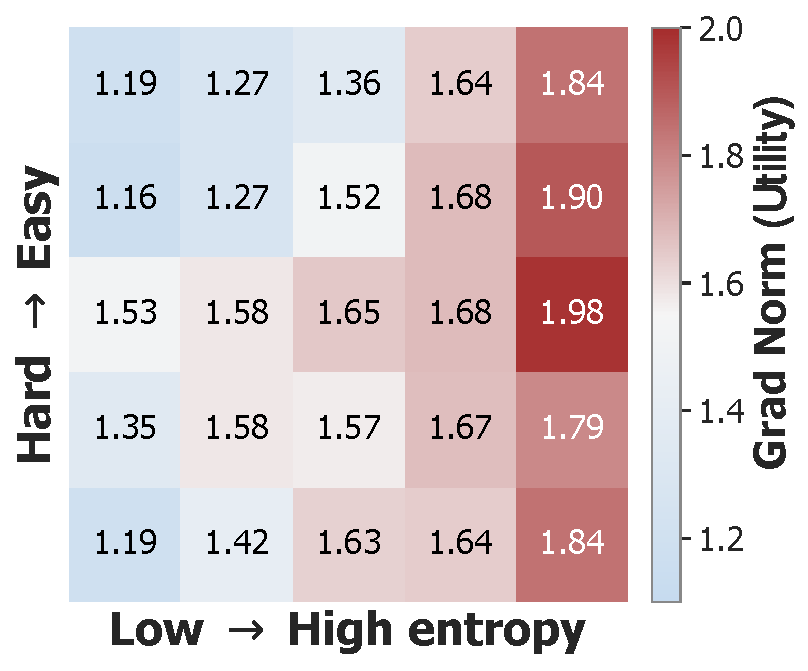
\includegraphics[width=\linewidth]{figures/intro/intro_c_heatmap-backup.pdf}
%         \\[-2pt]{\footnotesize\textbf{(c)}\par}
%     \end{minipage}\hfill
%     \begin{minipage}[t]{0.245\linewidth}
%         \centering
%         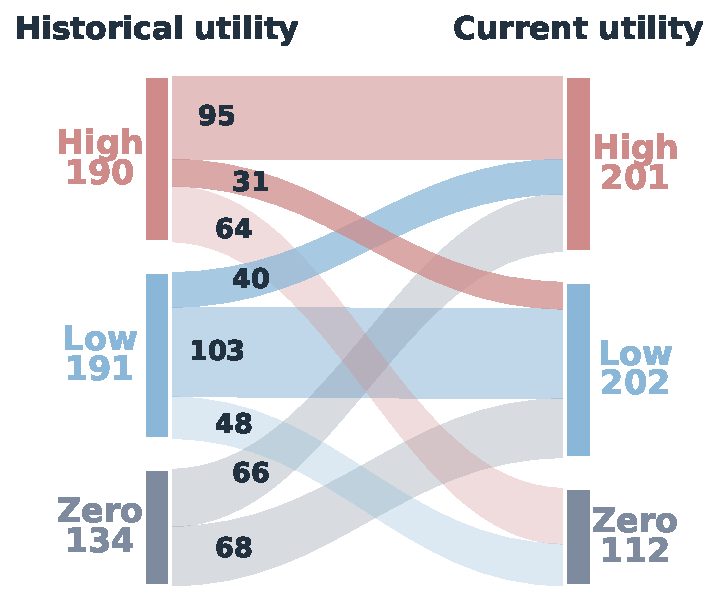
\includegraphics[width=\linewidth]{figures/intro/intro_d_sankey.pdf}
%         \\[-2pt]{\footnotesize\textbf{(d)}\par}
%     \end{minipage}
%     \caption{\textbf{Four empirical observations motivating HIVE.}
%     (a) Selection only based on historical statistics becomes increasingly stale during training, while online verification retains more effective prompts.
%     (b) Among prompts with non-zero gradients, prioritizing high-entropy
%         prompts improves accuracy at the same rollout budget.
%     (c) Gradient utility concentrates at an intermediate-difficulty,
%         high-entropy learning edge.
%     (d) Across two checkpoints (steps 500 and 1000), a large fraction of sampled
%         prompts shift between High, Low, and Zero utility classes, so
%         prompts selected by historical metadata no longer match the
%         current policy's utility distribution. \red{(1) need to re-write the corresponding prelimiary analysis and (2) revise the reference of these four subfigures.}
%     }
%     \label{fig:intro-a-b}
%     \vskip -0.15in
% \end{figure}
\begin{figure}[t]
    \centering
    \captionsetup[subfigure]{labelformat=parens,labelsep=none,font=footnotesize,justification=centering}
    % Four independent panels, each generated by its own Python script
    % under unified style (see ICML2026-submission-figure-script-drawio-todo/wandb-figure/).
    \begin{subfigure}[t]{0.241\linewidth}
        \centering
        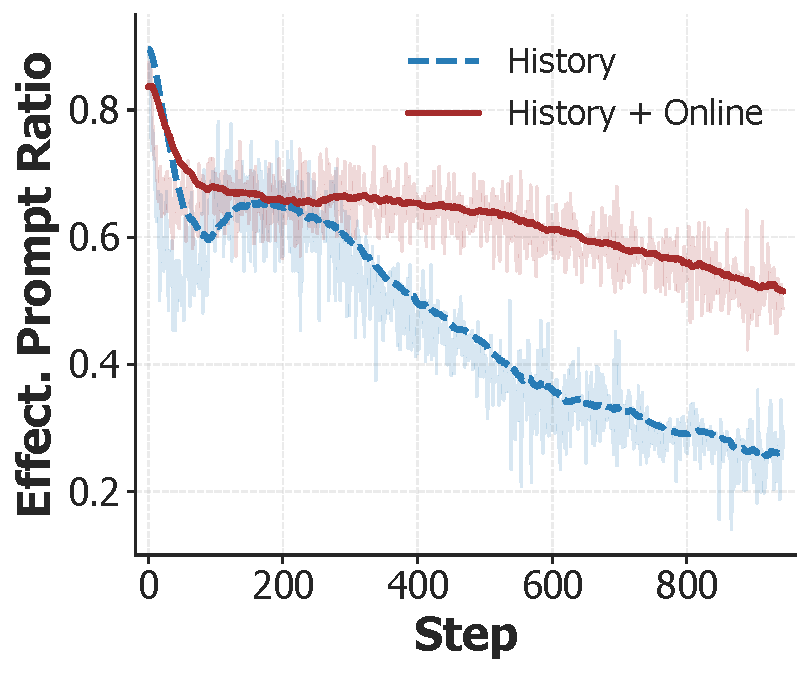
\includegraphics[width=\linewidth]{figures/intro/intro_a_eff_ratio.pdf}
        \vspace{-6pt}
        \caption{}
        \label{fig:intro-history-staleness}
    \end{subfigure}\hfill
    \begin{subfigure}[t]{0.245\linewidth}
        \centering
        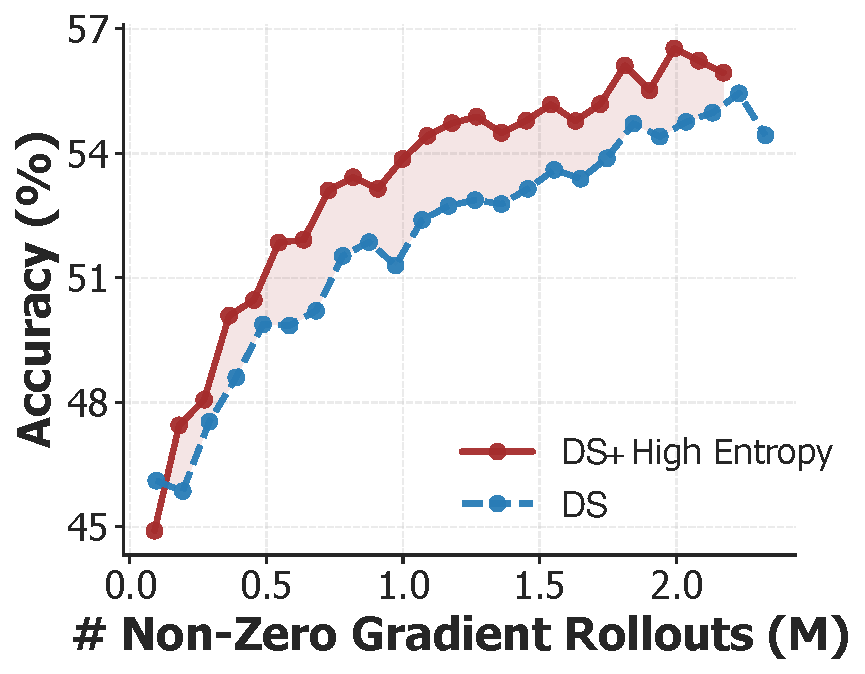
\includegraphics[width=\linewidth]{figures/intro/intro_b_high_entropy-backup.pdf}
        \vspace{-6pt}
        \caption{}
        \label{fig:intro-high-entropy}
    \end{subfigure}\hfill
    \begin{subfigure}[t]{0.245\linewidth}
        \centering
        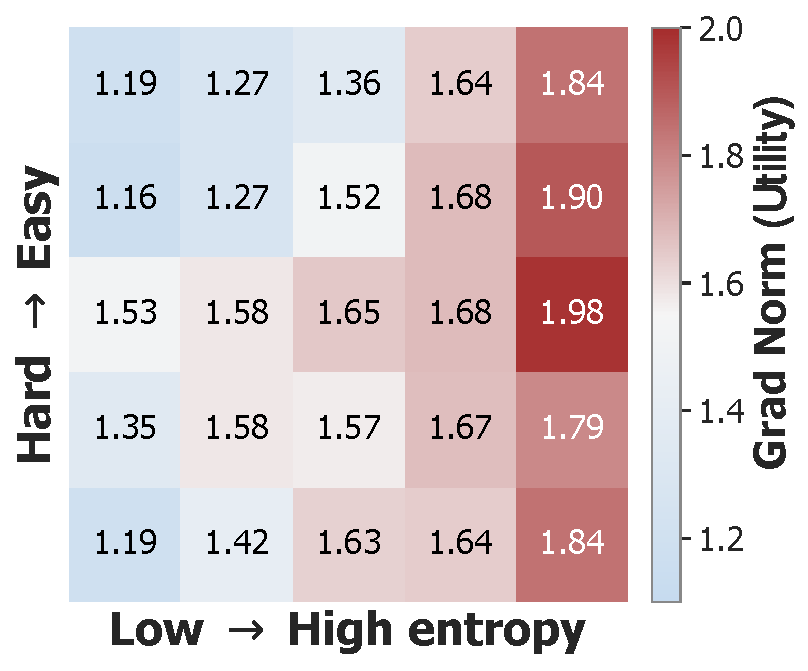
\includegraphics[width=\linewidth]{figures/intro/intro_c_heatmap-backup.pdf}
        \vspace{-6pt}
        \caption{}
        \label{fig:intro-learning-edge}
    \end{subfigure}\hfill
    \begin{subfigure}[t]{0.241\linewidth}
        \centering
        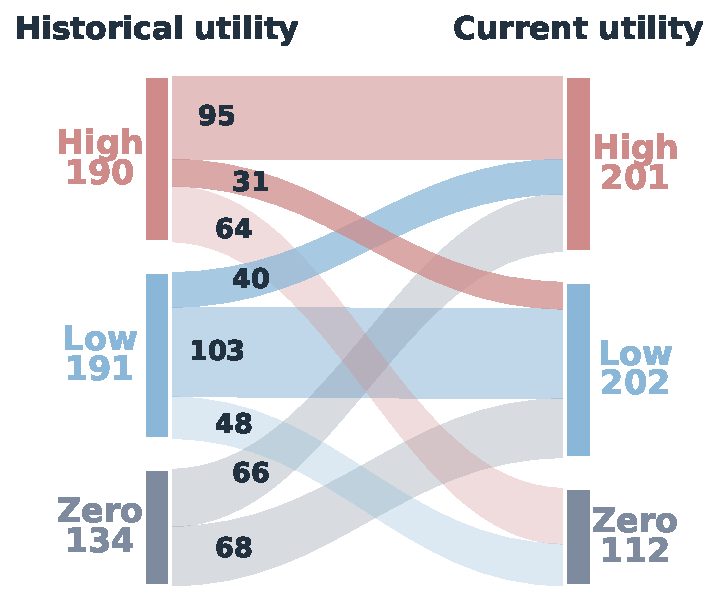
\includegraphics[width=\linewidth]{figures/intro/intro_d_sankey.pdf}
        \vspace{-6pt}
        \caption{}
        \label{fig:intro-utility-shift}
    \end{subfigure}
    \caption{\textbf{Empirical observations.}
    (a) Selection only based on historical statistics becomes increasingly stale during training, while online verification retains more effective prompts.
    (b) Among prompts with non-zero gradients, prioritizing high-entropy
        prompts improves accuracy at the same rollout budget.
    (c) Gradient utility concentrates at an intermediate-difficulty,
        high-entropy learning edge.
    (d) Across two checkpoints (steps 500 and 1000), a large fraction of sampled
        prompts shift between High, Low, and Zero utility classes, so
        prompts selected by historical metadata no longer match the
        current policy's utility distribution.
    }
    \label{fig:intro-a-b}
    \vskip -0.15in
\end{figure}

\begin{figure}[t]
    \centering
    % \includegraphics[width=1.0\linewidth]{figures/icml2026-framework-7.png}
    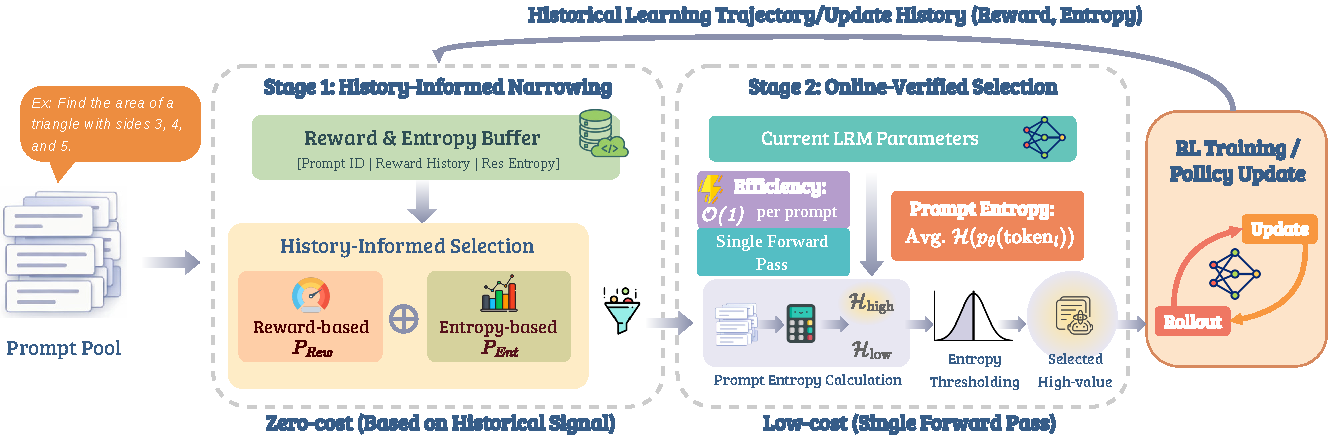
\includegraphics[width=1.0\linewidth]{figures/icml2026-framework-8-compressed.pdf}
    \caption{Overview of HIVE. \textbf{HIVE tracks the moving learning edge by decomposing prompt selection into two stages.}
    \textbf{Stage 1} uses historical reward trajectories and response-side entropy for efficient coarse narrowing. \textbf{Stage 2} computes prompt-side entropy under the current policy for low-cost online verification, rejecting stale candidates before rollout.}
    \label{fig:framework}
    \vskip -0.2in
\end{figure}


\textbf{Zero-variance prompts produce vanishing advantages.}
Group relative policy optimization (GRPO)~\cite{shao2024deepseekmath} is widely used in RLVR for reasoning models~\cite{guo2025deepseek,yang2025qwen3technicalreport}. For a prompt $q$, GRPO samples a group of responses $\{o_i\}_{i=1}^G$ and optimizes
% \begin{equation}
% \label{eq:grpo}
% \begin{aligned}
% \mathcal{J}_{\mathrm{GRPO}}(\theta)
% =
% \mathbb{E}_{\substack{
% q \sim P(Q), \{o_i\}_{i=1}^G \sim \pi_{\theta_{\mathrm{old}}}(\cdot \mid q)
% }}
% \Bigg[
% \frac{1}{G}\sum_{i=1}^G \frac{1}{|o_i|}
% \sum_{t=1}^{|o_i|} \Bigg(
% \min \left(\rho_{i,t}(\theta) \hat{A}_{i, t},&\\
%  \operatorname{clip}(\rho_{i,t}, 1 \pm \varepsilon) \hat{A}_{i, t}\right)
% - \beta D_{\mathrm{KL}}(\pi_\theta \,\|\, \pi_{\mathrm{ref}})
% \Bigg)
% \Bigg].&
% \end{aligned}
% \end{equation}
\begin{equation}
\label{eq:grpo}
\begin{aligned}
\mathcal{J}_{\mathrm{GRPO}}(\theta)
&=
\mathbb{E}_{\substack{
q \sim P(Q),\ \{o_i\}_{i=1}^{G} \sim \pi_{\theta_{\mathrm{old}}}(\cdot \mid q)
}}
\Biggl\{
\frac{1}{G}\sum_{i=1}^{G}\frac{1}{|o_i|}
\sum_{t=1}^{|o_i|}
\biggl(
\min \Bigl[
\frac{\pi_{\theta}(o_{i,t}\mid q,o_{i,<t})}{\pi_{\theta_{\mathrm{old}}}(o_{i,t}\mid q,o_{i,<t})}\hat{A}_{i,t}, \\
&\qquad\qquad\;
\operatorname{clip}(
\frac{\pi_{\theta}(o_{i,t}\mid q,o_{i,<t})}{\pi_{\theta_{\mathrm{old}}}(o_{i,t}\mid q,o_{i,<t})}, 1-\varepsilon, 1+\varepsilon
)\hat{A}_{i,t}
\Bigr]
-\beta D_{\mathrm{KL}}\!\left[
\pi_{\theta}\,\|\,\pi_{\mathrm{ref}}
\right]
\biggr)
\Biggr\},
\end{aligned}
\end{equation}
% where
% \begin{equation}
%     \mathcal{L}^{\mathrm{clip}}_{i,t}(\theta)=\min \left(\rho_{i,t}(\theta) \hat{A}_{i, t}, \operatorname{clip}(\rho_{i,t}, 1 \pm \varepsilon) \hat{A}_{i, t}\right).
% \end{equation}
% where the group-normalized advantage $\hat{A}_{i}$ is computed as follows\red{ need more justifications on the notations}:
where $P(Q)$ is the prompt distribution, $G$ is the response group size, and $o_{i,t}$ denotes the $t$-th token
of response $o_i$. The KL penalty with weight $\beta$ anchors $\pi_\theta$ to the
reference policy $\pi_{\mathrm{ref}}$. Since RLVR gives a sequence-level reward $r_i$, all tokens in $o_i$
share the group-normalized advantage $\hat{A}_{i,t}=\hat{A}_{i}$:
\begin{equation}
\label{eq:grpo_advantage}
\hat{A}_{i} = \frac{r_i - \mathrm{mean}(\{r_i\}_{i=1}^G)}{\mathrm{std}(\{r_i\}_{i=1}^G)}.
\end{equation}
When all sampled responses for a prompt receive the same reward, the reward variance is zero and the prompt contributes no informative policy-gradient signal. Such prompts are either already easy for the current policy or still too hard to discriminate among sampled responses. Rollout scaling therefore wastes compute unless it avoids these zero-variance regions.

\textbf{Utility concentrates at an intermediate-difficulty, high-entropy edge.}
Zero-variance filtering is necessary but not sufficient: among prompts with non-zero gradients, some still provide much stronger learning signal than others. Following previous analyses~\cite{kim2025mitigatinglengthbiasrlhf,paul2021DataDiet,fayyaz2022bertdatadietfinding,singhal2024aCOLM}, we use length-normalized gradient norm as a proxy for per-prompt utility and study how it varies with empirical difficulty and response-side entropy.

Figure~\ref{fig:intro-learning-edge} shows two consistent patterns. First, within a fixed difficulty band, gradient norm increases with response-side entropy. Second, at a fixed entropy level, utility follows an inverted-U shape over 
difficulty: trivial prompts and intractable prompts have low utility, while intermediate-difficulty prompts have 
higher utility. The strongest learning signal appears at the intersection of these two conditions. We call this 
region the \textit{learning edge}. This observation explains why merely removing zero-variance prompts is too 
coarse: \textit{the best rollout budget should be allocated to prompts that are both learnable and uncertain under the 
current policy}.

\textbf{Historical metadata becomes stale as the edge moves.}
As the policy updates, the model's state of knowledge changes, and historical 
metadata such as reward trajectories and response entropies can quickly become stale~\cite{cui2025entropymechanismreinforcementlearning,tomihari2026learningdynamicsrlposttraining,li2026stalefeedbackcoevolvingcritics}. 
To quantify this effect, we compare prompts selected by historical metadata from the previous training window 
with prompts selected by online metrics recomputed under the current policy. As shown in Figure~\ref{fig:intro-utility-shift}, 
historical selection yields lower current gradient norms, whereas online selection isolates prompts with high utility. Figure~\ref{fig:intro-utility-shift} further shows that prompts frequently move among High, Low, and Zero utility classes across training steps. Together, these results indicate that: \textit{a selector must revalidate candidate prompts under the current policy to keep tracking the moving edge}.

\section{Methodology}
\label{sec:method}
\begingroup
\setlength{\abovedisplayskip}{5pt plus 1pt minus 1pt}
\setlength{\belowdisplayskip}{5pt plus 1pt minus 1pt}
\setlength{\abovedisplayshortskip}{3pt plus 1pt minus 1pt}
\setlength{\belowdisplayshortskip}{3pt plus 1pt minus 1pt}
Section~\ref{sec:obs-preliminary} shows that useful RLVR prompts concentrate near a moving learning edge and historical metadata alone is unreliable because the edge moves as the policy changes. Bbased on these observations, HIVE is designed as a two-stage pre-rollout selector (Figure~\ref{fig:framework} and Algorithm~\ref{alg:hive-training}). Stage~1 uses historical reward and response-entropy traces as a cheap prior to form a candidate pool; Stage~2 revalidates those candidates under the current policy using prompt-side entropy before expensive rollouts for the standard GRPO update.

\subsection{Design Objective}
A practical RLVR prompt selector must be both \textbf{online}, adapting as the policy evolves and the learning frontier shifts during training, and \textbf{efficient}, avoiding full response rollouts that could erase its computational benefits. HIVE achieves this via two stages. Stage~1 targets efficiency: it uses historical reward trajectories and response-side entropies to cheaply narrow the full prompt pool to a candidate set. Stage~2 restores online precision: it verifies candidates with prompt-side entropy computed under the current model parameters. The final selected prompts are then passed to the standard rollout and GRPO update. The detailed procedure is provided in Appendix~\ref{appendix-sec:alg}.

\subsection{Stage 1: History-Informed Coarse Narrowing}
Stage~1 removes prompts that are unlikely to lie near the learning edge while keeping enough exploration to handle edge movement. It combines a reward-based score, which tracks difficulty saturation, with an entropy-based score, which favors historically uncertain prompts.

% \textbf{Reward-based score.}
% For each prompt $x_i\in \mathcal{D}$, HIVE maintains a historical trace
% \begin{equation}
%     T_i = \{R_{i,1},\ldots,R_{i,n}\},
% \end{equation}
% where $R_{i,j}=\{r_{i,j}^{(k)}\}_{k=1}^G$ is the reward group obtained from $G$ rollouts at the $j$-th recorded iteration. Let $\mathbb{I}_{i,j}=1$ if all rewards in $R_{i,j}$ are identical, and $0$ otherwise. We define the most recent consecutive zero-variance count as
% % \begin{equation}
%     $z_i = \max \left\{ k \in [0,n] \mid \prod_{j=n-k+1}^{n} \mathbb{I}_{i,j} = 1 \right\}.$
% % \end{equation}
% The reward-based retention probability is:
% \begin{equation}
%     P_{\mathrm{Rew}}(x_i)=p_e^{z_i},
% \end{equation}
% where $p_e\in(0,1)$ is a base exploration probability. Prompts that repeatedly produce identical rewards are retained with decreasing probability, but never deterministically removed; this matters because hard prompts can become learnable later as the policy improves.

% HIVE adjusts $p_e$ online to avoid manual tuning across models and stages. At each iteration, it compares the observed zero-variance ratio with a target $\alpha$ and updates $p_e$ by a step size $\Delta p$: if too many selected prompts are zero-variance, $p_e$ is decreased; otherwise, it is increased. We maintain separate probabilities $p_{e,\mathrm{easy}}$ and $p_{e,\mathrm{hard}}$ for all-correct and all-incorrect zero-variance prompts, allowing HIVE to control over-sampling of mastered and intractable regions independently.

% \textbf{Entropy-based score.}
% Historical response-side entropy provides a low-cost prior over uncertainty. For the most recent rollout group of prompt $x_i$, define
% \begin{equation}
%     H_i = \frac{1}{G} \sum_{r=1}^{G} U^{(r)}(x_i),\quad
%     U^{(r)}(x_i) = \frac{1}{L_r} \sum_{l=1}^{L_r} \mathcal{H}(p^{(r)}_{\theta,l}),
% \end{equation}
% where $p^{(r)}_{\theta,l}$ is the token distribution at response position $l$ in rollout $r$, $L_r$ is the response length, and
% \begin{equation}
%     \mathcal{H}(p_{\theta}(\cdot | c)) = - \sum_{v \in \mathcal{V}} p_{\theta}(v | c) \log p_{\theta}(v | c).
% \end{equation}
% We normalize $H_i$ within the current metadata pool:
% \begin{equation}
%     P_{\mathrm{Ent}}(x_i)=\frac{H_i-H_{\min}}{H_{\max}-H_{\min}+\epsilon},
% \end{equation}
% where $\epsilon$ is a small constant for numerical stability.

% \textbf{Candidate sampling.}
% The Stage~1 selection probability combines difficulty saturation and uncertainty:
% \begin{equation}
%     P_{\mathrm{select}}(x_i) = \lambda P_{\mathrm{Rew}}(x_i)+(1-\lambda)P_{\mathrm{Ent}}(x_i),
% \end{equation}
% where $\lambda$ balances reward-history pruning and entropy-based prioritization. Stage~1 samples candidates according to $P_{\mathrm{select}}$ until the candidate pool is large enough for Stage~2 verification. This coarse narrowing is effectively zero-cost because it reuses metadata already produced by previous training iterations.
\textbf{Reward-history score.}
For each prompt $x_i\in\mathcal{D}$, HIVE stores a trace $\mathcal{T}_i^{(t)}=\{R_{i,j}\}_{j=1}^{n_i}$ before training step $t$, where $R_{i,j}=\{r_{i,j}^{(k)}\}_{k=1}^{G}$ is the reward group recorded at the $j$-th previous visit. Let $\zeta_{i,j}=\mathbf{1}\{\operatorname{Var}(R_{i,j})=0\}$ indicate whether that visit produced a zero-variance reward group. HIVE summarizes recent saturation by the length of the trailing zero-variance run:
\begin{equation}
\label{eq:stage1_reward_score}
\begin{aligned}
&z_i^{(t)}
=\max\left\{k\in\{0,\ldots,n_i\}:
\prod_{j=n_i-k+1}^{n_i}\zeta_{i,j}=1\right\},\\
&s_{\mathrm{rew}}(x_i)
=\left(p_{e,\tau_i}^{(t)}\right)^{z_i^{(t)}},
\qquad \tau_i\in\{\mathrm{easy},\mathrm{hard}\}.
\end{aligned}
\end{equation}
Here $\tau_i$ distinguishes all-correct and all-incorrect zero-variance prompts, and $p_{e,\tau_i}^{(t)}\in(0,1)$ is the corresponding exploration probability. Repeated zero-variance outcomes therefore decay the retention score exponentially, but do not deterministically discard the prompt. This is important because an intractable prompt may later become learnable as the policy improves.

HIVE adapts the easy and hard exploration probabilities online. If the observed zero-variance ratio $\hat{\rho}_{\tau}^{(t)}$ for type $\tau$ exceeds the target $\alpha$, HIVE decreases $p_{e,\tau}$; otherwise, it increases it:
\begin{equation}
\label{eq:adaptive_pe}
p_{e,\tau}^{(t+1)}
=
\left[
p_{e,\tau}^{(t)}
+\Delta p\cdot\operatorname{sign}\!\left(\alpha-\hat{\rho}_{\tau}^{(t)}\right)
\right]_{[p_{\min},p_{\max}]},
\qquad \tau\in\{\mathrm{easy},\mathrm{hard}\},
\end{equation}
where $[\cdot]_{[p_{\min},p_{\max}]}$ denotes projection to a valid probability range. This update prevents HIVE from persistently over-sampling either mastered prompts or currently intractable prompts.

\textbf{Response-entropy score.}
Historical response-side entropy provides a low-cost prior for uncertainty. For the most recent rollout group of $x_i$, let
\begin{equation}
\label{eq:stage1_entropy_score}
\begin{aligned}
&U_i^{(r)}
=\frac{1}{L_{i,r}}\sum_{\ell=1}^{L_{i,r}}
\mathcal{H}\!\left(p_{\theta}(\cdot\mid x_i,o_{i,<\ell}^{(r)})\right),
\qquad
H_i=\frac{1}{G}\sum_{r=1}^{G}U_i^{(r)},\\
&s_{\mathrm{ent}}(x_i)
=\frac{H_i-H_{\min}}{H_{\max}-H_{\min}+\epsilon},
\qquad\;\;
\mathcal{H}(p)=-\sum_{v\in\mathcal{V}}p_v\log p_v .
\end{aligned}
\end{equation}
The normalization is computed within the current metadata pool. It makes the entropy score comparable across training stages even as the policy becomes more confident.

\textbf{Candidate sampling.}
The Stage~1 acceptance probability combines recent reward saturation and historical uncertainty:
\begin{equation}
\label{eq:stage1_select}
P_{\mathrm{S1}}(x_i)
=
\lambda s_{\mathrm{rew}}(x_i)
+(1-\lambda)s_{\mathrm{ent}}(x_i),
\qquad \lambda\in[0,1].
\end{equation}
HIVE samples prompts with Bernoulli probability $P_{\mathrm{S1}}(x_i)$ until it obtains a candidate set $\mathcal{C}_t$ for Stage~2. Since all quantities in Eq.~\eqref{eq:stage1_select} are from existing training metadata, Stage~1 is zero-cost.

\subsection{Stage 2: Online-Verified Selection}
\label{subsec:stage2}
% Stage~1 is efficient, but its metadata becomes stale as model is consistently trained. Stage~2 therefore verifies candidate prompts under the current policy before rollouts are generated. Full online verification through response generation would require $G$ responses per candidate, so HIVE instead uses prompt-side entropy as a lightweight proxy for current uncertainty.
Stage~1 is efficient, but Section~\ref{sec:obs-preliminary} shows why it cannot be the final decision rule: reward and entropy traces become stale as the current policy moves. Stage~2 therefore verifies the candidate set $\mathcal{C}_t$ under the current policy $\pi_{\theta_t}$ before rollouts are generated. Instead of generating $G$ responses per candidate, HIVE uses prompt-side entropy as a lightweight proxy for current uncertainty.

% \textbf{Prompt-side entropy.}
% For a prompt sequence $x=(x_1,\ldots,x_{L_p})$, HIVE computes
% \begin{equation}
%     V(x) \coloneqq \frac{1}{L_p-1} \sum_{l=2}^{L_p} \mathcal{H}(p_{{\theta}}(\cdot | x_{<l})).
% \end{equation}
% This quantity is online because it is evaluated with the current policy parameters, but efficient because it only requires a prompt-side forward pass. We use it as a verifier of whether a historically promising prompt remains uncertain for the current model.

% We provide a rank-consistency justification under simplifying assumptions, rather than treating prompt entropy as a complete theoretical characterization of utility. Under the representation approximation and entropy propagation assumptions stated in Appendix~\ref{subsec:thm-theoretical-proof}, prompt-side entropy preserves the ranking of expected response-side entropy when the prompt-entropy margin is larger than the combined approximation and sampling noise:
% \begin{theorem}[Informal rank consistency]
% \label{thm:ranking-informal}
% For any pair of prompts $(x,x')$, if the difference in their prompt-side entropy is sufficiently large as specified in Appendix~\ref{appendix-sec:proof-thm}, then with high probability
% \begin{equation}
%  \operatorname{sign}(V(x)-V(x')) = \operatorname{sign}(\hat{U}(x)-\hat{U}(x')),
% \end{equation}
% where $\hat{U}$ is the empirical response-side entropy estimator.
% \end{theorem}
% The main role of this result is to explain why prompt-side entropy can serve as a low-cost online verifier. Our empirical evidence, including the prompt--response entropy correlation in Appendix~\ref{appendix-sec:additional-exp} and the ablations in Section~\ref{subsec:exp-component-study}, provides the primary support for using this proxy in HIVE.

% \textbf{Median verification gate.}
% Let $\mathcal{D}_{S1}$ be the candidate set produced by Stage~1 and the final rollout set can be obtained as follows: 
% \begin{equation}
%     \mathcal{D}_{\mathrm{final}} = \{x \in \mathcal{D}_{S1} \mid V(x) \geq \gamma\},\;\text{where}\;\gamma \coloneqq \mathrm{median}\left(\{ V(x) \mid x \in \mathcal{D}_{S1} \}\right).
% \end{equation}
% $\gamma$ is the prompt-side entropy for all candidates and sets an adaptive threshold. The median gate keeps the throughput stable while adapting the threshold to the current candidate pool. It also matches the purpose of Stage~2: reject stale low-uncertainty prompts after history-informed narrowing, without paying for full response-side verification.

% \textbf{Computational cost.}
% For each candidate, Stage~2 requires one prompt-side forward pass over $L_p$ prompt tokens. A rollout-based verifier would require generating $G$ responses of average length $L_r$ before deciding whether to train on the prompt. Since $L_r$ is typically much larger than $L_p$ in reasoning RLVR and generation is the dominant cost, prompt-side verification is negligible relative to multi-rollout filtering. Section~\ref{subsec:further-experiment} empirically confirms this: online verification adds only 0.82 seconds per iteration, less than 0.4\% of the step time.
\textbf{Prompt-side entropy.}
For a prompt $x=(x_1,\ldots,x_{L_x})$, HIVE computes
\begin{equation}
\label{eq:prompt_entropy}
V_t(x)
=
\frac{1}{L_x-1}\sum_{\ell=2}^{L_x}
\mathcal{H}\!\left(p_{\theta_t}(\cdot\mid x_{<\ell})\right).
\end{equation}
This score is online because it is evaluated with the current policy parameters, and efficient because it only requires a prompt-side forward pass. In the HIVE pipeline, this verifier complements Stage~1: reward history filters repeated zero-variance regions, while $V_t(x)$ checks whether a historically promising candidate still exhibits current-policy uncertainty.

We use an informal rank-consistency result to justify prompt entropy as a verifier, rather than as a complete utility model. Under the representation approximation and entropy propagation assumptions stated in Appendix~\ref{subsec:thm-theoretical-proof}, prompt-side entropy preserves the ranking of expected response-side entropy when the prompt-entropy margin is larger than the combined approximation and sampling noise.
\begin{theorem}[Informal rank consistency]
\label{thm:ranking-informal}
For any pair of prompts $(x,x')$, if the difference in their prompt-side entropy is sufficiently larger as specified in Appendix~\ref{appendix-sec:proof-thm}, then with high probability
\begin{equation}
\operatorname{sign}\!\left(V_t(x)-V_t(x')\right)
=
\operatorname{sign}\!\left(\hat{U}_t(x)-\hat{U}_t(x')\right),
\end{equation}
where $\hat{U}_t$ is the empirical response-side entropy estimator under the current policy.
\end{theorem}
The theorem explains why prompt-side entropy can serve as a low-cost online verifier. The main support for using this proxy remains empirical: Appendix~\ref{appendix-sec:additional-exp} reports prompt--response entropy correlations, and Section~\ref{subsec:exp-component-study} shows that removing Stage~2 weakens the accuracy--rollout tradeoff.

\textbf{Median verification gate.}
Given the Stage~1 candidate set $\mathcal{C}_t$, HIVE uses a median gate:
\begin{equation}
\label{eq:median_gate}
\gamma_t=\operatorname{median}\{V_t(x):x\in\mathcal{C}_t\},
\qquad
\mathcal{B}_t=\{x\in\mathcal{C}_t:V_t(x)\ge\gamma_t\}.
\end{equation}
The final set $\mathcal{B}_t$ is the rollout batch for the current GRPO step. The median threshold keeps throughput stable, adapts to the current candidate distribution, and rejects stale low-uncertainty prompts.

\textbf{Computational cost.}
For $|\mathcal{C}_t|$ candidates, Stage~2 costs $\mathcal{O}(|\mathcal{C}_t|)$ times forward computation. A rollout-based verifier would require $\mathcal{O}(|\mathcal{C}_t|GL_r)$ times. Thus prompt-side verification is negligible relative to multi-rollout filtering. Section~\ref{subsec:further-experiment} empirically confirms this: online verification adds only 0.82 seconds per iteration, less than 0.4\% of the step time.
\endgroup

% % 确保在导言区添加：
% % \usepackage{subcaption}
% % \usepackage{booktabs}
% % \usepackage{graphicx}
% % \usepackage{makecell} 

% \begin{table*}[t]
%     \centering
%     % 总标题（可选，如果不需要总标题可以留空或删除）
%     \caption{Comprehensive evaluation of HIVE on math reasoning benchmarks and efficiency analysis. We train four models on DAPO+MATH. (a) HIVE preserves or improves accuracy while reducing the number of rollouts. (b) HIVE lowers rollout cost, achieving up to 3.8$\times$ rollout speedup and 2.3$\times$ total training speedup over Dynamic Sampling.}
%     \label{tab:main_comparison}

%     % --- 左侧表格 (Performance) ---
%     \begin{subtable}{0.66\textwidth}
%         \centering
%         \caption{Performance (\%) comparison across six math reasoning benchmarks.}
%         \label{tab:model_performance} % 独立的 Label
        
%         % 使用 resizebox 确保表格适应 subtable 的宽度
%         \resizebox{\linewidth}{!}{
%             \begin{tabular}{c|cccccc|c|c}
%             \toprule
%             {Method} & {Math500} & {AIME24} & {AMC} & {Gaokao} & {Miner.} & {Olymp.} & {Avg.} & {\#Rollout} \\
%             \midrule
            
%             % Block 1: Qwen2.5-Math-1.5B
%             \multicolumn{9}{c}{{\textit{Qwen2.5-Math-1.5B}}} \\
%             \midrule
%             DS    & 77.3 & 16.7 & 61.7 & 64.2 & 31.8 & 38.7 & 48.4 & 7.6M (1.0$\times$) \\
%             GRESO & 77.3 & 15.0 & 59.3 & 66.2 & 32.6 & 38.5 & 48.1 & 3.3M (2.3$\times$)\\
%             HIVE  & 77.9 & 16.7 & 60.2 & 66.1 & 31.5 & 40.3 & 48.8 & \best{3.1M (2.5$\times$)} \\
%             \midrule
            
%             % Block 2: DeepSeek-R1-Distill-Qwen-1.5B
%             \multicolumn{9}{c}{{\textit{DeepSeek-R1-Distill-Qwen-1.5B}}} \\
%             \midrule
%             DS    & 87.9 & 36.7 & 71.7 & 78.7 & 35.3 & 54.9 & 60.9 & 2.4M (1.0$\times$)\\
%             GRESO & 85.5 & 37.5 & 70.7 & 76.2 & 34.3 & 52.1 & 59.4 & 1.6M (1.5$\times$)\\
%             HIVE  & 87.2 & 37.5 & 70.1 & 77.2 & 35.1 & 53.2 & 60.1 & \best{1.5M (1.6$\times$)} \\
%             \midrule
            
%             % Block 3: Llama3.2-3b-Instruct
%             \multicolumn{9}{c}{{\textit{Llama3.2-3b-Instruct}}} \\
%             \midrule
%             DS    & 52.4 & 16.7 & 46.0 & 49.2 & 20.0 & 20.2 & 34.1 & {11.4M (1.0$\times$)} \\
%             GRESO & 51.8 & 16.7 & 46.3 & 49.4 & 19.7 & 19.6 & 33.9 & 5.9M (1.9$\times$) \\
%             HIVE  & 53.8 & 17.5 & 45.5 & 49.1 & 20.5 & 20.0 & 34.4 & \best{4.8M (2.4$\times$)} \\
%             \midrule
            
%             % Block 4: Qwen2.5-Math-7B
%             \multicolumn{9}{c}{{\textit{Qwen2.5-Math-7B}}} \\
%             \midrule
%             DS    & 82.9 & 34.2 & 79.2 & 71.7 & 35.4 & 43.6 & 57.8 & 13.1M (1.0$\times$)\\
%             GRESO & 93.2 & 30.0 & 78.9 & 70.2 & 35.2 & 44.1 & 58.6 & 6.3M (2.1$\times$)\\
%             HIVE  & 93.0 & 36.7 & 79.2 & 70.8 & 34.8 & 43.8 & 59.7 & \best{3.9M (3.4$\times$)} \\
%             \bottomrule
%             \end{tabular}
%         }
%     \end{subtable}
%     \hfill % 左右表格之间的弹性间距
%     % --- 右侧表格 (Efficiency) ---
%     \begin{subtable}{0.32\textwidth}
%         \centering
%         \caption{Training time (hours).}
%         \label{tab:efficiency_cost} % 独立的 Label
        
%         % 同样使用 resizebox 适应宽度
%         \resizebox{\linewidth}{!}{
%             \begin{tabular}{c|ccc|c}
%             \toprule
%             Method & Train & Other & Rollout & Total \\ % 稍微缩写一下表头以适应窄宽
%             \midrule
            
%             % Block 1: Qwen2.5-Math-1.5B
%             \multicolumn{5}{c}{{\textit{Qwen2.5-Math-1.5B}}} \\
%             \midrule
%             DS    & 10.9 & 6.0 & 77.3 & 94.2 \\
%             GRESO & 11.3 & 6.4 & 46.0 & 63.7 \\
%             HIVE  & 11.2 & 6.2 & \best{42.1} & \best{59.5} \\
%             \midrule
            
%             % Block 2: DeepSeek
%             \multicolumn{5}{c}{{\textit{DeepSeek-R1-Distill-Qwen-1.5B}}} \\
%             \midrule
%             DS    & 9.6  & 6.1 & 68.7 & 84.4 \\
%             GRESO & 10.4 & 6.6 & 45.9 & 62.9 \\
%             HIVE  & 10.1 & 6.7 & \best{42.7} & \best{59.5} \\
%             \midrule
            
%             % Block 3: Llama3.2
%             \multicolumn{5}{c}{{\textit{Llama3.2-3b-Instruct}}} \\
%             \midrule
%             DS    & 20.6 & 10.2 & {218.3} & 249.1 \\
%             GRESO & 21.8 & 10.5 & 116.5 & 148.8 \\
%             HIVE  & 22.2 & 10.6 & \best{90.4} & \best{123.2} \\
%             \midrule
            
%             % Block 4: Qwen2.5-Math-7B
%             \multicolumn{5}{c}{{\textit{Qwen2.5-Math-7B}}} \\
%             \midrule
%             DS    & 32.1 & 12.6 & 153.7 & {198.4} \\
%             GRESO & 32.8 & 13.2 & 66.3 & {112.3} \\
%             HIVE  & 32.7 & 12.9 & \best{40.2} & \best{85.8} \\
%             \bottomrule
%             \end{tabular}
%         }
%     \end{subtable}
% \end{table*}


% 确保在导言区添加：
% \usepackage{subcaption}
% \usepackage{booktabs}
% \usepackage{graphicx}
% \usepackage{makecell} 
\begin{table*}[t]
    \centering
    % 总标题（可选，如果不需要总标题可以留空或删除）
    \caption{Comprehensive evaluation of HIVE on math reasoning benchmarks and efficiency analysis. We train multiple models on DAPO+MATH. (a) HIVE maintains comparable accuracy while reducing the number of rollouts. (b) HIVE lowers rollout cost, achieving up to 3.8$\times$ rollout speedup and 2.3$\times$ total training speedup over Dynamic Sampling.}
    \label{tab:main_comparison}

    % --- 左侧表格 (Performance) ---
    \begin{subtable}[t]{0.666\textwidth}
        \centering
        \caption{Performance (\%) comparison.} % 独立的 Label
        \label{tab:model_performance}
        % 使用 resizebox 确保表格适应 subtable 的宽度
        \resizebox{\linewidth}{!}{
            \begin{tabular}{c|cccccc|c|c}
            \toprule
            {Method} & {Math500} & {AIME24} & {AMC} & {Gaokao} & {Miner.} & {Olymp.} & {Avg.} & {\#Rollout} \\
            \midrule
            
            % Block 1: Qwen2.5-Math-1.5B
            \multicolumn{9}{c}{{\textit{Qwen2.5-Math-1.5B}}} \\
            \midrule
            DS    & 77.3 & 16.7 & 61.7 & 64.2 & 31.8 & 38.7 & 48.4 & 7.6M (1.0$\times$) \\
            Pre-filter & 76.8 & 20.8 & 50.0 & 62.1 & 33.2 & 38.5 & 46.1 & 3.3M (2.3$\times$) \\
            GRESO & 77.3 & 15.0 & 59.3 & 66.2 & 32.6 & 38.5 & 48.1 & 3.3M (2.3$\times$)\\
            PCL   & 74.5 & 21.7 & 47.9 & 61.7 & 33.6 & 37.5 & 45.1 & 3.3M (2.3$\times$) \\
            HIVE  & 77.9 & 16.7 & 60.2 & 66.1 & 31.5 & 40.3 & 48.8 & \best{3.1M (2.5$\times$)} \\
            \midrule

            % Block 2: DeepSeek-R1-Distill-Qwen-1.5B
            \multicolumn{9}{c}{{\textit{DeepSeek-R1-Distill-Qwen-1.5B}}} \\
            \midrule
            DS    & 87.9 & 36.7 & 71.7 & 78.7 & 35.3 & 54.9 & 60.9 & 2.4M (1.0$\times$)\\
            Pre-filter & 79.7 & 22.5 & 55.1 & 70.5 & 27.2 & 47.5 & 49.6 & 1.6M (1.5$\times$) \\
            GRESO & 85.5 & 37.5 & 70.7 & 76.2 & 34.3 & 52.1 & 59.4 & 1.6M (1.5$\times$)\\
            PCL   & 82.4 & 26.7 & 60.5 & 71.7 & 29.9 & 50.3 & 53.3 & 1.6M (1.5$\times$)\\
            HIVE  & 87.2 & 37.5 & 70.1 & 77.2 & 35.1 & 53.2 & 60.1 & \best{1.5M (1.6$\times$)} \\
            \midrule

            % Block 3: Llama3.2-3b-Instruct
            \multicolumn{9}{c}{{\textit{Llama3.2-3b-Instruct}}} \\
            \midrule
            DS    & 52.4 & 16.7 & 46.0 & 49.2 & 20.0 & 20.2 & 34.1 & {11.4M (1.0$\times$)} \\
            Pre-filter & 48.1 & 4.2 & 20.2 & 39.8 & 17.8 & 16.8 & 24.5 & 5.9M (1.9$\times$) \\
            GRESO & 51.8 & 16.7 & 46.3 & 49.4 & 19.7 & 19.6 & 33.9 & 5.9M (1.9$\times$) \\
            PCL   & 53.1 & 15.8 & 27.1 & 48.2 & 22.5 & 19.3 & 30.4 & 5.9M (1.9$\times$) \\
            HIVE  & 53.8 & 17.5 & 45.5 & 49.1 & 20.5 & 20.0 & 34.4 & \best{4.8M (2.4$\times$)} \\
            \midrule

            % Block 4: Qwen3-4B-Base
            \multicolumn{9}{c}{{\textit{Qwen3-4B-Base}}} \\
            \midrule
            DS    & 84.4 & 22.5 & 60.5 & 72.1 & 40.2 & 49.7 & 53.6 & 3.0M (1.0$\times$) \\
            Pre-filter & 80.3 & 19.2 & 51.8 & 67.4 & 38.7 & 46.8 & 50.0 & 1.6M (1.8$\times$) \\
            GRESO & 83.5 & 25.8 & 59.6 & 71.8 & 39.9 & 50.5 & 53.8 & 1.6M (1.8$\times$) \\
            PCL   & 80.5 & 18.3 & 52.1 & 67.5 & 39.8 & 46.5 & 49.5 & 1.6M (1.8$\times$) \\
            HIVE  & 84.7 & 22.5 & 59.9 & 71.0 & 40.1 & 50.4 & 53.9 & \best{1.5M (2.0$\times$)} \\
            \midrule

            % Block 5: Qwen2.5-Math-7B
            \multicolumn{9}{c}{{\textit{Qwen2.5-Math-7B}}} \\
            \midrule
            DS    & 82.9 & 34.2 & 79.2 & 71.7 & 35.4 & 43.6 & 57.8 & 13.1M (1.0$\times$)\\
            Pre-filter & 76.8 & 34.2 & 61.4 & 62.4 & 33.6 & 41.3 & 50.5 & 6.3M (2.1$\times$) \\
            GRESO & 93.2 & 30.0 & 78.9 & 70.2 & 35.2 & 44.1 & 58.6 & 6.3M (2.1$\times$)\\
            PCL   & 76.4 & 32.5 & 62.7 & 65.1 & 34.4 & 40.8 & 51.4 & 6.3M (2.1$\times$) \\
            HIVE  & 93.0 & 36.7 & 79.2 & 70.8 & 34.8 & 43.8 & 59.7 & \best{3.9M (3.4$\times$)} \\
            \bottomrule
            \end{tabular}
        }
    \end{subtable}
    \hfill % 左右表格之间的弹性间距
    % --- 右侧表格 (Efficiency) ---
    \begin{subtable}[t]{0.324\textwidth}
        \centering
        \caption{Training time (hours).}
        \label{tab:efficiency_cost} % 独立的 Label
        
        % 同样使用 resizebox 适应宽度
        \resizebox{\linewidth}{!}{
            \begin{tabular}{c|ccc|c}
            \toprule
            Method & Train & Other & Rollout & Total \\ % 稍微缩写一下表头以适应窄宽
            \midrule
            
            % Block 1: Qwen2.5-Math-1.5B
            \multicolumn{5}{c}{{\textit{Qwen2.5-Math-1.5B}}} \\
            \midrule
            DS    & 10.9 & 6.0 & 77.3 & 94.2 \\
            Pre-filter & 11.0 & 6.0 & 45.9 & 62.9 \\
            GRESO & 11.3 & 6.4 & 46.0 & 63.7 \\
            PCL   & 11.4 & 7.0 & 46.3 & 64.7 \\
            HIVE  & 11.2 & 6.2 & \best{42.1} & \best{59.5} \\
            \midrule

            % Block 2: DeepSeek
            \multicolumn{5}{c}{{\textit{DeepSeek-R1-Distill-Qwen-1.5B}}} \\
            \midrule
            DS    & 9.6  & 6.1 & 68.7 & 84.4 \\
            Pre-filter & 10.1 & 6.2 & 45.8 & 62.1 \\
            GRESO & 10.4 & 6.6 & 45.9 & 62.9 \\
            PCL   & 10.5 & 7.1 & 46.0 & 63.6 \\
            HIVE  & 10.1 & 6.7 & \best{42.7} & \best{59.5} \\
            \midrule

            % Block 3: Llama3.2
            \multicolumn{5}{c}{{\textit{Llama3.2-3b-Instruct}}} \\
            \midrule
            DS    & 20.6 & 10.2 & {145.0} & 175.8 \\
            Pre-filter & 21.4 & 10.0 & 57.3 & 88.7 \\
            GRESO & 21.8 & 10.5 & 57.5 & 89.8 \\
            PCL   & 22.0 & 11.2 & 57.6 & 90.8 \\
            HIVE  & 22.2 & 10.6 & \best{46.9} & \best{79.7} \\
            \midrule

            % Block 4: Qwen3-4B-Base
            \multicolumn{5}{c}{{\textit{Qwen3-4B-Base}}} \\
            \midrule
            DS    & 9.7  & 6.2 & 86.0 & 101.9 \\
            Pre-filter & 10.2 & 6.3 & 45.9 & 62.4 \\
            GRESO & 10.5 & 6.7 & 46.1 & 63.3 \\
            PCL   & 10.6 & 7.3 & 46.1 & 64.0 \\
            HIVE  & 10.2 & 6.8 & \best{42.8} & \best{59.8} \\
            \midrule

            % Block 5: Qwen2.5-Math-7B
            \multicolumn{5}{c}{{\textit{Qwen2.5-Math-7B}}} \\
            \midrule
            DS    & 32.1 & 12.6 & 153.7 & {198.4} \\
            Pre-filter & 32.4 & 12.9 & 66.1 & 111.4 \\
            GRESO & 32.8 & 13.2 & 66.3 & {112.3} \\
            PCL   & 33.0 & 14.0 & 66.5 & 113.5 \\
            HIVE  & 32.7 & 12.9 & \best{40.2} & \best{85.8} \\
            \bottomrule
            \end{tabular}
        }
    \end{subtable}
    \vskip -0.2in
\end{table*}

\section{Experiments}
\label{sec:experiments}
\setcounter{topnumber}{2}
% We evaluate HIVE along the three requirements introduced in Section~\ref{sec:method}. First, does HIVE preserve reasoning accuracy while using fewer rollouts? Second, is HIVE cheap enough to be practical? Third, does HIVE continue to reject stale or zero-variance prompts as the learning edge moves?
We evaluate HIVE along the edge-tracking objectives introduced in Section~\ref{sec:method}. First, does HIVE preserve reasoning accuracy while using fewer rollouts? Second, is HIVE cheap enough to be practical? Third, does HIVE keeps rejecting stale or low-utility prompts as the learning edge moves?

\subsection{Experimental Settings}
% \best{Models and datasets.} We evaluate Qwen2.5-Math-1.5B/7B~\cite{yang2024qwen25mathtechnicalreportmathematical}, DeepSeek-R1-Distill-Qwen-1.5B~\cite{guo2025deepseek}, Qwen2.5-14B/32B~\cite{qwen2.5-large}, and Llama-3.2-3B-Instruct~\cite{grattafiori2024llama3}. We use a context length of 4K for Qwen2.5-Math-1.5B/7B, 8K for DeepSeek-R1-Distill-Qwen-1.5B and Llama-3.2-3B-Instruct, and 16K for Qwen2.5-14B/32B. We train on two math-reasoning corpora following~\cite{zheng2025act}: DAPO+MATH (DM), which combines DAPO~\cite{yu2025dapo} and MATH~\cite{hendrycks2021measuringmathematicalproblemsolving}, and a 30K subset of Open-R1~\cite{openr1}.
\best{Models and datasets.} We evaluate Qwen2.5-Math-1.5B/7B~\cite{yang2024qwen25mathtechnicalreportmathematical}, DeepSeek-R1-Distill-Qwen-1.5B~\cite{guo2025deepseek}, Qwen3-4B-Base~\cite{yang2025qwen3technicalreport}, Qwen2.5-14B/32B~\cite{qwen2.5-large}, and Llama-3.2-3B-Instruct~\cite{grattafiori2024llama3}. We use a context length of 4K for Qwen2.5-Math-1.5B/7B, 8K for DeepSeek-R1-Distill-Qwen-1.5B, Qwen3-4B-Base, and Llama-3.2-3B-Instruct, and 16K for Qwen2.5-14B/32B. We train on two math-reasoning corpora following~\cite{zheng2025act}: DAPO+MATH (DM), which combines DAPO~\cite{yu2025dapo} and MATH~\cite{hendrycks2021measuringmathematicalproblemsolving}, and a 30K subset of Open-R1~\citet{openr1}.

% \best{Training and evaluation.} HIVE is implemented with verl~\cite{verl2025} and vLLM~\cite{vLLM2023SOSP}. Main experiments use 8$\times$A100-80G GPUs. We evaluate on six mathematical reasoning benchmarks: Math500~\cite{hendrycks2021measuringmathematicalproblemsolving}, AIME24~\cite{aops2024aime}, AMC~\cite{aops2024amc}, Minerva Math~\cite{NEURIPS2022_18abbeef}, Gaokao~\cite{zhang2024gaokao}, and Olympiad Bench~\cite{he-etal-2024-olympiadbench}. Following~\cite{zheng2025act}, we report the checkpoint with the best average score across the six benchmarks. Appendix~\ref{appendix-sec:detailed-experimental-setting} gives full training details.
\best{Training and evaluation.} HßIVE is implemented with verl~\cite{verl2025} and vLLM~\cite{vLLM2023SOSP}. Main experiments use 8$\times$A100-80G GPUs and train each method for 1000 steps. We evaluate on six mathematical reasoning benchmarks: Math500~\cite{hendrycks2021measuringmathematicalproblemsolving}, AIME24~\cite{aops2024aime}, AMC~\cite{aops2024amc}, Minerva Math~\cite{NEURIPS2022_18abbeef}, Gaokao~\cite{zhang2024gaokao}, and Olympiad Bench~\cite{he-etal-2024-olympiadbench}. Following~\cite{zheng2025act}, we report the checkpoint with the best average score on the six benchmarks. Appendix~\ref{appendix-sec:detailed-experimental-setting} gives full training details.

\best{Baselines.} We compare against Dynamic Sampling (DS)~\cite{yu2025dapo}, a rollout-based online filter; Pre-filter~\cite{Gao2025PCL}, a fixed offline prompt filter applied before RL training; GRESO~\cite{zheng2025act}, a history-based selector; and PCL~\cite{Gao2025PCL}, an auxiliary prompt-curriculum selector. Since the original PCL evaluation uses a fixed wall-clock budget, whereas our main protocol fixes training at 1000 steps, we evaluate Pre-filter and PCL with a conservative two-run protocol. For the rollout budget in Table~\ref{tab:main_comparison}, we run each method once using the original PCL settings and once using our common settings, and report the higher average benchmark score. %GRESO, Pre-filter, and PCL are therefore compared under matched rollout budgets, so their differences mainly reflect selection quality rather than rollout volume.

\subsection{Main Results: Accuracy Under Lower Rollout Cost}
\label{subsec:main-experiment}
% \begin{figure}[t]
    \centering
    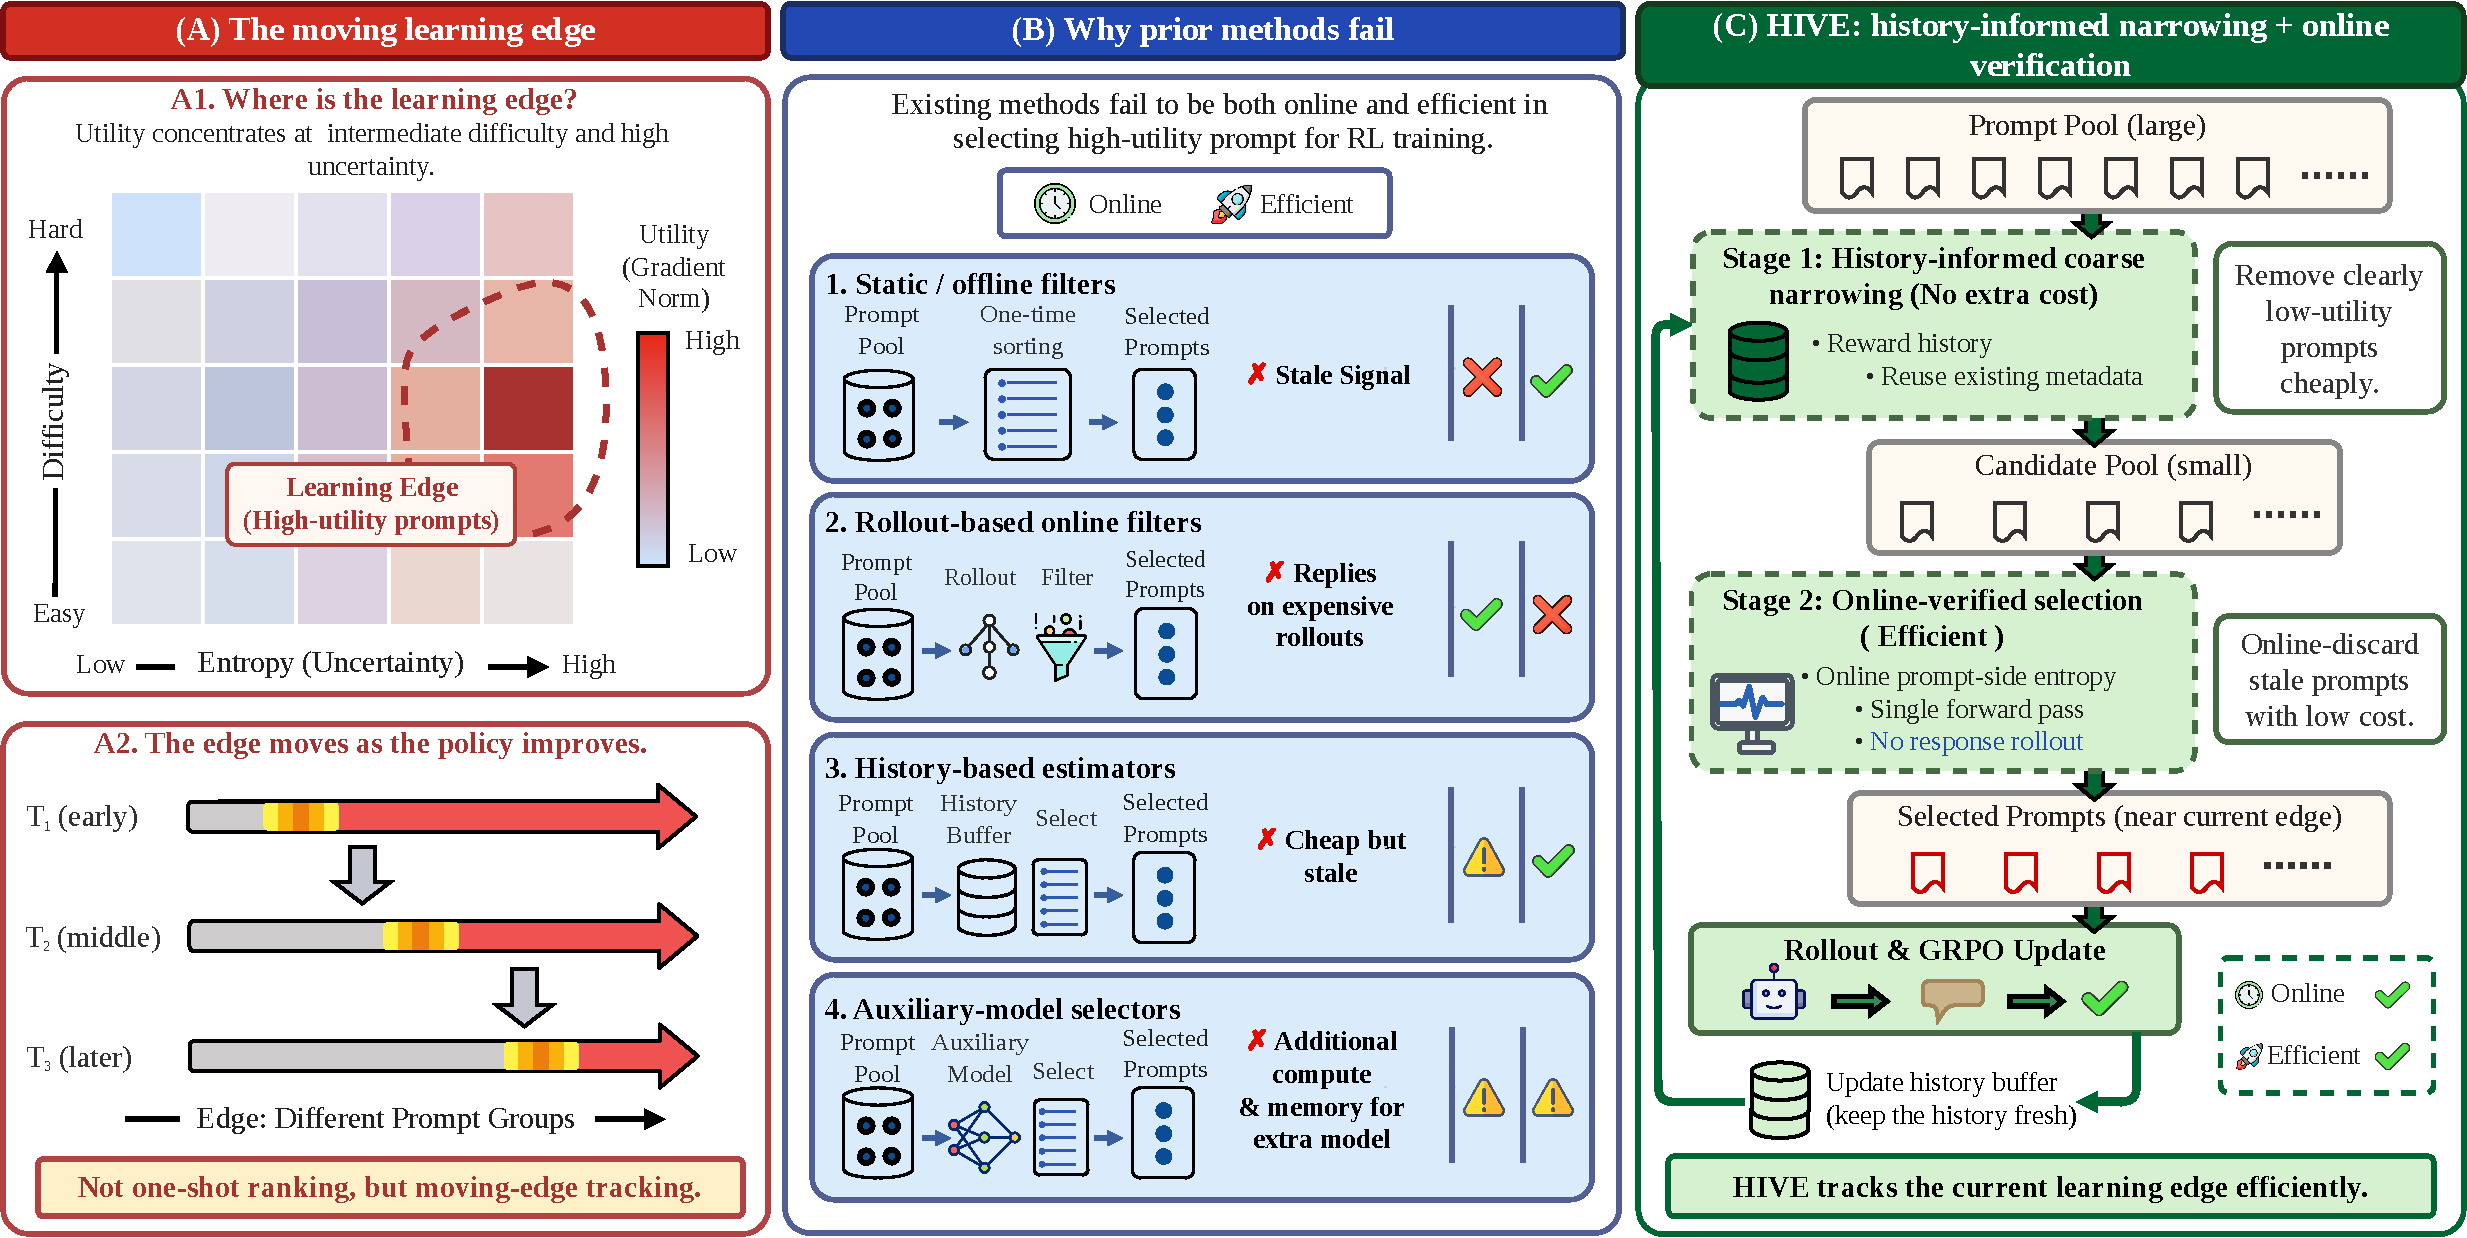
\includegraphics[width=0.98\linewidth]{figures/introduction/intro-fig-compare-motivate-1.pdf}
    \caption{\textbf{RLVR prompt selection is a moving-edge tracking problem.} (A) Utility concentrates at 
    intermediate difficulty and high uncertainty, and the learning edge is dynamic. 
    (B) Prior methods face limitations in efficiently selecting online high-utility prompts. (C) HIVE combines history-informed coarse narrowing with low-cost online 
    verification to track the current learning edge.}
    \label{fig:intro-compare-motivate}
    \vskip -0.2in
\end{figure}
% \red{1. re-write this caption 2.
%     delete precise. 3. redraw figure 3(d) to correspond to the A2 in figure 1. 4. shoud not be like curriculum, 
%     instead the utility of prompts across different step should be varying.}

\section{Introduction}
\label{sec:introduction}
Reinforcement Learning (RL) has emerged as a prevalent paradigm for fine-tuning large language models (LLMs), particularly for enhancing complex mathematical and logical reasoning capabilities~\cite{guo2025deepseek,yu2025dapo,tomihari2026learningdynamicsrlposttraining}. While advanced RL algorithms such as group relative policy optimization (GRPO)~\cite{shao2024deepseekmath} rely on rollout scaling to stabilize training and enhance model performance, they introduce a severe computational overhead~\cite{xu2025not,yu2025dapo,li2026stalefeedbackcoevolvingcritics}. In the training of those RL algorithms, a large portion of computational resources is wasted on generating rollouts for low-utility prompts that are either too trivial or too intractable for the current model. This results in vanishing gradients and wasted resources, providing no informative learning signal for model updates~\cite{zheng2025act,yu2025dapo,noukhovitch2025fasterICLR,verl2025}. Therefore, we investigate the following research question in this paper: \textit{how to identify prompts that are likely to produce useful gradients before rollout?}

Existing methods face limitations in efficiently selecting {high-utility} prompts in an online manner. Static or offline filters rank prompts before training using fixed heuristics, making them inexpensive but unable to adapt to the changing model during RL 
training~\cite{Wang2025ReinforcementLF,Li2025LIMRLI,ye2025limo}. Rollout-based online filters, such as dynamic sampling, better capture the current utility of each prompt by checking reward variance from newly generated responses~\cite{yu2025dapo,xu2025not,Chen2025LSPO,Ye2025PROF}. However, they already incur substantial rollout cost. History-based estimators such as GRESO~\cite{zheng2025act} avoid additional 
rollout cost by estimating prompt utility from past reward statistics, but those metadata becomes stale as the policy 
updates~\cite{zheng2025act,sun2025dots,li2026stalefeedbackcoevolvingcritics}. Auxiliary-model selectors, such as PCL~\cite{Gao2025PCL}, attach external or jointly trained predictors to estimate prompt difficulty or utility, introducing extra compute and memory during selection. 

% To understand what makes a prompt useful during RL training, we first conduct an empirical analysis of GRPO 
% training dynamics.  
% Among prompts with non-zero gradients, high response-side entropy prompts yield stronger learning progress at the same 
% rollout budget (Figure~\ref{fig:intro-a-b}b). More broadly, utility (\red{which we measured via length-normalized gradient norm}) concentrates at the intersection 
% of \red{intermediate difficulty} and high response-side entropy (Figure~\ref{fig:intro-a-b}c), which we term as 
% {learning edge}. However, the edge moves: prompts selected by those historical metadata quickly 
% lose real-time utility, whereas prompts verified under the current policy retain higher gradient norms 
% (Figure~\ref{fig:intro-a-b}a,\ref{fig:intro-a-b}d). Based on these observations, we conclude that an ideal prompt selection 
% framework for efficient LLM RL must be: \textbf{online} to track the moving learning edge, and \textbf{efficient} to avoid excessive overhead for selection.
% To identify what makes a prompt useful during RL training, we first empirically analyze GRPO training dynamics. Among prompts with non-zero gradients, those with high response-side entropy produce greater learning progress under the same rollout budget (Figure~\ref{fig:intro-a-b}b). More broadly, utility, measured by the length-normalized gradient norm, concentrates at the intersection of intermediate difficulty and high response-side entropy (Figure~\ref{fig:intro-a-b}c), which we refer to as the learning edge. However, this edge is dynamic: prompts selected using historical metadata quickly lose real-time utility, whereas prompts verified under the current policy retain higher gradient norms (Figure~\ref{fig:intro-a-b}a,\ref{fig:intro-a-b}d). These observations suggest that an effective prompt selection framework for efficient LLM RL should be \textbf{online}, to track the moving learning edge, and \textbf{efficient}, to avoid excessive selection overhead.
To identify what makes a prompt useful during RL training, we first empirically analyze GRPO training dynamics. Among prompts with non-zero gradients, those with high response-side entropy produce greater learning progress under the same rollout budget (Figure~\ref{fig:intro-high-entropy}). More broadly, utility, measured by the length-normalized gradient norm, concentrates at the intersection of intermediate difficulty and high response-side entropy (Figure~\ref{fig:intro-learning-edge}), which we refer to as the learning edge. However, this edge is dynamic: prompts selected using historical metadata quickly lose real-time utility, whereas prompts verified under the current policy retain higher gradient norms (Figures~\ref{fig:intro-history-staleness}); prompts move substantially among High, Low, and Zero utility classes across training steps (Figure~\ref{fig:intro-utility-shift}). These observations suggest that an effective prompt selection framework for efficient LLM RL should be \textbf{online}, to track the moving learning edge, and \textbf{efficient}, to avoid excessive selection overhead.
% To identify what makes a prompt useful during RL training, we first empirically analyze GRPO training dynamics. Among prompts with non-zero gradients, those with high response-side entropy produce greater learning progress under the same rollout budget (Figure~\ref{fig:intro-high-entropy}). More broadly, utility, measured by the length-normalized gradient norm, concentrates at the intersection of intermediate difficulty and high response-side entropy (Figure~\ref{fig:intro-learning-edge}), which we refer to as the learning edge. However, this edge is dynamic: prompts selected using historical metadata quickly lose real-time utility, whereas prompts verified under the current policy retain higher gradient norms (Figure~\ref{fig:intro-history-staleness}); prompts also move substantially among High, Low, and Zero utility classes across training steps (Figure~\ref{fig:intro-utility-shift}). These observations suggest that an effective prompt selection framework for efficient LLM RL should be \textbf{online}, to track the moving learning edge, and \textbf{efficient}, to avoid excessive selection overhead.


% To understand what makes a prompt useful for RL training, we first empirically examine GRPO training dynamics. Among prompts with non-zero gradients, those with higher response-side entropy yield greater learning progress under the same rollout budget (Figure~\ref{fig:intro-high-entropy}). More generally, utility, measured by the length-normalized gradient norm, is concentrated where intermediate difficulty and high response-side entropy intersect (Figure~\ref{fig:intro-learning-edge}); we refer to this region as the \emph{learning edge}. However, this edge shifts over time: prompts selected using historical metadata rapidly lose real-time utility, whereas prompts verified under the current policy maintain higher gradient norms (Figure~\ref{fig:intro-history-staleness}). Moreover, prompts frequently transition among High-, Low-, and Zero-utility classes throughout training (Figure~\ref{fig:intro-utility-shift}). These findings suggest that an effective prompt selection framework for efficient LLM RL should be both \textbf{online}, to track the moving learning edge, and \textbf{efficient}, to minimize selection overhead.

Based on previous analysis, we propose \textbf{HIVE} (\textbf{H}istory-\textbf{I}nformed \textbf{V}erification of the learning \textbf{E}dge), a dual-stage 
framework for rollout-efficient RLVR (Figure~\ref{fig:framework}). HIVE first performs history-informed coarse narrowing using 
reward trajectories and response-side entropies accumulated from previous training steps. This stage targets efficiency by retaining exploration probability for prompts that are around the edge. HIVE then utilizes prompt entropy as a high-fidelity and efficient proxy to perform online verification under the current policy, filtering stale candidates before the rollout phase.
% HIVE then performs online verification with prompt-side entropy 
% computed under the current policy. This stage restores online precision and filters 
% stale candidates before the rollout phase.

% Evaluation for HIVE is conducted across multiple reasoning benchmarks (e.g., {math, coding, and tool calling}) and models: Qwen3-4B~\cite{yang2025qwen3technicalreport}, 
Evaluation for HIVE is conducted across multiple reasoning benchmarks (e.g., math and tool calling) and models: Qwen3-4B-Base~\cite{yang2025qwen3technicalreport}, 
Qwen2.5-Math-1.5B/7B~\cite{yang2024qwen25mathtechnicalreportmathematical}, DeepSeek-R1-Distill-Qwen-1.5B~\cite{guo2025deepseek}, 
% Qwen2.5-14B/32B~\cite{qwen2.5-large}, and Llama-3.2-3B-Instruct~\cite{grattafiori2024llama3}. HIVE maintains comparable or better accuracy than Dynamic Sampling~\cite{yu2025dapo}, Pre-filter, GRESO~\cite{zheng2025act}, and PCL~\cite{Gao2025PCL} while using fewer rollouts, achieving up to \textbf{3.8$\times$ speedup in rollout} and \textbf{2.3$\times$ faster total training time} for models like Qwen2.5-Math-7B. Finally, we show that HIVE drastically lowers computational overhead, reducing rollouts by \textbf{up to 9.2 million} while consistently maintaining or even exceeding the reasoning accuracy of strong selection baselines across DAPO+MATH, Open-R1, and larger Qwen2.5 model scales.
Qwen2.5-14B/32B~\cite{qwen2.5-large}, and Llama-3.2-3B-Instruct~\cite{grattafiori2024llama3}. HIVE significantly outperforms 
baselines like Dynamic Sampling~\cite{yu2025dapo}, GRESO~\cite{zheng2025act} and PCL~\cite{Gao2025PCL}, achieving up to \textbf{2.3$\times$ faster total training time} for models like Qwen2.5-Math-7B. Finally, we show that HIVE lowers computational 
overhead, achieving \textbf{up to 9.2 million rollouts reduction} while consistently maintaining the reasoning performance. Beyond mathematical reasoning, HIVE also attains the best BFCL-V2 tool-calling score while using \textbf{4.8$\times$ fewer rollouts} than Dynamic Sampling, suggesting that moving-edge tracking extends to verifiable tool-use tasks.
%Besides, \red{the studies on coding and tool-calling tasks also show the generality of HIVE beyond math reasoning.}
% Our contributions are threefold:
% \begin{itemize}[topsep=2pt,itemsep=1pt,leftmargin=*]
%     and efficient required for practical selection. 
%     \item We propose HIVE, a dual-stage selector that combines zero-cost history-informed narrowing with low-cost online verification. 
%     \item We demonstrate across multiple tasks and model scales that HIVE significantly reduces rollout and wall-clock training costs while 
%     preserving or improving performance on those tasks.
% \end{itemize}
% Table 2 (Open-R1) and Figure 5 (Qwen2.5-14B/32B) merged into a single
% top-of-page side-by-side float for compactness.
% \documentclass{article}
% \usepackage{booktabs}
% \usepackage{graphicx}
% \usepackage{caption} % 必须引入，用于支持 \captionof

% \begin{document}

\begin{table*}[t]
    \centering
    % ==========================
    % 左侧：表格 (占约 64% 宽度)
    % ==========================
    % \hfill % 中间弹性间距
    % ==========================
    % 右侧：图片 (占约 32% 宽度)
    % ==========================
    \begin{minipage}[c]{0.255\textwidth}
        \centering
        % 插入图片
        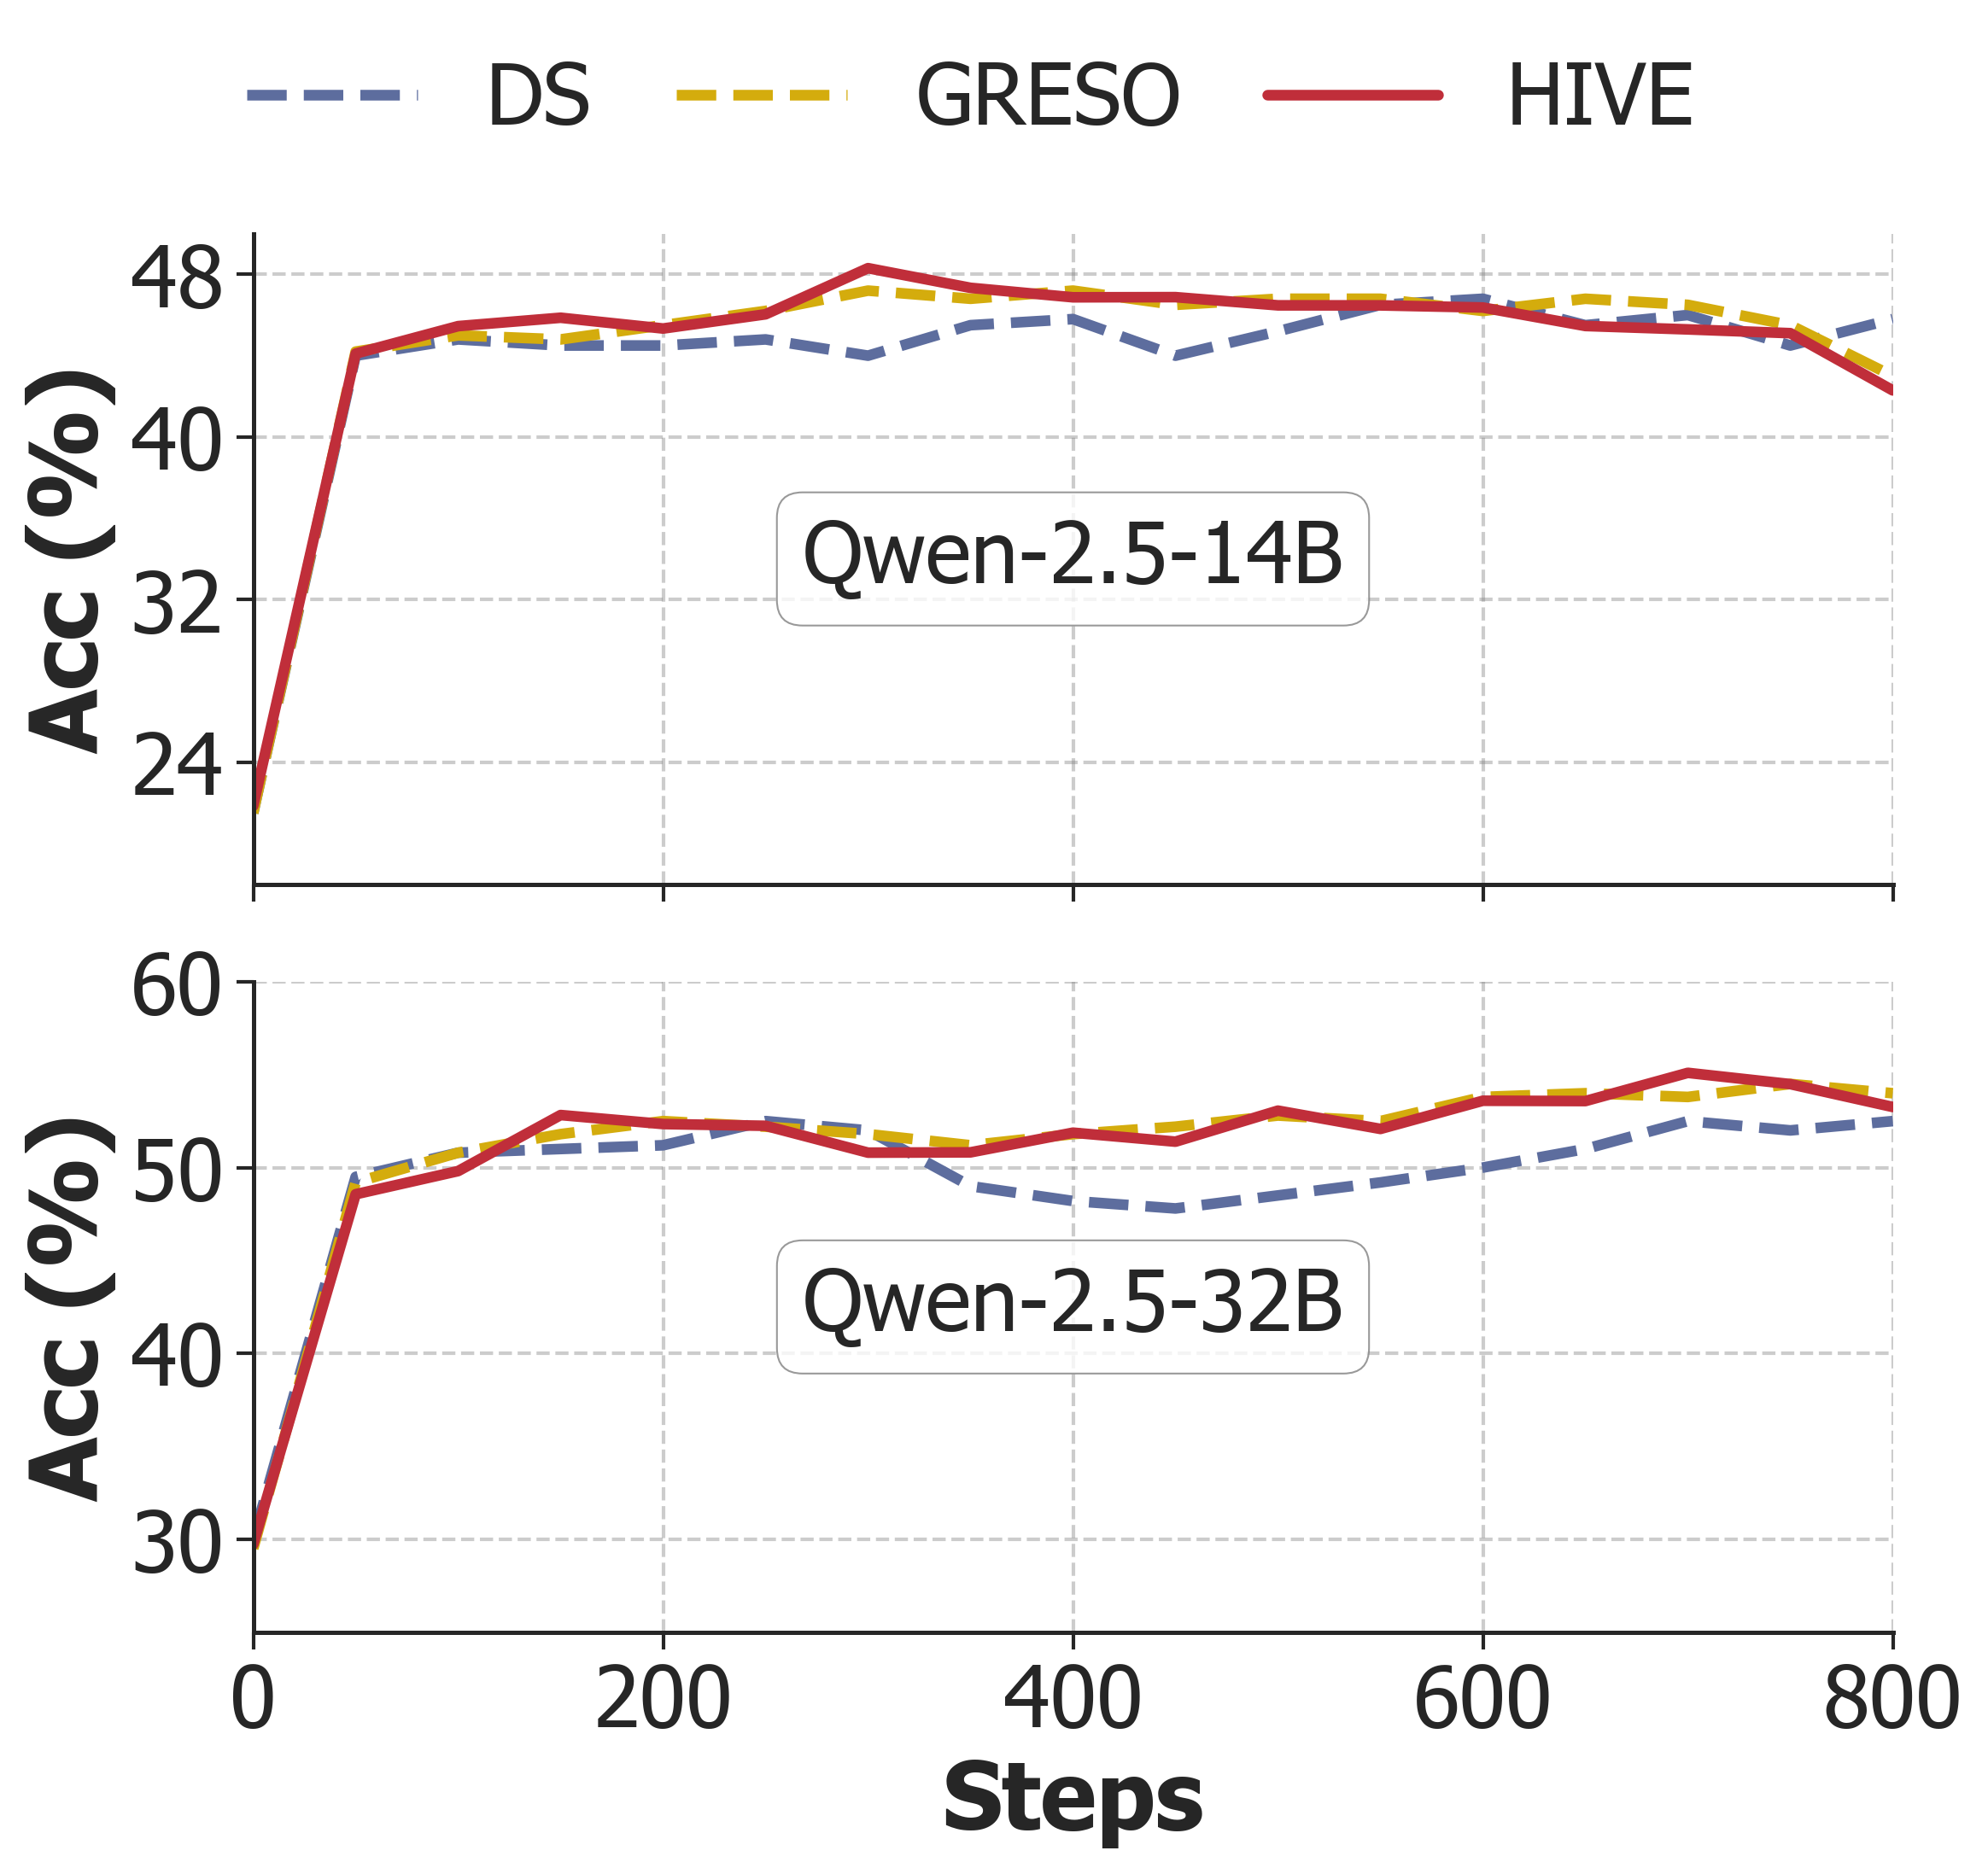
\includegraphics[width=\linewidth]{figures/experiment/12-scale-to-14b-32b_styled_vertical.png}
        % 使用 captionof{figure} 给图片正确编号
        \captionof{figure}{Scaling up to Qwen2.5-14B/32B.}
        \label{fig:scale_14b_32b}
    \end{minipage}
    \hfill
        \begin{minipage}[c]{0.735\textwidth}
        \centering
        \caption{Performance (\%) and rollout comparison of Qwen2.5-Math-1.5B and Qwen2.5-Math-7B trained on Open-R1.}
        \label{tab:openr1-main-exp}
        
        % 使用 resizebox 确保宽表格能完美放入左侧空间
        \resizebox{\linewidth}{!}{
            \begin{tabular}{c|cccccc|c|c}
            \toprule
            {Method} & {Math500} & {AIME24} & {AMC} & {Gaokao} & {Miner.} & {Olymp.} & {Avg.} & {\#Rollout} \\
            \midrule
            
            % Block 1: Qwen2.5-Math-1.5B
            \multicolumn{9}{c}{{\textit{Qwen2.5-Math-1.5B}}} \\
            \midrule
            DS    & 77.1 & 16.7 & 50.3 & 65.5 & 30.9 & 39.7 & 46.7 & 3.8M (1.0$\times$) \\
            GRESO & 76.1 & 20.0 & 50.6 & 65.1 & 30.0 & 39.2 & 46.8 & 1.6M (2.4$\times$)\\
            HIVE  & 76.9 & 18.3 & 48.7 & 65.4 & 30.1 & 40.3 & 46.6 & \best{{1.5M} (2.5$\times$)} \\
            \midrule
            
            % Block 2: Qwen2.5-Math-7B
            \multicolumn{9}{c}{{\textit{Qwen2.5-Math-7B}}} \\
            \midrule
            DS    & 82.8 & 34.2 & 63.5 & 67.3 & 35.7 & 46.3 & 55.0 & 11.4M (1.0$\times$) \\
            GRESO & 82.3 & 35.0 & 64.4 & 66.8 & 36.5 & 45.7 & 55.1 & 3.4M (3.4$\times$) \\
            HIVE  & 82.6 & 36.7 & 63.9 & 66.7 & 36.2 & 45.9 & 55.3 & \best{2.5M (4.7$\times$)} \\
            \bottomrule
            \end{tabular}
        }
    \end{minipage}
    \vskip -0.2in
\end{table*}
% \end{document}


\best{HIVE preserves accuracy while reducing rollouts.}
We compare HIVE against Dynamic Sampling (DS)~\cite{yu2025dapo}, a rollout-based online filter, and GRESO~\cite{zheng2025act}, a history-based selector. Table~\ref{tab:model_performance} reports results on DAPO+MATH across four model families. HIVE consistently uses fewer rollouts than both baselines while maintaining comparable average accuracy. On Qwen2.5-Math-7B, HIVE reduces rollouts by 70\% compared with DS (13.1M to 3.9M) and achieves the highest average accuracy (59.7\% vs. 57.8\% for DS and 58.6\% for GRESO), reaching comparable accuracy with substantially fewer generated responses.

\best{The gains transfer across datasets and model scales.}
Table~\ref{tab:openr1-main-exp} evaluates Qwen2.5-Math-1.5B/7B on Open-R1. HIVE again keeps comparable or better average accuracy while reducing rollouts, reaching 4.7$\times$ fewer rollouts than DS on Qwen2.5-Math-7B. Figure~\ref{fig:scale_14b_32b} extends the comparison to Qwen2.5-14B and Qwen2.5-32B. HIVE follows a similar convergence trajectory to DS and GRESO while requiring fewer rollouts; for Qwen2.5-14B over 800 steps, HIVE uses 1.56M rollouts compared with 1.74M for GRESO and 3.45M for DS.

\best{Wall-clock savings come from rollout reduction, not hidden overhead.}
Table~\ref{tab:efficiency_cost} decomposes end-to-end training time. HIVE reduces rollout time by up to 3.8$\times$ and total training time by up to 23$\times$ over DS. On Qwen2.5-Math-7B, total training time drops from 198.4 hours (DS) and 112.3 hours (GRESO) to 85.8 hours (HIVE), while rollout time drops from 153.7 and 66.3 to 40.2.

\begin{wraptable}[10]{r}{0.4\textwidth}
    \vspace{-1.2em}
    % \vskip -0.2in
    \centering
    \caption{Performance comparison (\%) on tool calling tasks.}
    \label{tab:tool_calling}
    \small
    \setlength{\tabcolsep}{3.2pt}
    \renewcommand{\arraystretch}{0.92}
    \begin{tabular}{lcc}
        \toprule
        Method & BFCL-V2 & \#Rollout \\
        \midrule
        DS & 79.08 & 5.3M \\
        Pre-filter & 77.04 & 1.4M \\
        GRESO & 78.96 & 1.4M \\
        PCL & 76.84 & 1.4M \\
        HIVE & \best{79.26} & \best{1.1M} \\
        \bottomrule
    \end{tabular}
    \vspace{-1.2em}
    % \vskip -0.2in
\end{wraptable}
\noindent\best{Performance on tool calling tasks.} Besides, we also verify the effectiveness of HIVE on tool calling tasks. We train Qwen2.5-1.5B on 80\% prompts samples from BFCL-V2~\cite{gorilla-openfunctions-v2} and evaluate the performance on the remaining 20\% subset~\cite{guo2025sample}. As shown in Table~\ref{tab:tool_calling}, HIVE achieves the highest BFCL-V2 score, slightly exceeding DS (79.26 vs. 79.08) while using only 1.1M rollouts instead of 5.3M. This corresponds to a 4.8$\times$ rollout reduction relative to DS. Under the same low-rollout regime, HIVE also outperforms the static Pre-filter baseline, the history-only GRESO selector, and the auxiliary PCL selector. These results suggest that moving-edge tracking is not only specific to mathematical reward signals, but also applicable on tool-calling tasks, where HIVE continues to concentrate rollout compute on informative prompt.

\subsection{Mechanism Analysis: Efficiency and Moving-Edge Adaptation}
\label{subsec:further-experiment}
\begin{figure*}[t]
    \centering
        % 第四张图：Zero-Variance Ratio
    \begin{subfigure}[b]{0.24\textwidth}
        \centering
        % \includegraphics[width=\textwidth]{figures/experiment/9-zero-variance-ratio-comparison-smoothed.png}
        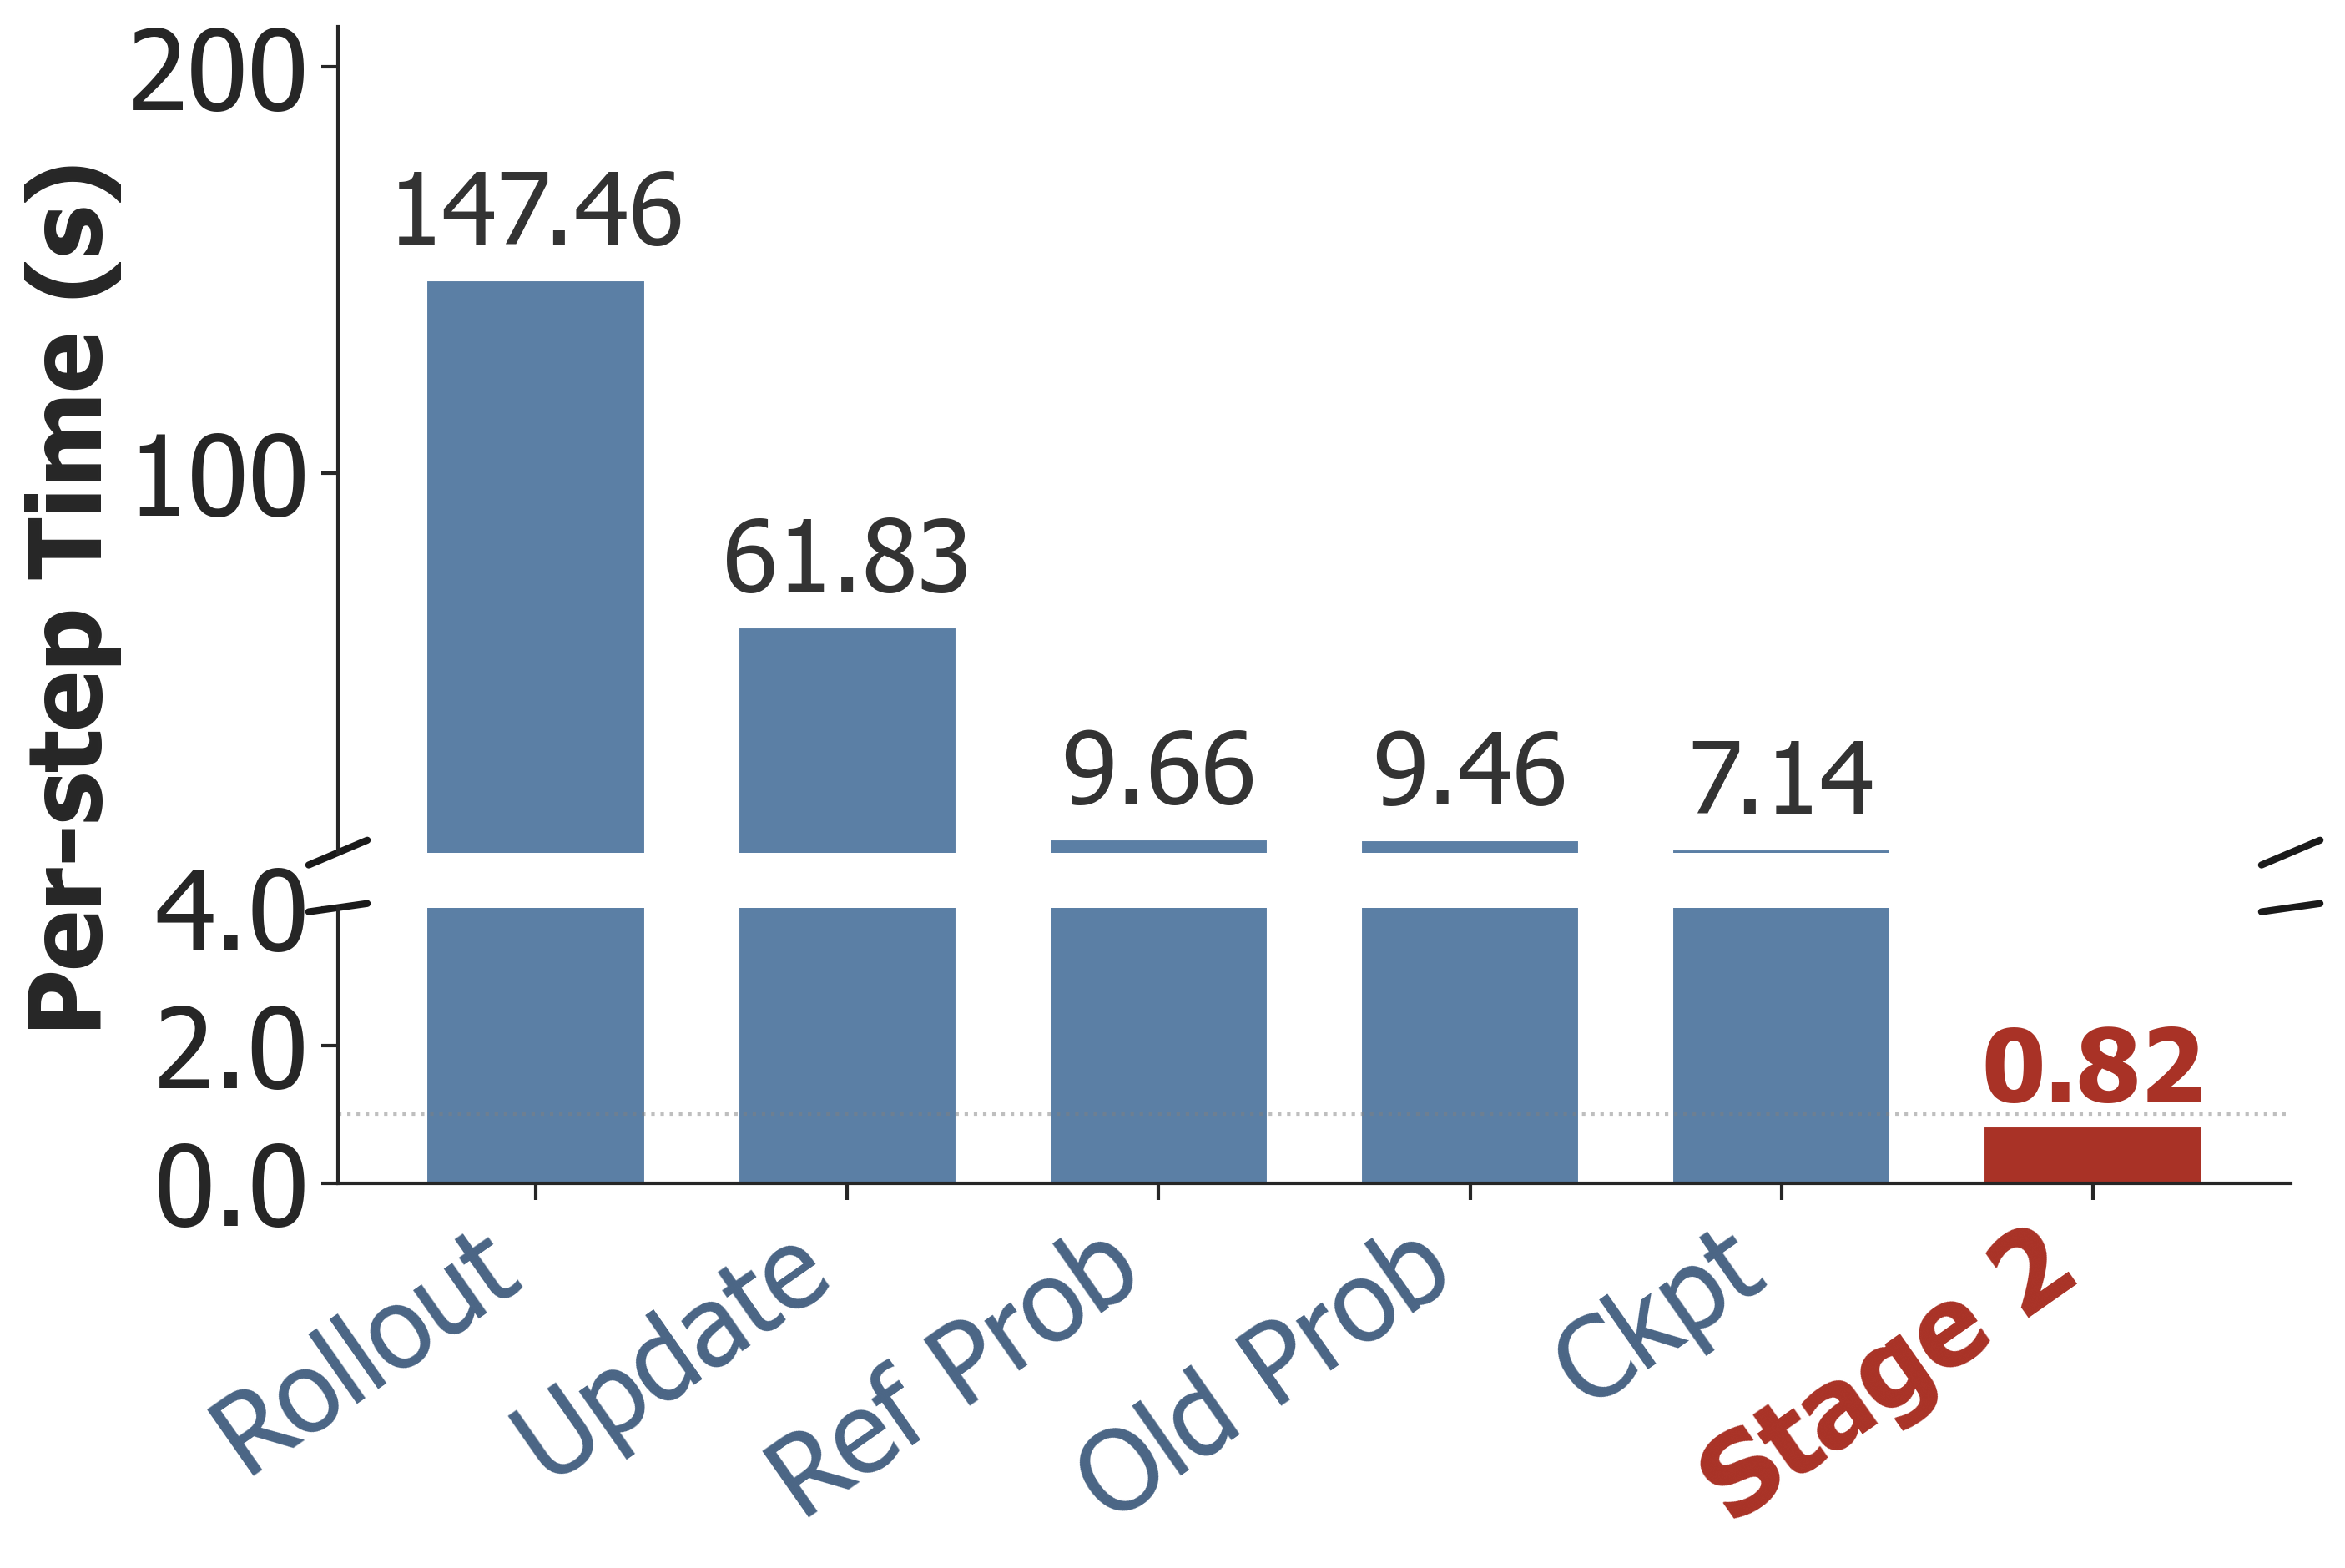
\includegraphics[width=\textwidth]{figures/experiment/5-broken_axis_styled.png}
        \caption{{Train-Time Breakdown}}
        \label{fig:per_step_time_analysis}
    \end{subfigure}
    % 第一张图：Rollout vs Time
    \begin{subfigure}[b]{0.24\textwidth}
        \centering
        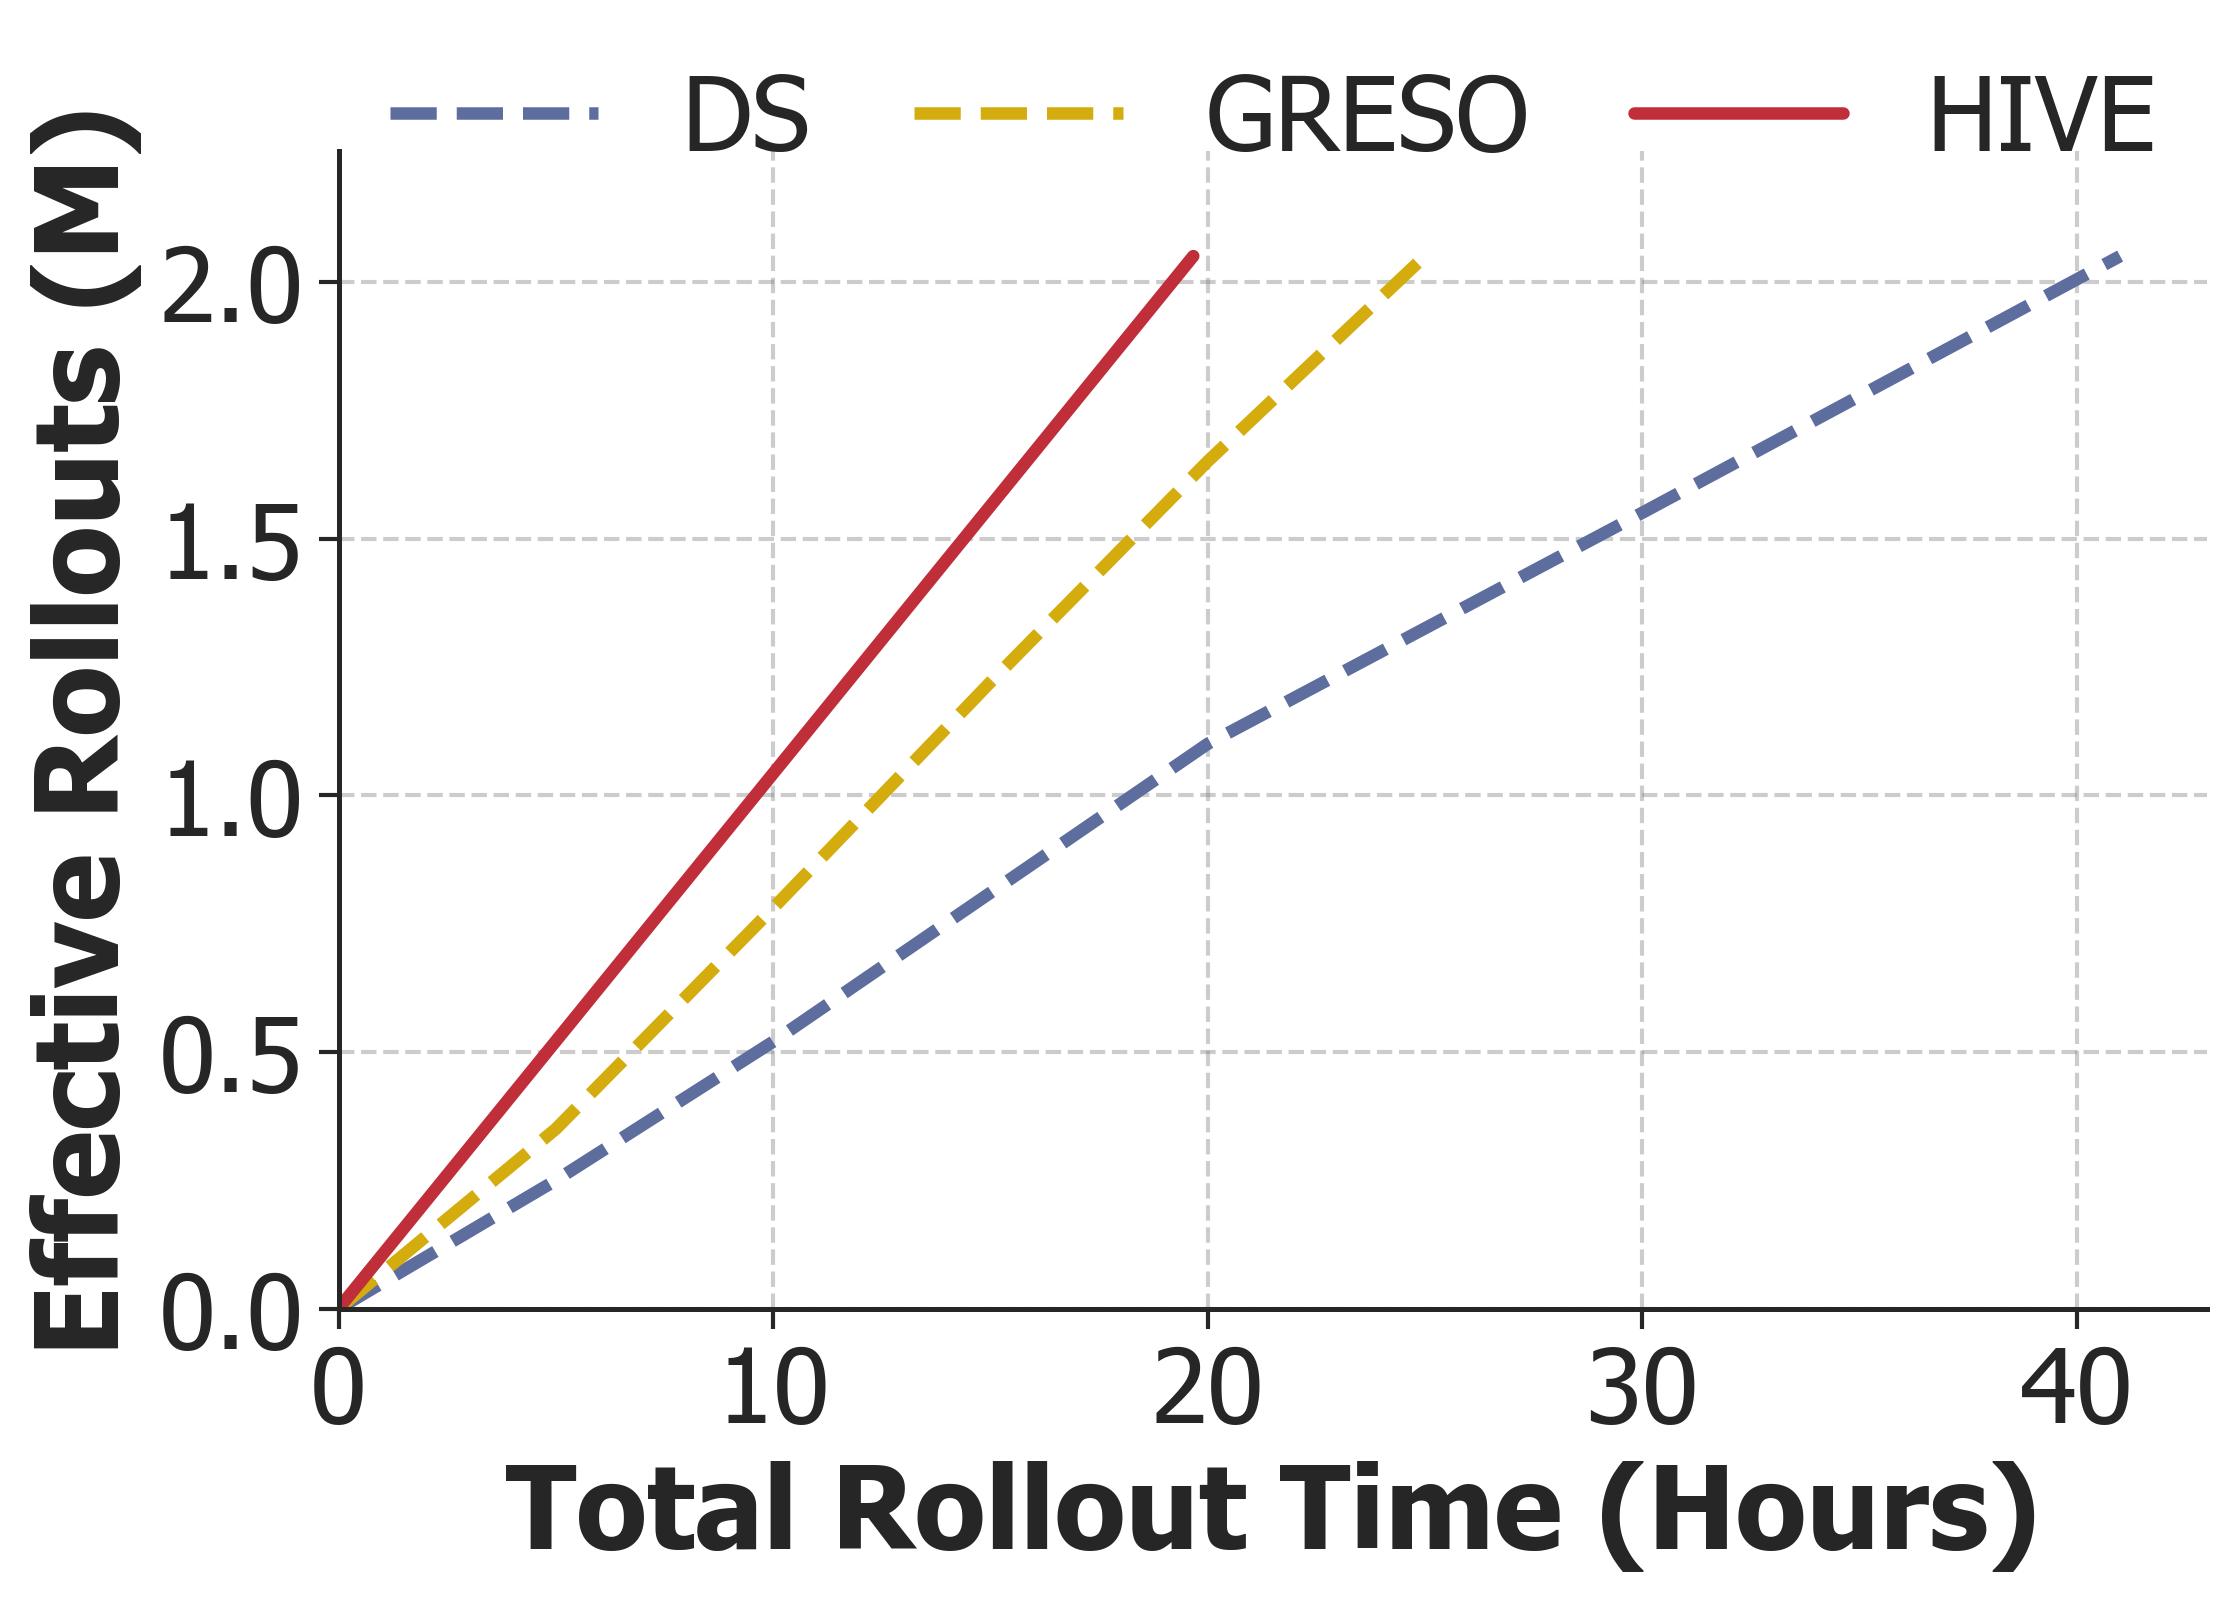
\includegraphics[width=\textwidth]{figures/experiment/11-total-rollout-time-VS-total-effective-rollouts.png}
        \caption{Efficiency Comparison}
        \label{fig:total_rollout}
    \end{subfigure}
    \hfill
    % 第二张图：Generation Time per Step
    \begin{subfigure}[b]{0.24\textwidth}
        \centering
        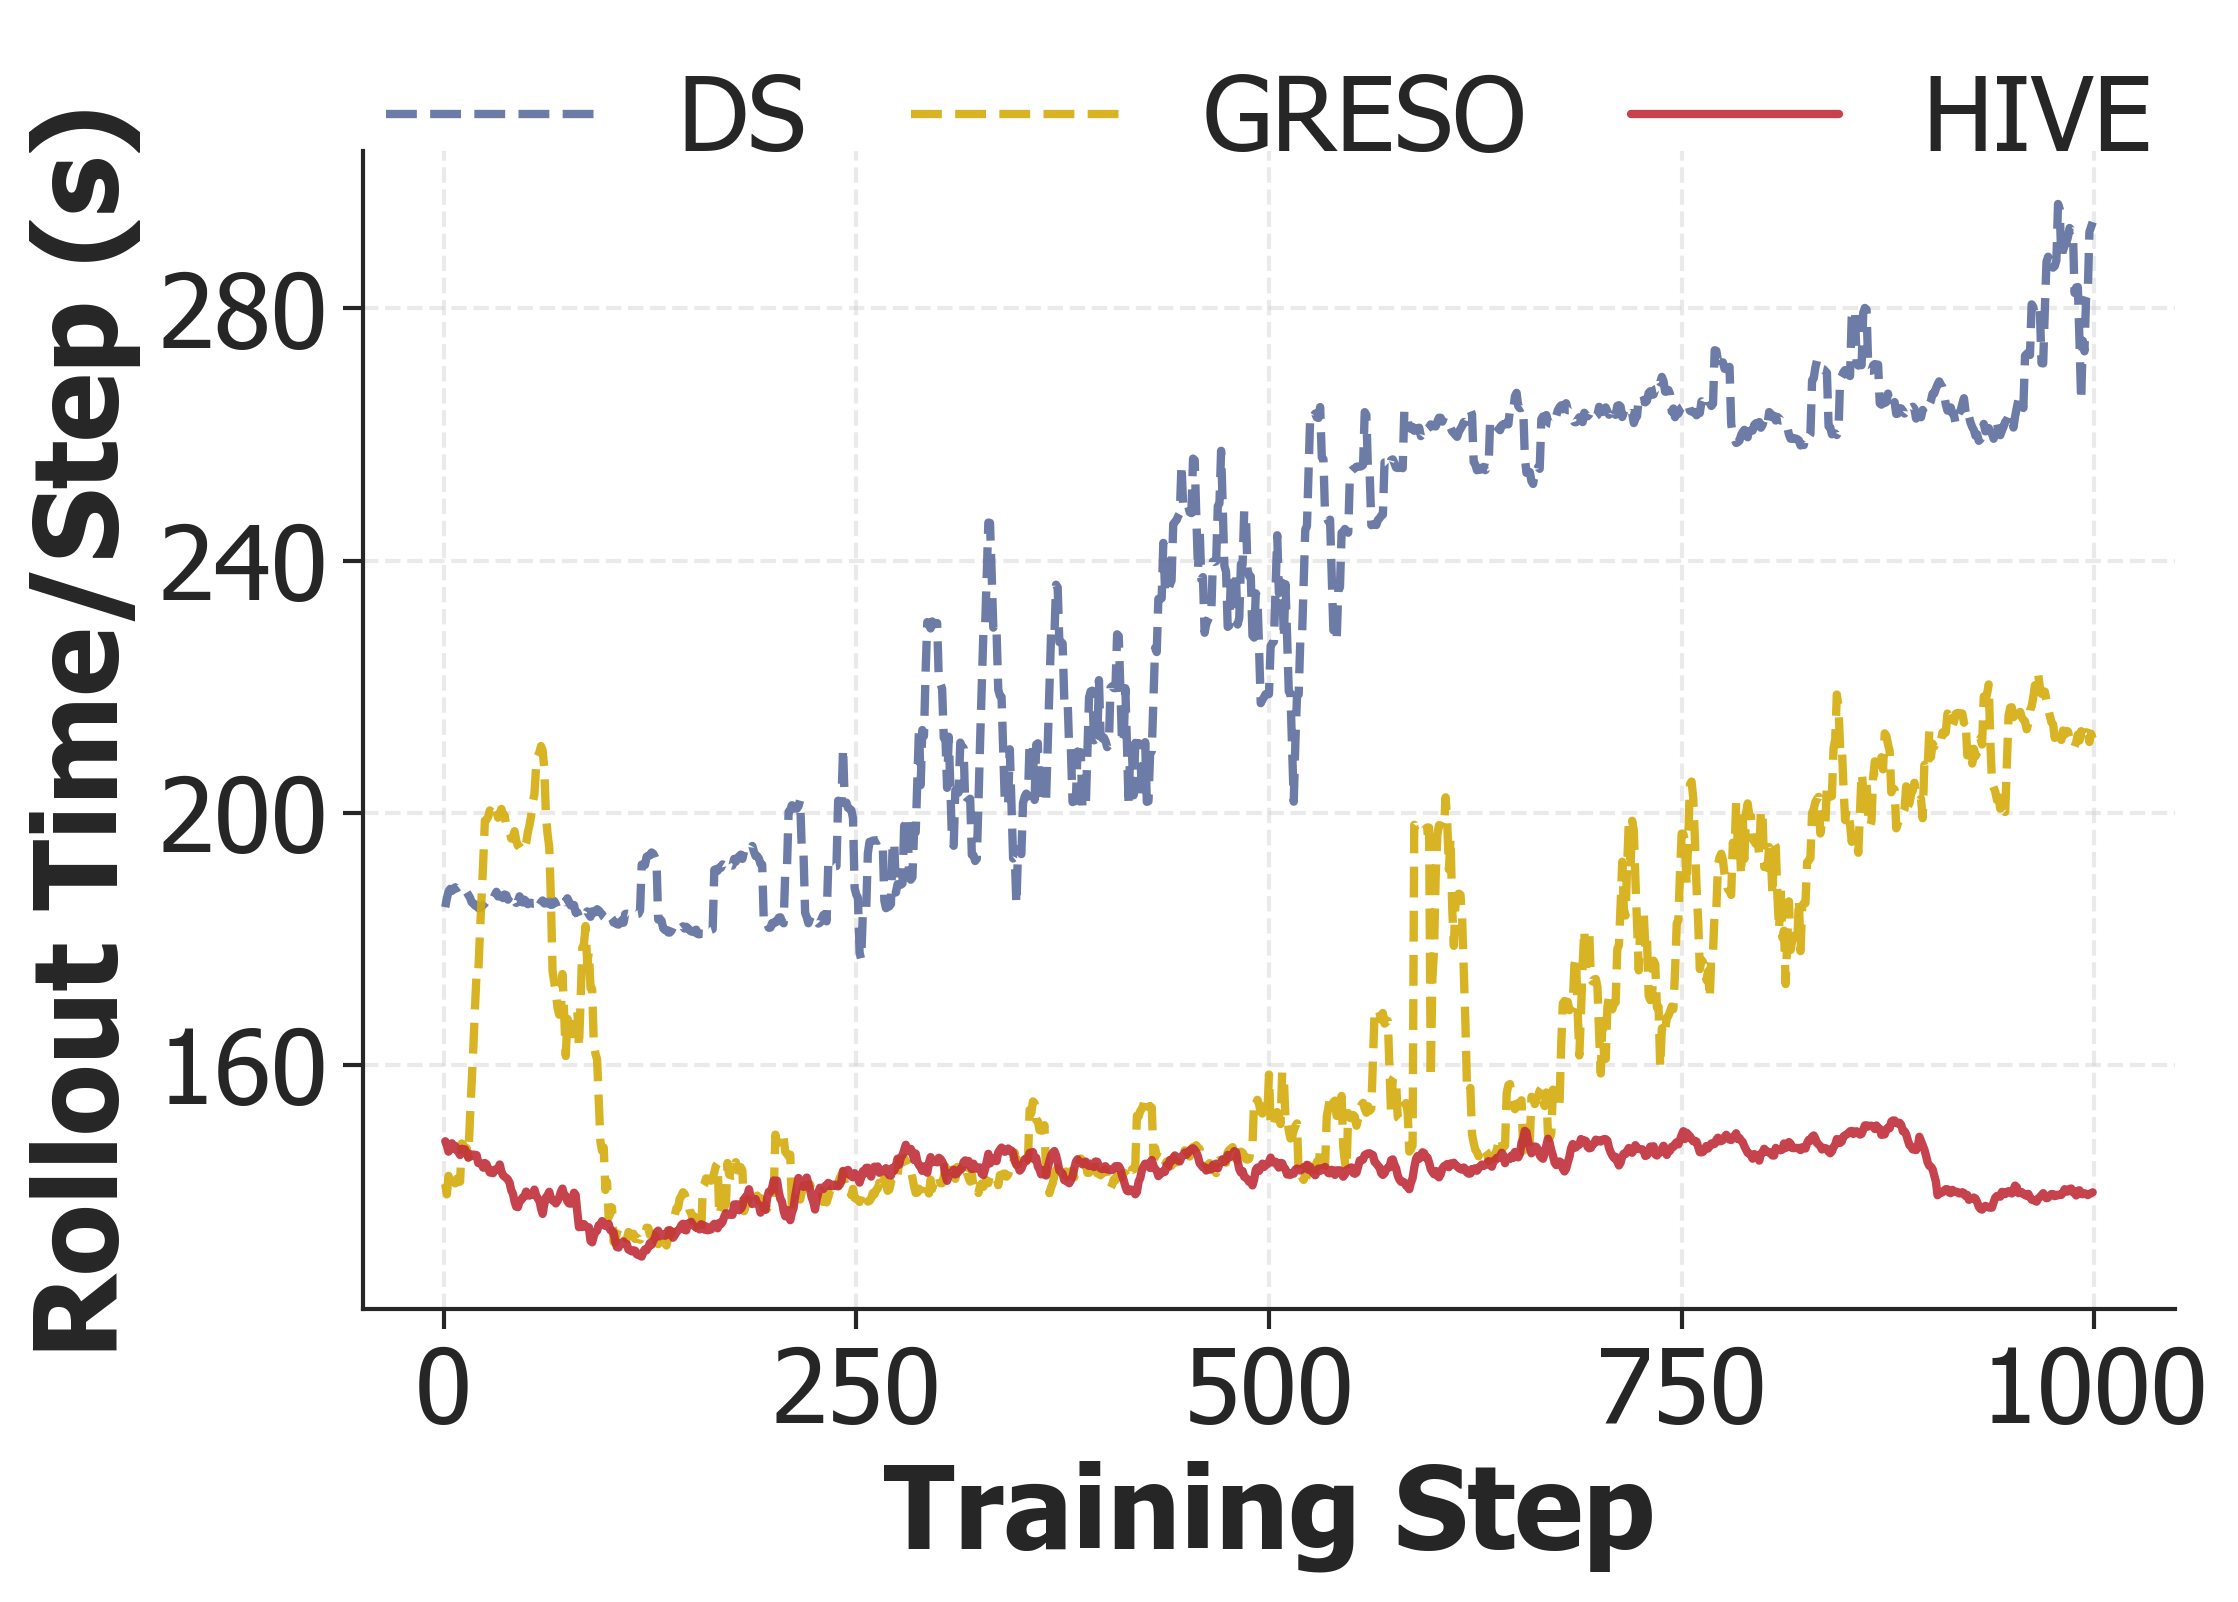
\includegraphics[width=\textwidth]{figures/experiment/10-rollout-time-per-step-comparison-smoothed.png}
        \caption{Generation Time}
        \label{fig:gen_time}
    \end{subfigure}
    \hfill
    % 第三张图：Rollouts per Step
    \begin{subfigure}[b]{0.24\textwidth}
        \centering
        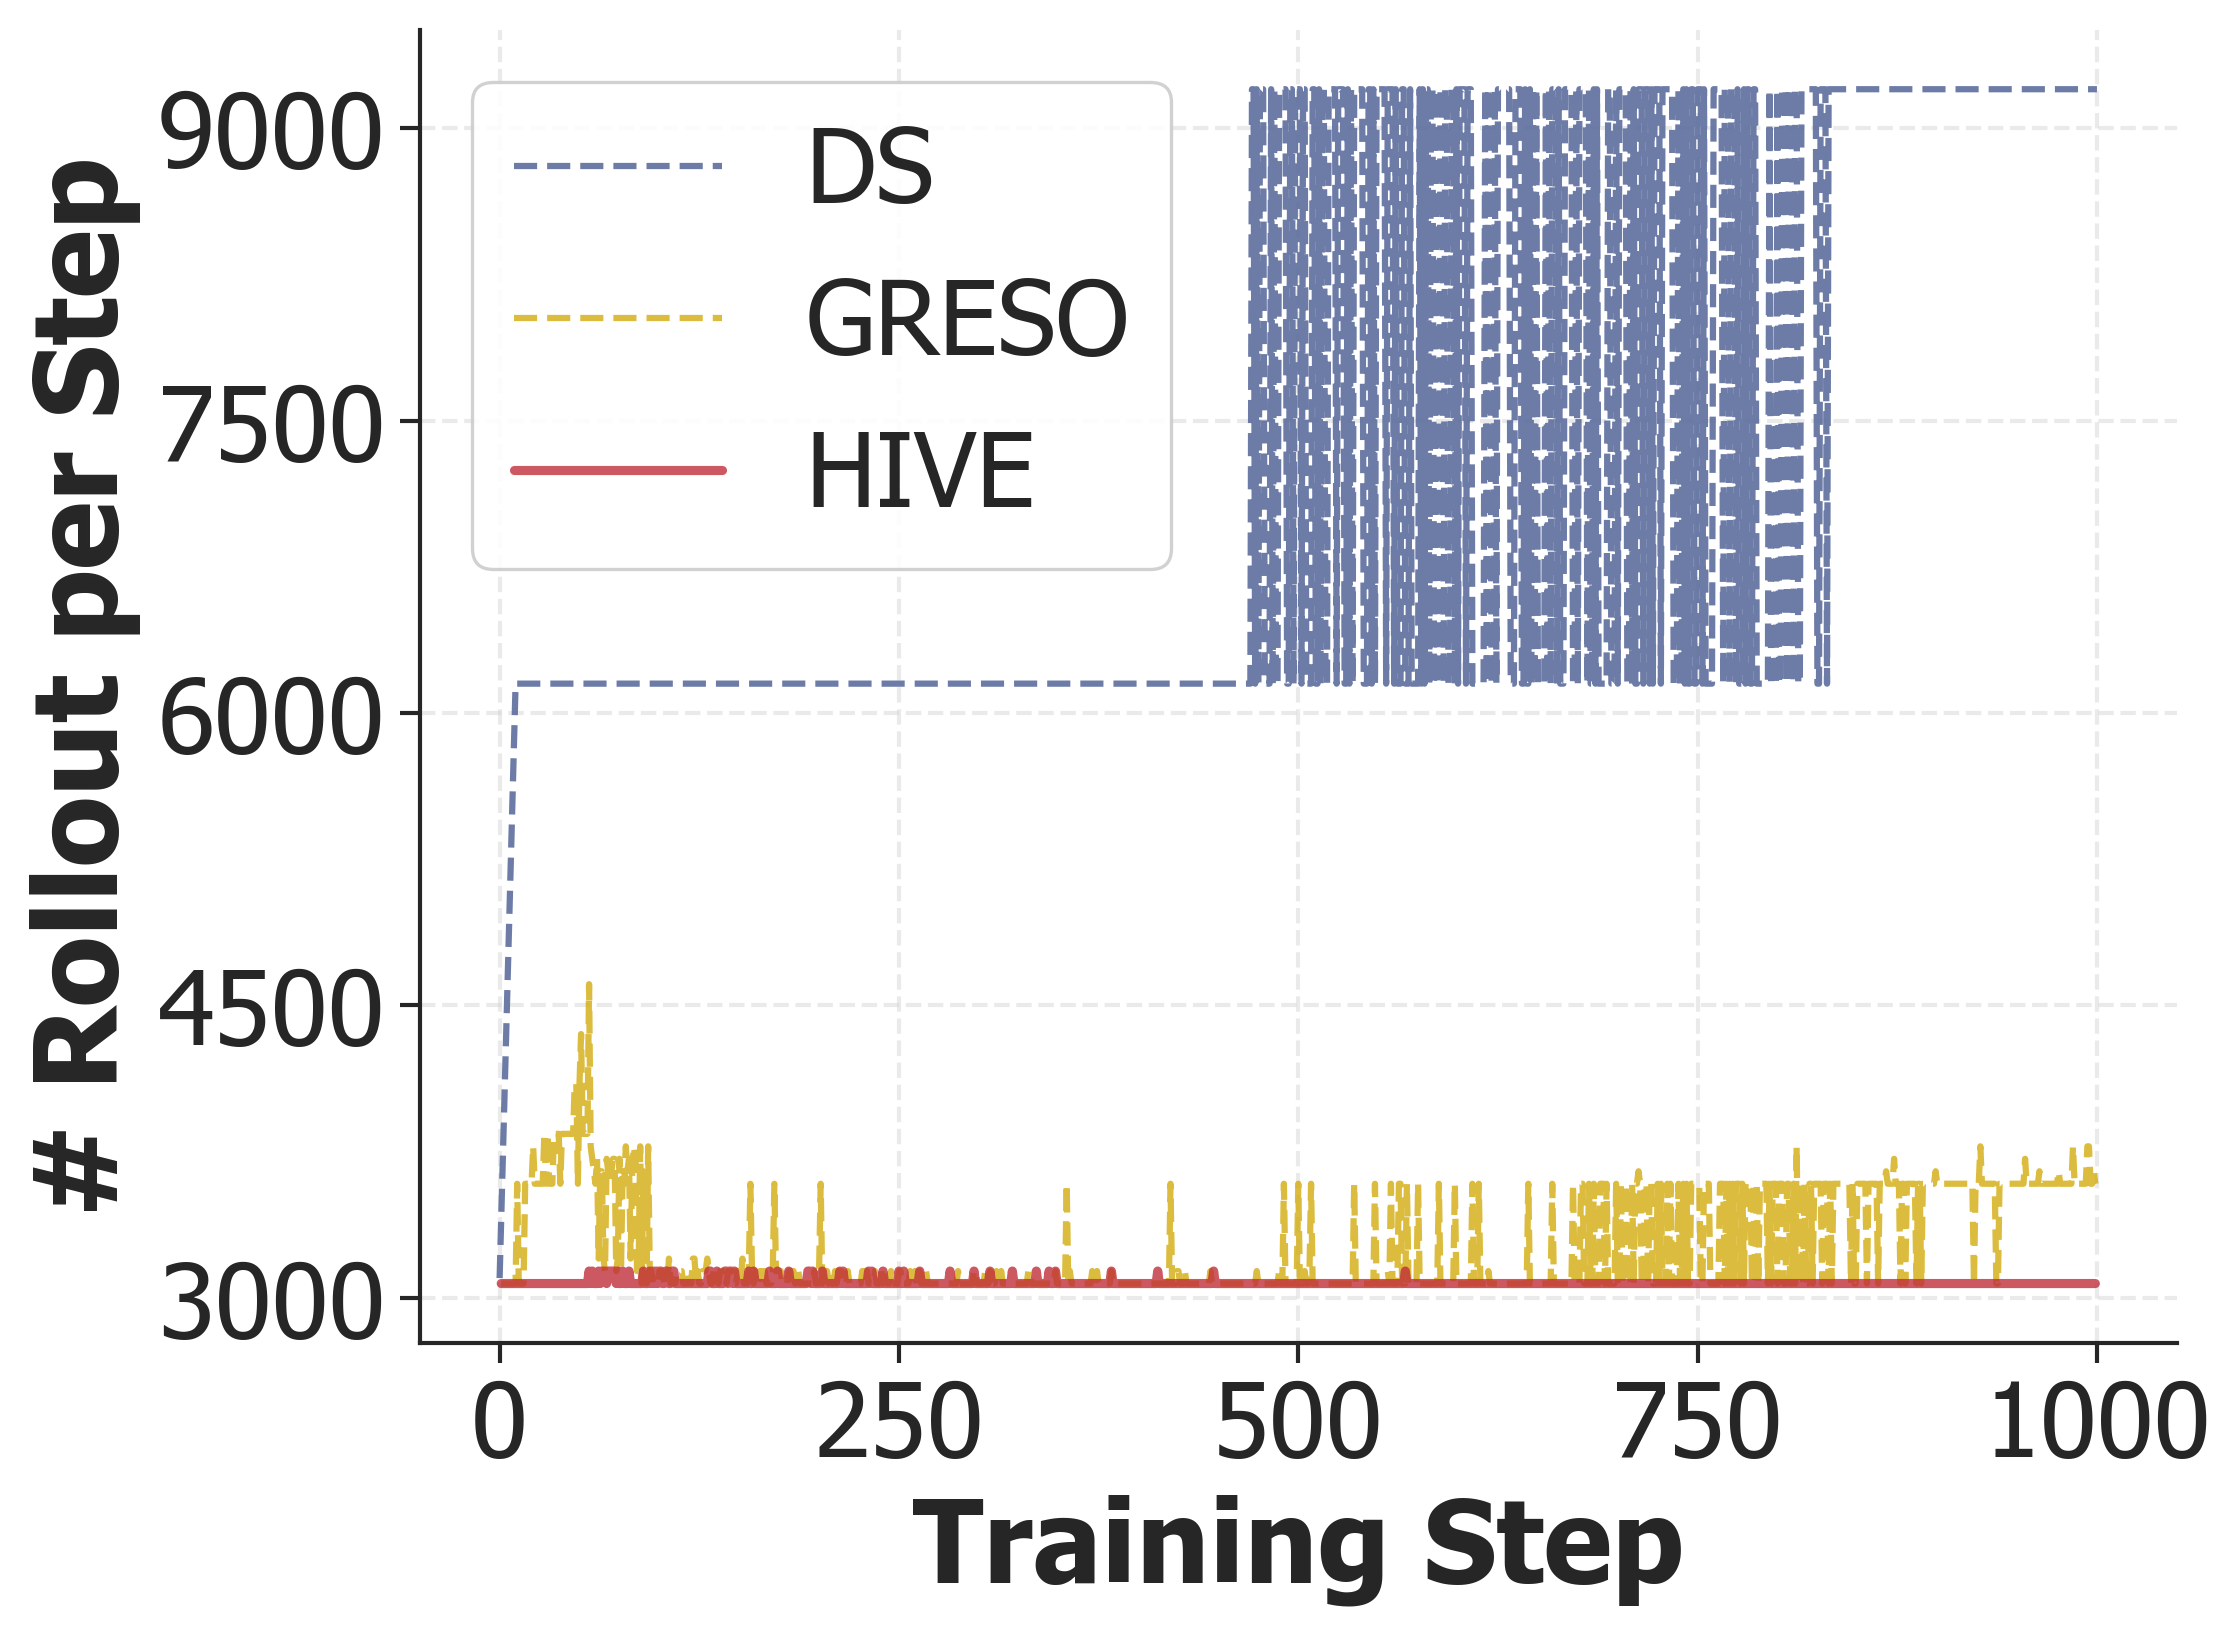
\includegraphics[width=\textwidth]{figures/experiment/8-per-step-rollout-comparison.png}
        \caption{Rollouts per Step}
        \label{fig:rollout_step}
    \end{subfigure}
    \hfill
    
    \caption{Efficiency analysis of Qwen2.5-Math-1.5B trained on DAPO+MATH. (a) Stage~2 prompt-side verification adds little time relative to rollout generation. (b) HIVE accumulates effective rollouts fastest per rollout hour. (c) HIVE maintains lower generation latency throughout training. (d) HIVE rolls out fewer prompt groups per step, concentrating compute on verified candidates.}
    \label{fig:further-analysis}
\end{figure*}


\best{Online verification is cheap enough to run before rollouts.}
Figure~\ref{fig:per_step_time_analysis} isolates the per-step overhead of Stage~2. Computing prompt-side entropy adds only 0.82 seconds, less than 0.4\% of the iteration time, while the rollout phase alone takes 147.46 seconds. This supports the efficiency side of the triad: HIVE gains online information without paying for response generation during selection.

\best{HIVE improves effective rollout throughput.}
Figure~\ref{fig:total_rollout} shows that HIVE accumulates effective rollouts per hour fastest. Figure~\ref{fig:gen_time} further shows that HIVE maintains low rollout-generation latency throughout training, while GRESO becomes slower later in training. This is consistent with metadata staleness: a history-only selector increasingly admits prompts that look useful in the log but no longer produce efficient current updates. Figure~\ref{fig:rollout_step} shows that HIVE also generates fewer rollout groups per step, concentrating compute on a smaller set of verified prompts near the current edge.

% Figure 5 is now combined with Table 2 in sections/exp-table-plux-figure.tex
% (\input-ed near the top of subsection "Main Results"); keeping the
% standalone variants here as comments for reference.
% \input{sections/figures/exp-scale-14b-32b}
% \input{sections/figures/exp-scale-14b-32b-vertical.tex}
% % Single-row top-of-page figure that fuses what used to be Figure 6
% % (zero-variance ratios on Easy / Hard) and Figure 7 (threshold entropy +
% % Stage 1/2 ablation) into one wide composite.
% %
% % The composite PDF is rendered by
% %   ICML2026-submission-figure-script-drawio-todo/wandb-figure/merge4_zerovar_component.py
% %
% % Sub-labels are produced via \phantomsubcaption from the `subcaption`
% % package, so existing \ref{fig:non-zero-diveregence-comparison},
% % \ref{fig:gamma_entropy} and \ref{fig:ablation} keep resolving — and we
% % additionally expose \ref{fig:zerovar_easy} / \ref{fig:zerovar_hard}.

% \begin{figure}[t]
%     \centering
%     \includegraphics[width=\linewidth]{figures/experiment/exp-merge4-zerovar-component.pdf}%
%     %
%     % Phantom sub-labels — invisible.  We anchor each one inside a zero-
%     % width subfigure so the subcaption counter is bumped for the label
%     % that follows it.  After all four panels are claimed, the figure-
%     % level \caption{} step the figure counter so the trailing
%     % \label{fig:non-zero-diveregence-comparison} binds to the figure
%     % number, not the last sub-letter.
%     %
%     \begin{subfigure}{0pt}\phantomsubcaption\label{fig:zerovar_easy}\end{subfigure}%
%     \begin{subfigure}{0pt}\phantomsubcaption\label{fig:zerovar_hard}\end{subfigure}%
%     \begin{subfigure}{0pt}\phantomsubcaption\label{fig:gamma_entropy}\end{subfigure}%
%     \begin{subfigure}{0pt}\phantomsubcaption\label{fig:ablation}\end{subfigure}%
%     %
%     \caption{\textbf{Zero-variance ratios and component analysis.}
%     (a)~Easy zero-variance ratio: HIVE keeps the lowest fraction of all-correct prompts throughout training.
%     (b)~Hard zero-variance ratio: HIVE rapidly drops below DS and tracks GRESO.
%     (c)~The Stage~2 median prompt-entropy threshold $\gamma$ adapts as the policy becomes more confident.
%     (d)~Removing either Stage~1 or Stage~2 worsens the accuracy--rollout tradeoff.\red{replace the figures to pdf}}%
%     \label{fig:non-zero-diveregence-comparison}
%     \vskip -0.08in
% \end{figure}

\begin{figure*}[t]
    \centering
    \begin{subfigure}[b]{0.24\textwidth}
        \centering
        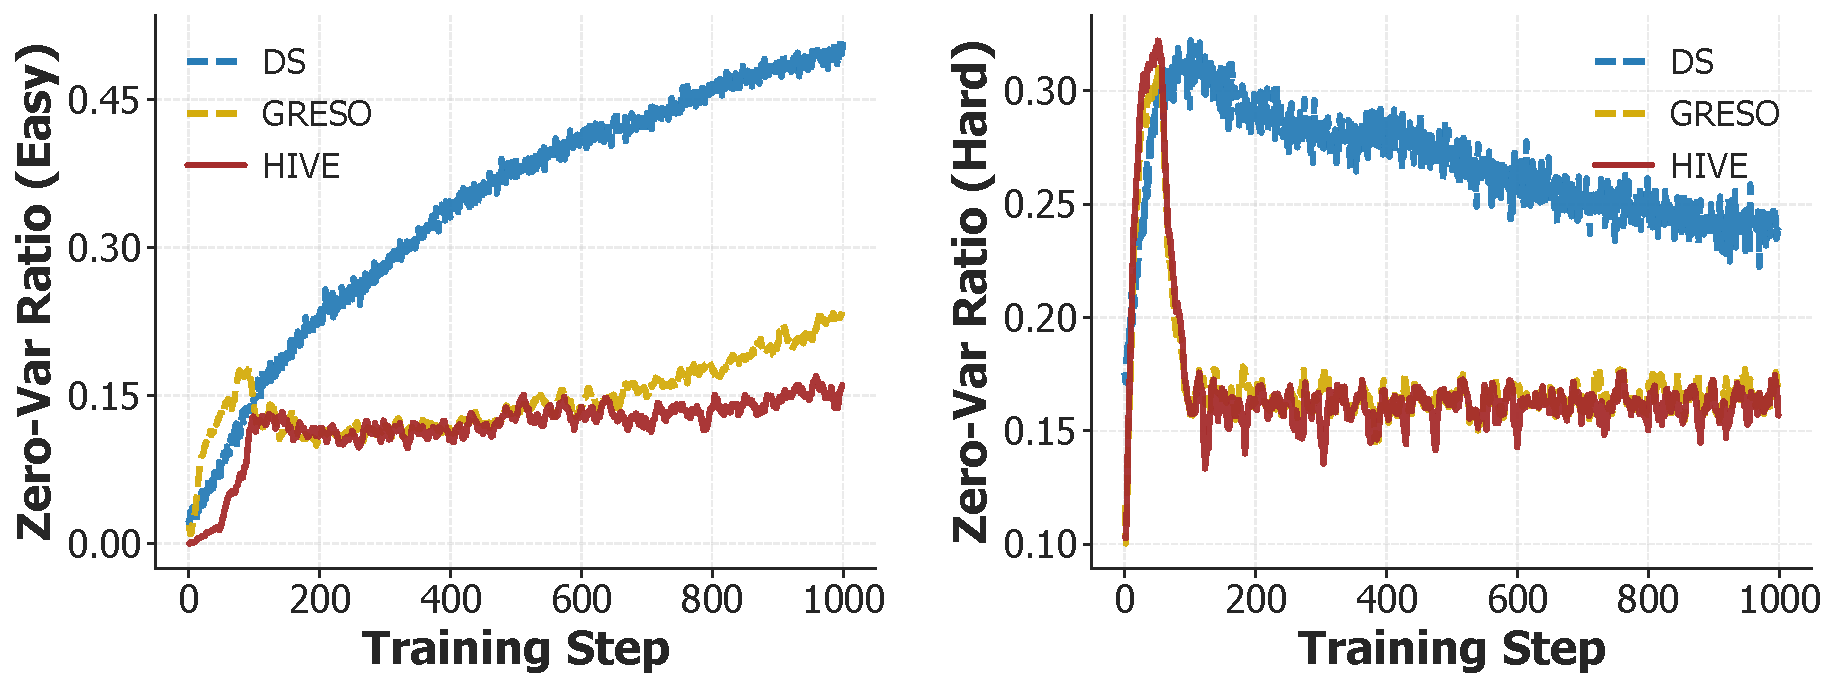
\includegraphics[width=\textwidth,trim=0 0 440.4bp 0,clip]{figures/experiment/fig6-zerovar-easy-hard-polished.pdf}
        \caption{Easy zero-variance}
        \label{fig:zerovar_easy}
    \end{subfigure}
    \hfill
    \begin{subfigure}[b]{0.24\textwidth}
        \centering
        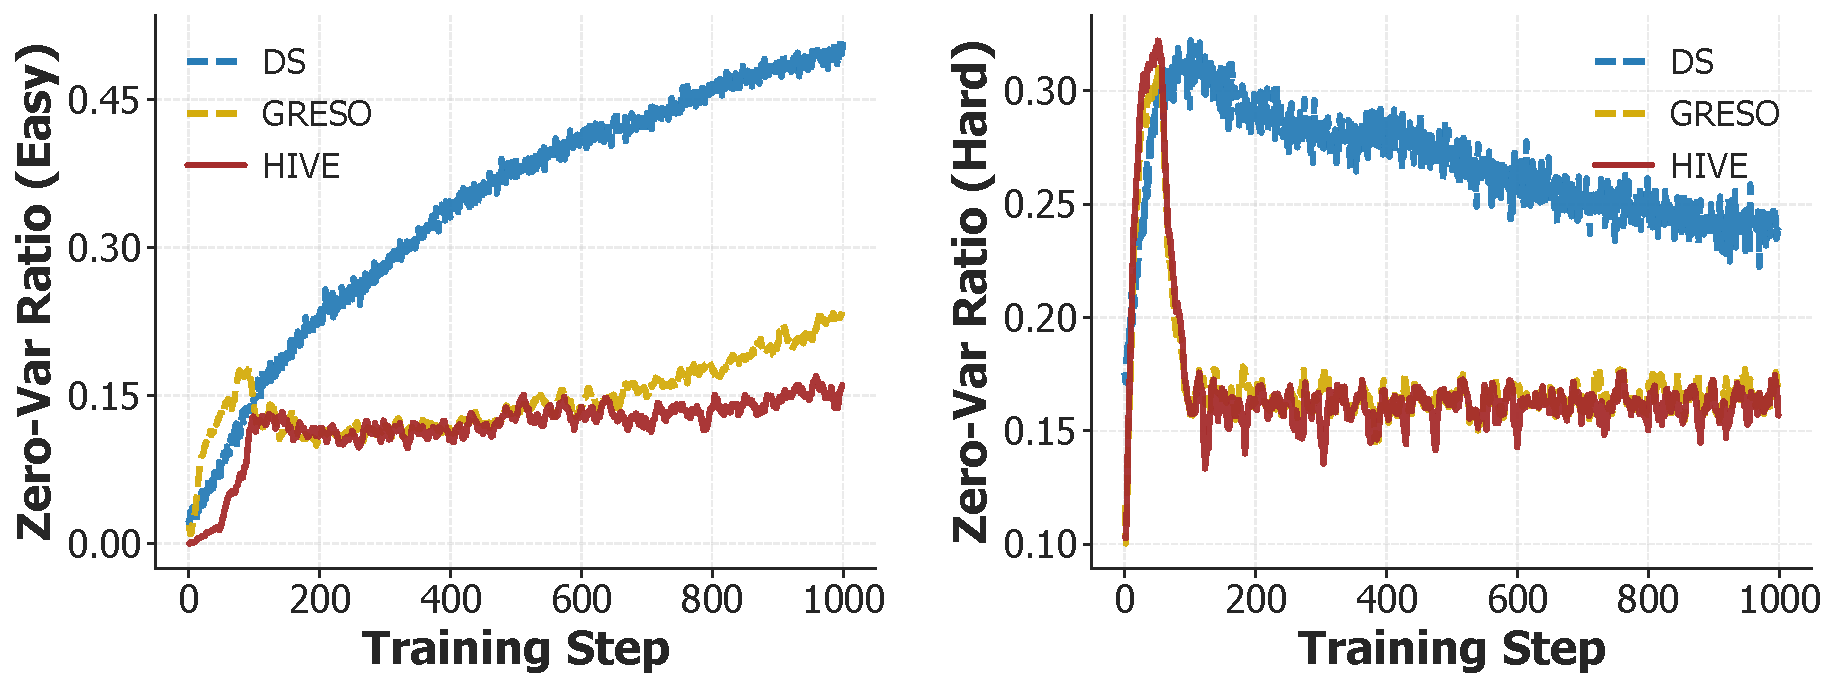
\includegraphics[width=\textwidth,trim=440.4bp 0 0 0,clip]{figures/experiment/fig6-zerovar-easy-hard-polished.pdf}
        \caption{Hard zero-variance}
        \label{fig:zerovar_hard}
    \end{subfigure}
    \hfill
    \begin{subfigure}[b]{0.24\textwidth}
        \centering
        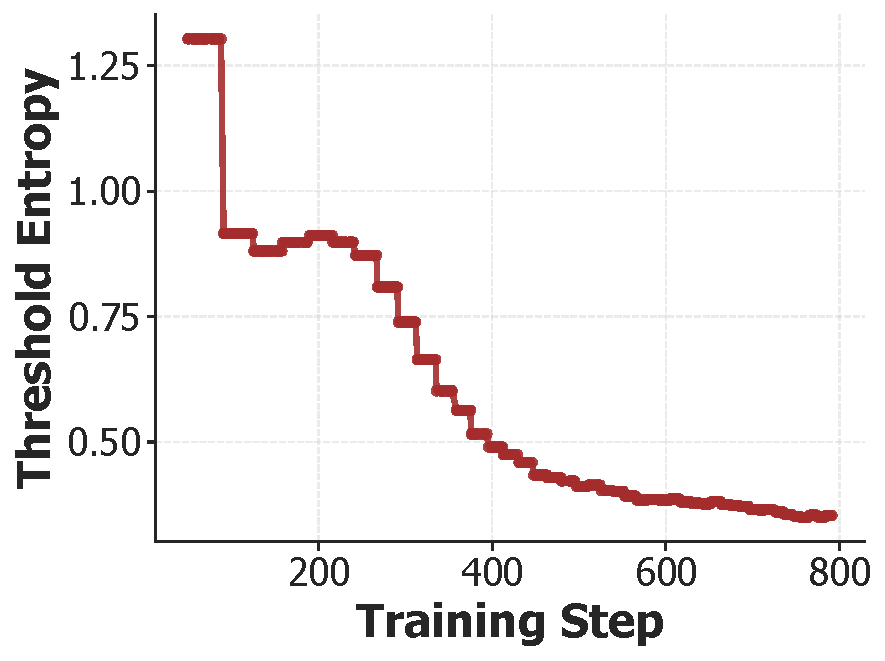
\includegraphics[width=\textwidth]{figures/experiment/fig6-gamma-entropy-polished.pdf}
        \caption{Entropy threshold}
        \label{fig:gamma_entropy}
    \end{subfigure}
    \hfill
    \begin{subfigure}[b]{0.24\textwidth}
        \centering
        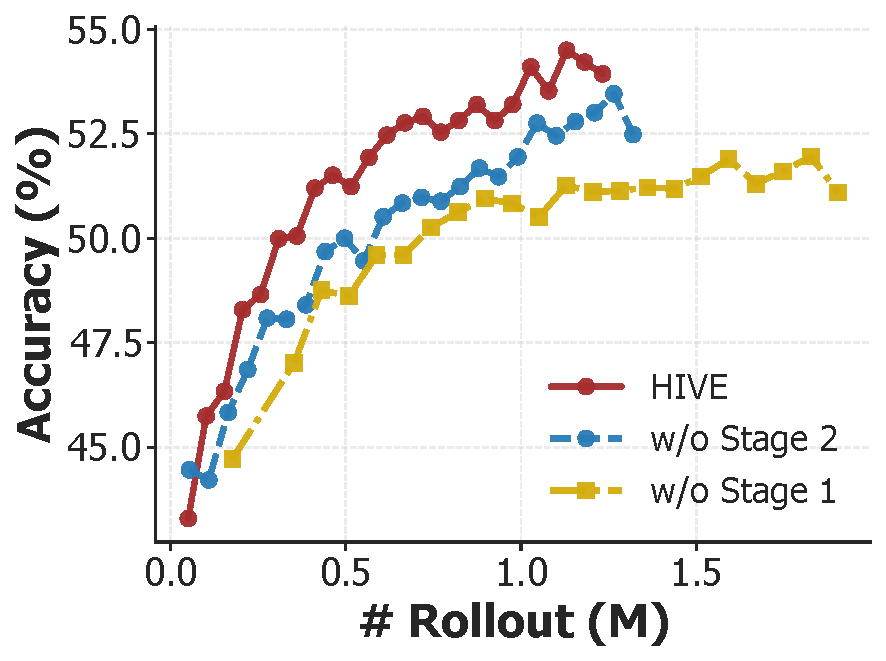
\includegraphics[width=\textwidth]{figures/experiment/fig6-stage-ablation-polished.pdf}
        \caption{Stage ablation}
        \label{fig:ablation}
    \end{subfigure}

    \caption{\textbf{Zero-variance ratios and component analysis.}
    (a)~Easy zero-variance ratio: HIVE keeps the lowest fraction of all-correct prompts throughout training.
    (b)~Hard zero-variance ratio: HIVE rapidly drops below DS and tracks GRESO.
    (c)~The Stage~2 median prompt-entropy threshold $\gamma$ adapts as the policy becomes more confident.
    (d)~Removing either Stage~1 or Stage~2 worsens the accuracy--rollout tradeoff.}%
    \label{fig:non-zero-diveregence-comparison}
    \vskip -0.08in
\end{figure*}

\best{HIVE rejects stale zero-variance prompts as training evolves.}
The zero-variance ratio measures how often selected prompts produce no informative gradient. Figures~\ref{fig:zerovar_easy} and~\ref{fig:zerovar_hard} show that DS wastes a large fraction of rollouts on easy zero-variance prompts as the model improves, while GRESO remains vulnerable to stale historical records. HIVE maintains a lower zero-variance ratio for both easy and hard prompts, indicating that online verification helps track the moving edge rather than relying on outdated metadata.

\subsection{Component Study: Why Both Stages Matter}
\label{subsec:exp-component-study}

\best{The entropy gate adapts with the current policy.}
Figure~\ref{fig:gamma_entropy} tracks the Stage~2 median threshold $\gamma$, which decreases as the model becomes more confident. This behavior is expected: as the policy improves, the prompt-side uncertainty distribution shifts, and a fixed threshold would either over-prune or admit stale prompts. The median gate keeps the verification rule relative to the current candidate pool. 
\best{The two-stage decomposition is necessary.}
Figure~\ref{fig:ablation} compares the full HIVE pipeline with variants that remove either stage. Without Stage~2, HIVE loses online precision and becomes more vulnerable to stale metadata. Without Stage~1, the verifier receives too many low-value candidates, reducing efficiency. The full method gives the best accuracy--rollout tradeoff, supporting the decomposition into efficient historical narrowing followed by online verification.

\section{Related Work}
\label{sec:related-work}

\textbf{RLVR for LLM reasoning.}
Reinforcement learning is a standard post-training tool for aligning and improving LLMs~\cite{christiano2017deep,bai2022training,ouyang2022training,rafailov2023direct}. Recent reasoning systems increasingly rely on reinforcement learning with verifiable rewards (RLVR), where correctness can be checked directly for tasks such as mathematics and code~\cite{guo2025deepseek,hu2025reinforce++,liu2503understanding,jaech2024openai,Zhang2025SRPOAC}. Algorithmic work improves this training loop through value-enhanced PPO variants such as VC-PPO~\cite{yuan2025s} and VAPO~\cite{yue2025vapo}, group-based methods such as RLOO~\cite{ahmadian2024back} and GRPO~\cite{shao2024deepseekmath}, replay-based updates~\cite{liang2025squeeze,li2025repo,zhang2025rlep}, and objective modifications such as Dr. GRPO~\cite{liu2503understanding} and GSPO~\cite{zheng2025group}. These methods improve optimization stability or sample reuse, but they do not directly solve the pre-rollout allocation problem studied here: which prompts deserve expensive response generation at the current training step.

\textbf{Prompt selection and data-efficient RL training.}
Data curation is essential for efficient LLM training. Offline filtering methods rank prompts before training using quality, difficulty, diversity, or scale heuristics~\cite{Wang2025ReinforcementLF,Fatemi2025ConciseRV,Li2025LIMRLI,shi2025efficient,tang2025towards,zhou2023lima,ye2025limo}. They are efficient once training begins, but they are policy-agnostic and cannot adapt as the model's competence changes. Rollout-based online methods, including Dynamic Sampling in DAPO~\cite{yu2025dapo} and related online down-sampling or difficulty-filtering approaches~\cite{meng2025mm,foster2025learning,xu2025not,lin2025cppo,sun2025efficient,bae2025online}, are more precise because they observe current rewards, but they require the rollouts they aim to save. History-based and estimator-based approaches such as GRESO~\cite{zheng2025act}, Bayesian task selection~\cite{chen2025self,zeng2025cures,shen2025bots}, and curriculum estimators use past trajectories or uncertainty models to reduce selection cost, but their estimates can become stale in a changing policy environment. Auxiliary-model methods such as DOTS~\cite{sun2025dots} and PCL~\cite{Gao2025PCL} add external or on-policy predictors for difficulty, improving adaptivity at the cost of additional compute or memory.

Overall, prior methods face limitations in online and efficient prompt selection. HIVE differs by explicitly decomposing the problem into history-informed coarse narrowing and prompt-side online verification, allowing it to retain the efficiency of historical filtering while correcting stale metadata before rollout. Detailed related work is provided in Appendix~\ref{appendix-sec:detailed_related_work}.

\section{Conclusion}
RLVR prompt selection is best understood as a moving-edge tracking problem. Useful prompts are not merely those that look difficult or uncertain in isolation; they are prompts that remain informative for the current policy. HIVE efficiently identify those prompts with a dual-stage mechanism: history-informed narrowing reduces the candidate pool, and prompt-side online verification filters stale candidates under the current model. Across math reasoning benchmarks and model scales, HIVE reduces rollout and training cost while preserving or improving final accuracy.

\section{Limitations and Broader Impacts}
\label{sec:limitations}
% \red{re-write Limitations. }
% Our evaluation does not include prompt-side verification to multimodal RLVR. HIVE also introduces hyperparameters such as $\lambda$, $\Delta p$, and the target zero-variance ratio $\alpha$; although the adaptive mechanism reduces manual tuning, we have not exhaustively searched these settings across all model scales. Finally, due to the cost of large-scale RLVR, the current main results do not include repeated-run error bars or oracle high-gradient precision/recall measurements. We instead report rollout cost, zero-variance ratios, prompt--response entropy correlation, and component ablations as mechanism evidence.
% \section*{Impact Statements}
% \red{need more negilible limitations}. This paper presents work whose goal is to advance the field of machine learning. HIVE has the potential to improve the data and computational efficiency of reinforcement learning for large reasoning models. By reducing unnecessary rollouts, it can lower the energy cost and carbon footprint of RL post-training. Lower compute requirements may also make advanced model fine-tuning more accessible to academic groups with limited resources. We do not foresee specific negative societal consequences beyond the general risks associated with improving LLM reasoning capabilities.
\paragraph{Limitations.} 
% The rank-consistency analysis provides a conservative sufficient condition for prompt-side entropy to serve as an online verifier, rather than a tight guarantee for all individual prompt pairs. Its worst-case concentration arguments may lead to loose margins for modern LRMs. This limitation does not affect HIVE's main contribution or empirical conclusions, since HIVE only requires prompt-side entropy to act as a useful low-cost signal for filtering stale candidates, which is supported by our entropy analysis, ablations, and end-to-end efficiency gains. Deriving tighter variance-dependent guarantees is left for future work.
Our rank-consistency analysis is intended as a conservative sufficient condition for using prompt-side entropy as an online verifier, rather than a tight characterization of every empirical prompt pair. The proof uses worst-case concentration and bounded-approximation arguments, which may yield loose margins for modern LRMs. This does not affect HIVE's algorithmic design or empirical conclusions, as the method does not rely on exact prompt-level ranking; it only requires prompt-side entropy to provide a useful low-cost signal for filtering stale candidates. This role is validated by our prompt--response entropy analysis, component ablations, and end-to-end efficiency gains. Tighter variance-dependent guarantees remain an interesting direction for future work.
\paragraph{Broader impacts.} 
HIVE improves the efficiency of RL post-training by reducing unnecessary rollouts, thereby lowering training cost, energy consumption, and carbon footprint. This may make RLVR-style post-training more accessible to resource-constrained research groups. We do not foresee specific negative societal impacts beyond the general risks associated with stronger LLM capabilities.
% HIVE aims to improve the computational efficiency of RL post-training for large reasoning models. By reducing unnecessary rollouts, it can lower training cost, energy consumption, and carbon footprint, while making RLVR-style post-training more accessible to resource-constrained research groups. We do not foresee specific negative societal impacts beyond the general risks associated with stronger LLM reasoning capabilities
% \red{need check if the fake references exists.}
% \red{examine the checklist}

\bibliographystyle{plainnat}
\bibliography{references}

\clearpage
\appendix
\section*{Appendix}
In this appendix, we provide the rank-consistency analysis for Theorem~\ref{thm:ranking-informal} (Appendix~\ref{appendix-sec:proof-thm}), experimental settings (Appendix~\ref{appendix-sec:detailed-experimental-setting}), preliminary-study details (Appendix~\ref{sec:preliminary-setup}), detailed related work (Appendix~\ref{appendix-sec:detailed_related_work}), additional experiments (Appendix~\ref{appendix-sec:additional-exp}), the HIVE algorithm (Appendix~\ref{appendix-sec:alg}), and asset liciences (Appendix~\ref{sec:asset-licenses}).

% \red{Need to add more details on the experiment settings.}
\section{Rank-Consistency Analysis for Theorem~\ref{thm:ranking-informal}}
\label{appendix-sec:proof-thm}
This section provides a rank-consistency justification for using prompt-side entropy $V(x)$ as a low-cost proxy for response-side entropy $U^*(x)$. The result is meant to formalize the intuition behind Stage~2 under simplifying assumptions; the main empirical support for HIVE comes from the correlation and ablation results reported in the paper.

\subsection{Preliminaries and Notations}
Let the fixed model parameters be $\thetahat$ and the vocabulary size be $|\Vcal|$. We denote the sampling policy used for generation as $q(\cdot|x)$ (e.g., temperature sampling with parameter $\tau$).

\paragraph{Observable: Prompt-side Entropy.} 
Given a prompt sequence $x = (x_1, \dots, x_L)$, the model computes the probability distribution over the vocabulary at each position. Let $p_{\thetahat, \tau}(\cdot|x_{<l}) = \text{softmax}(z_{\thetahat}(x_{<l})/\tau)$ denote the temperature-scaled probability. The observable token entropy at position $l$ is $e_l(x) := \mathcal{H}(p_{\thetahat, \tau}(\cdot|x_{<l}))$. We define the aggregated prompt entropy as:
\begin{equation}
  V(x) := \frac{1}{L-1}\sum_{l=2}^{L} e_l(x).
\end{equation}
% Note that $V(x)$ is fully deterministic given the model and the prompt.

\paragraph{Observable: Response-side Entropy.} 
For a given prompt $x$, we generate $G$ independent rollouts to estimate the output entropy. For the $r$-th rollout, let the response be $y^{(r)}_{1:L_r}$. Define the step context as $c_t^{(r)} := (x, y_{<t}^{(r)})$. The token entropy at step $t$ is $u_t^{(r)}(x) := \mathcal{H}(p_{\thetahat, \tau}(\cdot|c_t^{(r)}))$. 
The length-normalized entropy for rollout $r$ is $U^{(r)}(x) := \frac{1}{L_r}\sum_{t=1}^{L_r} u_t^{(r)}(x)$.
The final empirical estimator is the average over $n$ rollouts:
\begin{equation}
  \hat{U}(x) := \frac{1}{n}\sum_{r=1}^{n} U^{(r)}(x).
\end{equation}
We define the target $U^*(x) := \mathbb{E}_{y \sim q(\cdot|x)}[U^{(r)}(x)]$ as the expected entropy under the sampling policy.

\subsection{Theoretical Bridges and Assumptions}
\label{subsec:thm-theoretical-proof}
To bridge the gap between the computationally tractable token-level logits entropy and the model's high-level semantic entropy, we establish our theoretical analysis upon two pivotal assumptions. First, we map the observable token entropy to the model's internal representation entropy (\textit{Representation Approximation}). Second, we posit that this internal entropy propagates linearly from the prompt to the response (\textit{Entropy Propagation}).

\subsubsection{From Token to Representation.}
While observable entropies $V(x)$ and $U^*(x)$ are derived from the final output layer, true epistemic entropy is often better encoded in the latent space. Following \cite{flue2025}, we define the \textit{Representation Entropy} $s(c)$ as the entropy of hidden states at a deep layer $b \approx N$, formally $s(c) \approx \hat{\mathcal{H}}[H^{(b)}|c]$. We define the aggregated representation entropies for the prompt and response as:
\begin{equation}
\begin{split}
    S_{\text{prompt}}(x) := \frac{1}{L-1}\sum_{l=2}^L s(x_{<l}),\;
    S_{\text{resp}}(x) := \mathbb{E}_{y} \left[\frac{1}{T}\sum_{t=1}^{T} s(c_t)\right].
\end{split}
\end{equation}

Based on this definition, we introduce our first assumption to link observables to internal states.

\begin{assumption}[Representation Approximation]
\label{ass:representation}
The observable token entropy approximates the internal representation entropy up to a small residual $\delta$:
\begin{equation}
  |V(x) - S_{\text{prompt}}(x)| \le \delta \quad \text{and} \quad |U^*(x) - S_{\text{resp}}(x)| \le \delta.
\end{equation}
\end{assumption}
\noindent\textit{{Justification (Theoretical):}} This assumption is grounded in Proposition 1 of \cite{flue2025}, which proves that for trained LLMs, the entropy of hidden states in deep layers serves as an approximate upper bound for the predictive posterior entropy (i.e., our token entropy). As the layer depth $b \to N$, the mutual information is maximized, ensuring the token entropy is tightly correlated with the internal representation.

% \subsubsection{Entropy Propagation.}
% Having established the link to internal representations, we next model how this entropy evolves from the input context to the generation phase.

% \begin{assumption}[Entropy Propagation]
% \label{ass:propagation}
% The representation entropy in the prompt propagates linearly to the response generation stage. There exist constants $a > 0, b \in \mathbb{R}$ such that:
% \begin{equation}
%   |S_{\text{resp}}(x) - (a S_{\text{prompt}}(x) + b)| \le \epsilon.
% \end{equation}
% \end{assumption}

% % \begin{figure}[t]
    \centering
    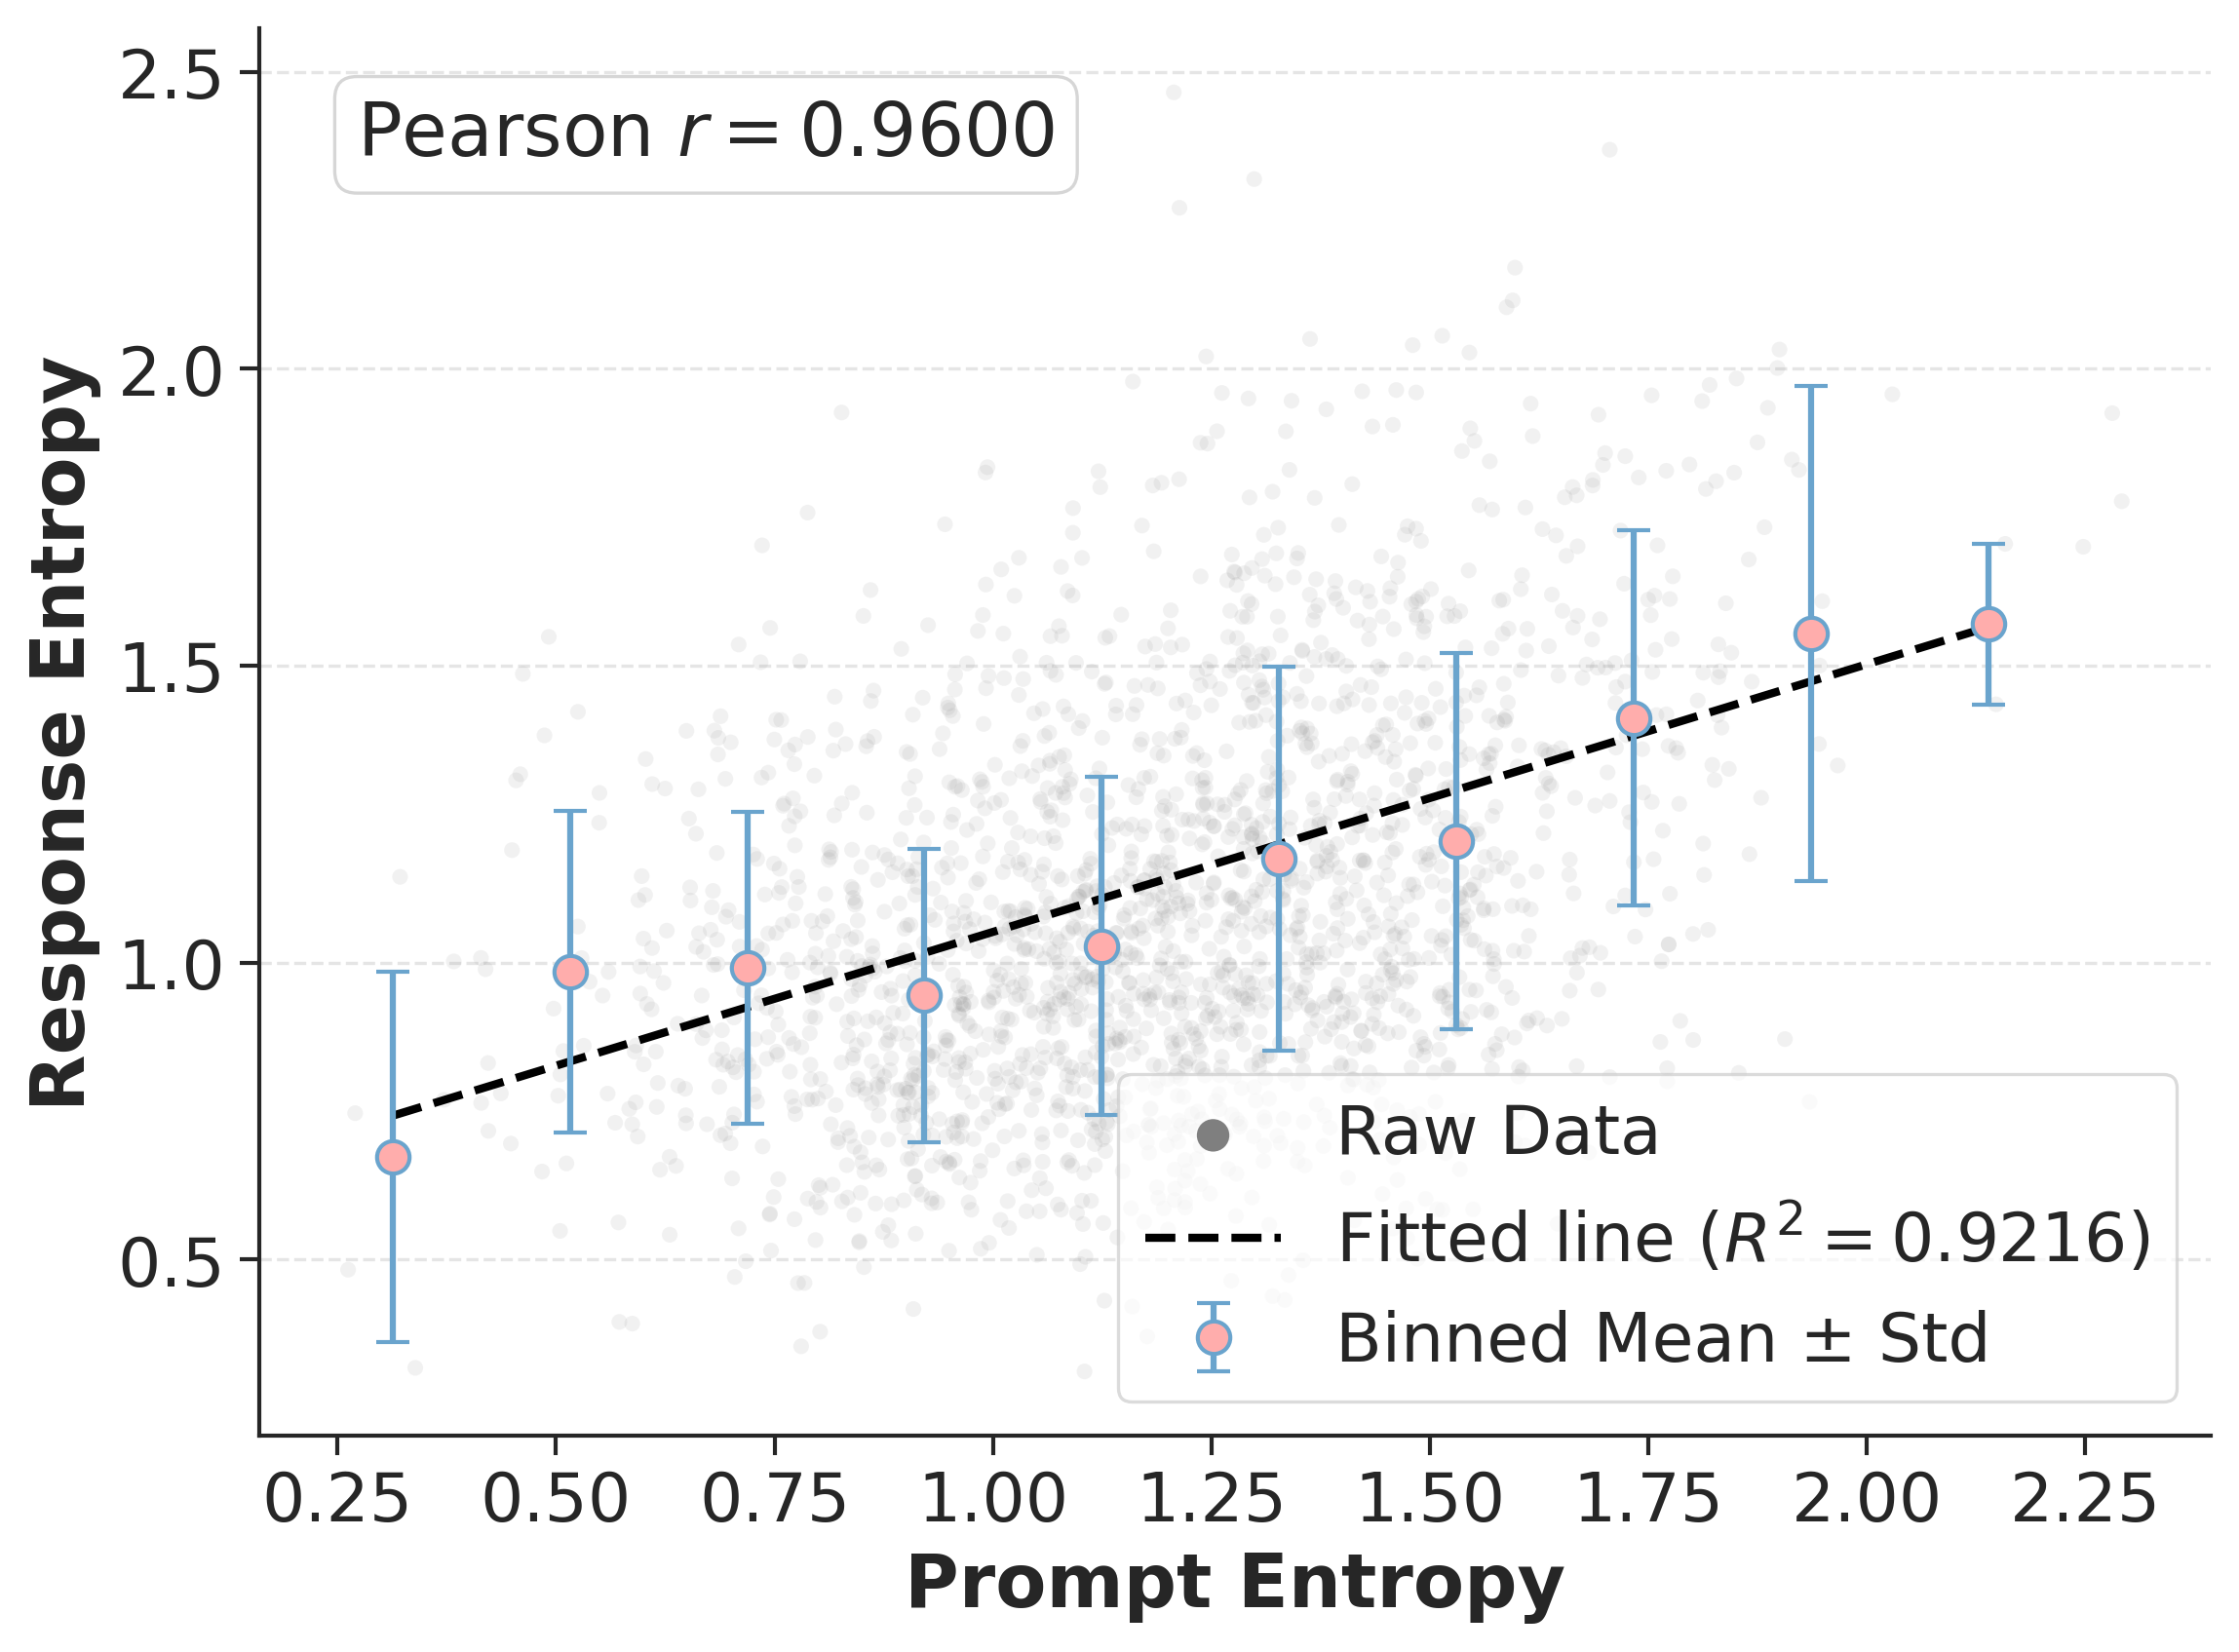
\includegraphics[width=\linewidth]{figures/appendix/binned_mean_respRatio15-beauty.png}
    \captionof{figure}{\textbf{Empirical support for entropy propagation (Assumption~\ref{ass:propagation}).} The scatter plot shows the relationship between prompt mean entropy and response entropy over 2,048 samples. We report binned statistics (blue points, mean $\pm$ std) to separate the average trend from sample-level generation noise (grey dots). The regression line on the binned data has $R^2=0.9216$ and Pearson $r=0.9600$, supporting prompt-side entropy as a response-side entropy proxy.}%By focusing on the top-tier entropy tokens, we capture the propagation of semantic uncertainty as characterized by \cite{wang2025beyond}.
    \label{fig:entropy_correlation}
    % \vspace{-3mm} % 可选：微调Caption与正文之间的距离，节省空间
% \end{figure}

\noindent % 防止首行缩进造成未对齐
\subsubsection{Entropy Propagation.}

% --- 开始 Wrapfigure 环境 ---
% {r} 表示靠右，{0.45\textwidth} 是图片区域宽度，可根据需要调整
\begin{wrapfigure}{r}{0.45\textwidth} 
    \vspace{-20pt} % 【调整核心】向上移动图片，使其与左侧标题/正文顶部对齐
    \centering
    
    % 这里插入你的图片内容
    % 注意：被 input 的文件内不能有 \begin{figure} 环境，只能有纯图片代码
    % \begin{figure}[t]
    \centering
    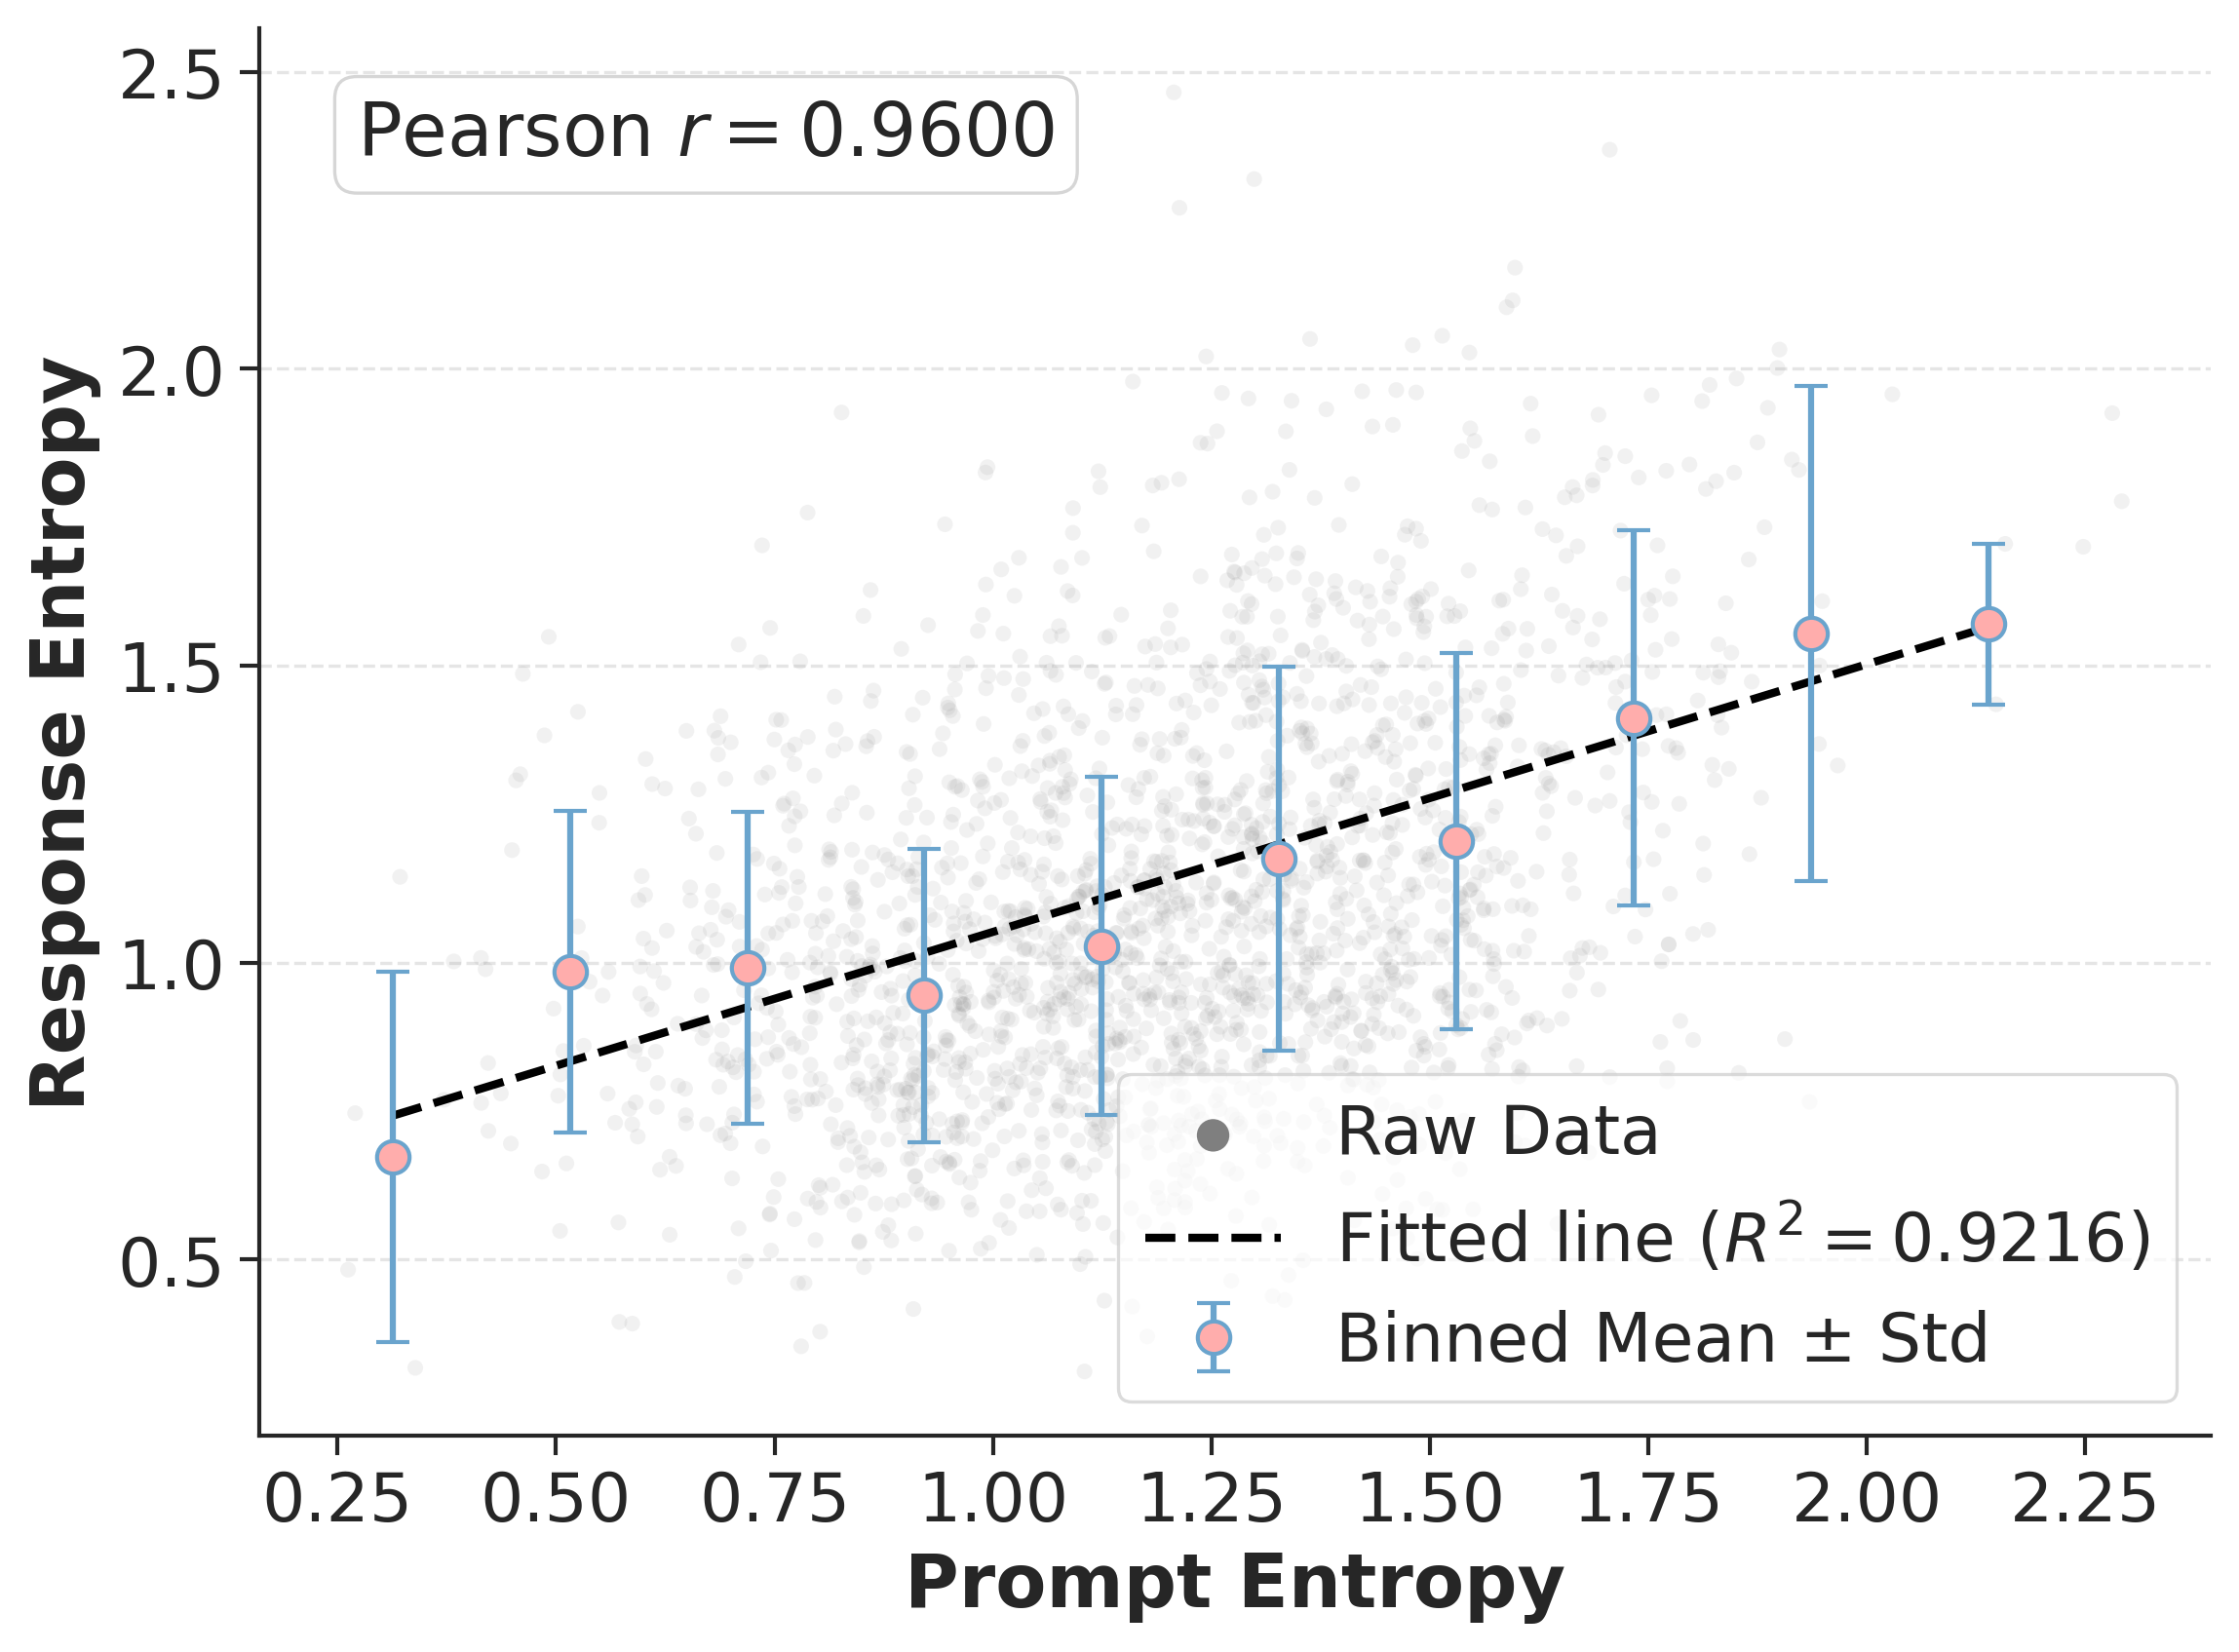
\includegraphics[width=\linewidth]{figures/appendix/binned_mean_respRatio15-beauty.png}
    \captionof{figure}{\textbf{Empirical support for entropy propagation (Assumption~\ref{ass:propagation}).} The scatter plot shows the relationship between prompt mean entropy and response entropy over 2,048 samples. We report binned statistics (blue points, mean $\pm$ std) to separate the average trend from sample-level generation noise (grey dots). The regression line on the binned data has $R^2=0.9216$ and Pearson $r=0.9600$, supporting prompt-side entropy as a response-side entropy proxy.}%By focusing on the top-tier entropy tokens, we capture the propagation of semantic uncertainty as characterized by \cite{wang2025beyond}.
    \label{fig:entropy_correlation}
    % \vspace{-3mm} % 可选：微调Caption与正文之间的距离，节省空间
% \end{figure}

    
    % 如果你的 input 文件里没有 caption，请在这里加：
    % \caption{Validation of Entropy Propagation...}
    % \label{fig:entropy_correlation}
    
    \vspace{-10pt} % 减少图片下方的空白
\end{wrapfigure}
% --- 结束 Wrapfigure 环境 ---

% 左侧的文字会自动填充在图片左边
Having established the link to internal representations, we next model how this entropy evolves from the input context to the generation phase.

\begin{assumption}[Entropy Propagation]
\label{ass:propagation}
The representation entropy in the prompt propagates linearly to the response generation stage. There exist constants $a > 0, b \in \mathbb{R}$ such that:
\begin{equation}
  |S_{\text{resp}}(x) - (a S_{\text{prompt}}(x) + b)| \le \epsilon.
\end{equation}
\end{assumption}

% 当文字长度超过图片高度时，下方的文字会自动变宽，填满图片下方的空白
\noindent\textit{{Justification (Empirical):}} To examine this linearity and quantify the noise $\epsilon$, we analyzed 2,048 prompts. We computed $V(x)$ as the proxy for $S_{\text{prompt}}$ (per Assumption~\ref{ass:representation}). %For the response side, to capture effective semantic entropy and avoid dilution by low-entropy functional tokens, we applied a \textit{High-Entropy Filtering} strategy (averaging the top 15\% entropy tokens across 8 rollouts). This strategy aligns with findings in~\cite{wang2025beyond}, who demonstrates that reasoning is driven by a ``high-entropy minority" of tokens (``forks"). 
To mitigate the intrinsic stochasticity of LLM generation, we use a binned analysis. As shown in Figure~\ref{fig:entropy_correlation}, prompt-side and response-side entropy have a strong positive correlation (Pearson $r$=0.9600). The binned mean trend is well approximated by a line with $R^2=0.9216$, supporting the linear structure in Assumption~\ref{ass:propagation} for the regimes studied here.

\subsection{Concentration Bound}
\begin{lemma}[High-probability Concentration]
\label{lemma:concentration}
For any fixed prompt $x$ and tolerance $\eta > 0$, the empirical entropy $\hat{U}(x)$ concentrates around the true expectation $U^*(x)$:
\begin{equation}
  \Pr\left(|\hat{U}(x) - U^*(x)| > \eta\right) \le 2 \exp\left( - \frac{2n\eta^2}{(\log|\Vcal|)^2} \right).
  \label{eq:concentration_prob}
\end{equation}
Consequently, for any confidence level $1-\alpha$ (where $\alpha \in (0, 1)$), with probability at least $1-\alpha$:
\begin{equation}
  |\hat{U}(x) - U^*(x)| \le \eta(\alpha) := \log|\Vcal| \sqrt{\frac{\log(2/\alpha)}{2n}}.
  \label{eq:concentration_bound}
\end{equation}
\end{lemma}

\begin{proof}
The sequence-level entropy $U^{(r)}(x)$ for each rollout is bounded within $[0, \log|\Vcal|]$. Since the $G$ rollouts are generated independent and identically distributed (i.i.d.) from the sampling policy $q(\cdot|x)$, Hoeffding's inequality~\cite{hoeffding1963probability} applies directly to the empirical mean $\hat{U}(x)$, yielding the stated bound.
\end{proof}

\subsection{Main Result: Rank Consistency}

\begin{theorem}[Theorem~\ref{thm:ranking-informal}]
\label{thm:ranking-appendix}
Consider a pair of prompts $(x, x')$. Let $\Delta_V := V(x) - V(x')$ be the observable difference in prompt entropy, and $\Delta_U := \hat{U}(x) - \hat{U}(x')$ be the difference in estimated response entropy. Under Assumptions \ref{ass:representation} and \ref{ass:propagation}, for any $\alpha \in (0, 1)$, with probability at least $1-2\alpha$:
\begin{equation}
  |\Delta_U - a\Delta_V| \le 2\epsilon + 2(a+1)\delta + 2\eta(\alpha).
  \label{eq:theorem_bound-appendix}
\end{equation}
Crucially, if the prompt entropy margin satisfies $|a\Delta_V| > 2\epsilon + 2(a+1)\delta + 2\eta(\alpha)$, then the ranking is preserved:
\begin{equation}
  \text{sign}(\hat{U}(x) - \hat{U}(x')) = \text{sign}(V(x) - V(x')).
  \label{eq:theorem_order-appendix}
\end{equation}
\end{theorem}

\begin{proof}
We decompose the error into three components: sampling noise, propagation residual, and representation approximation error.

\noindent\textbf{Step 1: Sampling Noise.} By applying Lemma \ref{lemma:concentration} and a union bound over prompts $x$ and $x'$, with probability $\ge 1-2\alpha$, the empirical estimates are close to their true expectations:
\begin{equation}
  |\Delta_U - (U^*(x) - U^*(x'))| \le 2\eta(\alpha).
  \label{eq:step1}
\end{equation}

\noindent\textbf{Step 2: Propagation Dynamics.} From Assumption \ref{ass:propagation}, we express the response representation entropy as $S_{\text{resp}}(x) = a S_{\text{prompt}}(x) + b + \xi(x)$ where $|\xi(x)| \le \epsilon$. The difference between two prompts cancels out the bias term $b$:
\begin{equation}
  |(S_{\text{resp}}(x) - S_{\text{resp}}(x')) - a(S_{\text{prompt}}(x) - S_{\text{prompt}}(x'))| \le 2\epsilon.
  \label{eq:step2}
\end{equation}

\noindent\textbf{Step 3: Representation Approximation.} Using Assumption \ref{ass:representation}, we substitute the theoretical representation entropies with observable token entropies. We have $|(U^*(x) - U^*(x')) - (S_{\text{resp}}(x) - S_{\text{resp}}(x'))| \le 2\delta$ and $|(S_{\text{prompt}}(x) - S_{\text{prompt}}(x')) - \Delta_V| \le 2\delta$. 
Applying the triangle inequality and scaling the prompt-side error by $a$:
\begin{equation}
  |(U^*(x) - U^*(x')) - a\Delta_V| \le 2\epsilon + 2\delta + 2a\delta = 2\epsilon + 2(a+1)\delta.
  \label{eq:step3}
\end{equation}

Combining Eq. \eqref{eq:step1} and Eq. \eqref{eq:step3} yields the final bound in Eq. \eqref{eq:theorem_bound-appendix}. The condition $|a\Delta_V| > \text{RHS}$ (Right-Hand Side) ensures that the signal magnitude exceeds the worst-case cumulative noise, guaranteeing that the sign of the difference remains unchanged.
\end{proof}

% \section{Detailed Experimental Setting for Main Study}
% \label{appendix-sec:detailed-experimental-setting}

% We mainly follow the experimental protocol of GRESO~\cite{zheng2025act}.

% \textbf{Models and datasets.} We evaluate Qwen2.5-Math-1.5B~\cite{yang2024qwen25mathtechnicalreportmathematical}, DeepSeek-R1-Distill-Qwen-1.5B~\cite{guo2025deepseek}, Qwen3-4B-Base~\cite{yang2025qwen3technicalreport}, Qwen2.5-Math-7B~\cite{yang2024qwen25mathtechnicalreportmathematical}, and Llama-3.2-3B-Instruct~\cite{grattafiori2024llama3}. We additionally evaluate Qwen2.5-14B/32B~\cite{qwen2.5-large} in the scaling study. We set the context length to 4096 for Qwen2.5-Math-1.5B/7B, 8192 for DeepSeek-R1-Distill-Qwen-1.5B, Qwen3-4B-Base, and Llama-3.2-3B-Instruct, and 16384 for Qwen2.5-14B/32B. The training datasets are: (1) DAPO+MATH, the combination of DAPO~\cite{yu2025dapo} and MATH~\cite{hendrycks2021measuringmathematicalproblemsolving}; and (2) a 30,000-example Open-R1 math subset~\cite{openr1}.

% \textbf{Training.} Our implementation is based on verl~\cite{verl2025} and vLLM~\cite{vLLM2023SOSP}. We train all main models on 8$\times$A100 GPUs and set the rollout sampling temperature to 1.0. For Qwen2.5-Math-1.5B/7B, Qwen3-4B-Base, and Llama-3.2-3B-Instruct, the training batch size is 256, rollout sampling batch size is 384, and mini-batch size is 512. For DeepSeek-R1-Distill-Qwen-1.5B, the training batch size is 128, rollout sampling batch size is 192, and mini-batch size is 512. We sample $G=8$ responses per prompt. All models are trained for 1000 steps with AdamW~\cite{loshchilov2018decoupled}, learning rate $10^{-6}$, $\beta_1=0.9$, $\beta_2=0.999$, and weight decay 0.01. Similar to~\citet{yu2025dapo}, we remove the KL-divergence term. The actor is trained with Fully Sharded Data Parallel (FSDP)~\citep{zhao2023pytorch}.

% \textbf{Baselines and budgets.} We compare HIVE with four prompt-selection baselines. Dynamic Sampling (DS)~\cite{yu2025dapo} performs rollout-based online filtering and serves as the full-cost online baseline. Pre-filter is a fixed offline selector: prompts are filtered before RL training and the selected subset remains unchanged during policy updates. GRESO~\cite{zheng2025act} is a history-based selector using past reward trajectories. PCL~\cite{Gao2025PCL} uses an auxiliary prompt-curriculum selector. For each model family, GRESO, Pre-filter, and PCL are run under the same rollout budget shown in Table~\ref{tab:main_comparison}. Since the original PCL paper evaluates Pre-filter and PCL by training until a fixed wall-clock budget, which differs from our 1000-step comparison protocol, we run these two baselines twice under the matched rollout count: one run follows the original PCL-paper settings, and the other follows our common settings. We report the higher average benchmark score across the two runs. Selector-specific overhead is included in the ``Other'' column of Table~\ref{tab:efficiency_cost}.

% \textbf{Rewards and evaluation.} For reward assignment, we give a score of 0.1 when an answer can be successfully extracted and 1.0 when the extracted answer is correct. We evaluate every 50 steps on Math500~\cite{hendrycks2021measuringmathematicalproblemsolving}, AIME24~\cite{aops2024aime}, AMC~\cite{aops2024amc}, Minerva Math~\cite{NEURIPS2022_18abbeef}, Gaokao~\cite{zhang2024gaokao}, and Olympiad Bench~\cite{he-etal-2024-olympiadbench}. Following~\citet{zheng2025act}, we report the checkpoint with the best average performance on the six benchmarks.

% \begin{tcolorbox}[myexample={Question Template}]
% Please solve the following math problem: \{\{Question Description\}\}. The assistant first thinks about the reasoning process step by step and then provides the user with the answer. Return the final answer in \textbackslash boxed\{\} tags, for example \textbackslash boxed\{1\}. Let's solve this step by step.
% \end{tcolorbox}
\section{Detailed Experimental Setting for Main Study}
\label{appendix-sec:detailed-experimental-setting}

This section gives the full experimental protocol for the main study. We follow the general setup of GRESO~\cite{zheng2025act} and make three aspects explicit: the shared training and evaluation protocol, the budget-matched baseline comparison, and the HIVE-specific selector configuration.

\subsection{Shared Training and Evaluation Protocol}
\label{appendix-subsec:shared-exp-protocol}

\paragraph{Models and datasets.}
We evaluate Qwen2.5-Math-1.5B~\cite{yang2024qwen25mathtechnicalreportmathematical}, DeepSeek-R1-Distill-Qwen-1.5B~\cite{guo2025deepseek}, Qwen3-4B-Base~\cite{yang2025qwen3technicalreport}, Qwen2.5-Math-7B~\cite{yang2024qwen25mathtechnicalreportmathematical}, and Llama-3.2-3B-Instruct~\cite{grattafiori2024llama3}. We additionally evaluate Qwen2.5-14B/32B~\cite{qwen2.5-large} in the scaling study. The context length is 4096 for Qwen2.5-Math-1.5B/7B, 8192 for DeepSeek-R1-Distill-Qwen-1.5B, Qwen3-4B-Base, and Llama-3.2-3B-Instruct, and 16384 for Qwen2.5-14B/32B. Training uses two math-reasoning corpora: DAPO+MATH, which combines DAPO~\cite{yu2025dapo} and MATH~\cite{hendrycks2021measuringmathematicalproblemsolving}, and a 30,000-example Open-R1 math subset~\cite{openr1}.

\paragraph{Optimization and rollout.}
Our implementation is based on verl~\cite{verl2025} and vLLM~\cite{vLLM2023SOSP}. We train the main models on 8$\times$A100 GPUs, use rollout sampling temperature 1.0, and sample $G=8$ responses per prompt. All models are trained for 1000 steps with AdamW~\cite{loshchilov2018decoupled}, learning rate $10^{-6}$, $\beta_1=0.9$, $\beta_2=0.999$, and weight decay 0.01. Following~\citet{yu2025dapo}, we remove the KL-divergence term. The actor is trained with Fully Sharded Data Parallel (FSDP)~\citep{zhao2023pytorch}.

For Qwen2.5-Math-1.5B/7B, Qwen3-4B-Base, and Llama-3.2-3B-Instruct, the final training batch contains $B_{\mathrm{t}}=256$ prompts, the Stage-2 candidate target is $B_{\mathrm{cand}}=384$, and the mini-batch size is 512. For DeepSeek-R1-Distill-Qwen-1.5B, we use $B_{\mathrm{t}}=128$, $B_{\mathrm{cand}}=192$, and mini-batch size 512. The larger Qwen2.5-14B/32B scaling runs use the same optimizer, sampling temperature, and selector hyperparameters, with the longer 16384-token context length noted above.

\paragraph{Rewards and evaluation.}
For reward assignment, we give a score of 0.1 when an answer can be successfully extracted and 1.0 when the extracted answer is correct. We evaluate every 50 steps on Math500~\cite{hendrycks2021measuringmathematicalproblemsolving}, AIME24~\cite{aops2024aime}, AMC~\cite{aops2024amc}, Minerva Math~\cite{NEURIPS2022_18abbeef}, Gaokao~\cite{zhang2024gaokao}, and Olympiad Bench~\cite{he-etal-2024-olympiadbench}. Following~\citet{zheng2025act}, we report the checkpoint with the best average performance across the six benchmarks.

\paragraph{Prompt template.}
All math-reasoning rollouts use the following template.

\begin{tcolorbox}[myexample={Question Template}]
Please solve the following math problem: \{\{Question Description\}\}. The assistant first thinks about the reasoning process step by step and then provides the user with the answer. Return the final answer in \textbackslash boxed\{\} tags, for example \textbackslash boxed\{1\}. Let's solve this step by step.
\end{tcolorbox}

\subsection{Baselines and Budget Matching}
\label{appendix-subsec:baselines-budget-matching}

We compare HIVE with four prompt-selection baselines. Dynamic Sampling (DS)~\cite{yu2025dapo} performs rollout-based online filtering and serves as the full-cost online baseline. Pre-filter is a fixed offline selector: prompts are filtered before RL training, and the selected subset remains unchanged during policy updates. GRESO~\cite{zheng2025act} is a history-based selector using past reward trajectories. PCL~\cite{Gao2025PCL} uses an auxiliary prompt-curriculum selector.

For each model family, GRESO, Pre-filter, and PCL are run under the rollout budgets shown in Table~\ref{tab:main_comparison}. Because the original PCL paper evaluates Pre-filter and PCL under a fixed wall-clock budget, while our main comparison fixes training at 1000 steps, we evaluate these two baselines with a matched-rollout two-run protocol. One run follows the original PCL-paper settings, and the other follows our common training settings; we report the higher average benchmark score across the two runs. Selector-specific runtime overhead is included in the ``Other'' column of Table~\ref{tab:efficiency_cost}.

\subsection{HIVE-Specific Hyperparameters and Initialization}
\label{appendix-subsec:hive-hyperparams}

Table~\ref{tab:hive-hyperparams} lists the selector hyperparameters used by HIVE, their notation in Section~\ref{sec:method} and Algorithm~\ref{alg:hive-training}, their deployed values, and their roles. Unless a row explicitly depends on $B_{\mathrm{t}}$, the same value is used across the main-result models and the Qwen2.5-14B/32B scaling study.

\begin{table}[t]
\centering
\footnotesize
\setlength{\tabcolsep}{4pt}
\caption{Complete list of HIVE-specific hyperparameters used in the main experiments. Defaults that we never override are marked with $^{\dagger}$.}
\label{tab:hive-hyperparams}
\begin{tabular}{>{\raggedright\arraybackslash}p{3.9cm} c c >{\raggedright\arraybackslash}p{6.1cm}}
\toprule
\textbf{Component} & \textbf{Symbol} & \textbf{Value} & \textbf{Description} \\
\midrule
\multicolumn{4}{l}{\textit{Stage~1: history-informed selection}} \\
\midrule
Reward / entropy mixing weight        & $\lambda$              & $1.0$      & Weight on the reward-history score in Eq.~\eqref{eq:stage1_select}; we set $\lambda{=}1$ in deployed runs and rely on Stage~2 to enforce the entropy criterion. The $(1{-}\lambda)\,s_{\mathrm{ent}}$ term in Eq.~\eqref{eq:stage1_select} is reserved for the ablation in Sec.~\ref{subsec:exp-component-study}. \\
Initial easy exploration prob.        & $p_{e,\mathrm{easy}}^{(0)}$ & $0.5$ & Base retention probability for prompts whose recent visits were all-correct zero-variance groups. \\
Initial hard exploration prob.        & $p_{e,\mathrm{hard}}^{(0)}$ & $0.5$ & Base retention probability for prompts whose recent visits were all-incorrect zero-variance groups. \\
Probability step size                 & $\Delta p$              & $0.01$     & Per-step additive update applied to $p_{e,\tau}$ in Eq.~\eqref{eq:adaptive_pe}. \\
Lower clip on $p_{e,\tau}$            & $p_{\min}$              & $0.05$$^{\dagger}$  & Floor of the projection range $[p_{\min},p_{\max}]$ in Eq.~\eqref{eq:adaptive_pe}. \\
Upper clip on $p_{e,\tau}$            & $p_{\max}$              & $0.95$$^{\dagger}$  & Ceiling of the projection range $[p_{\min},p_{\max}]$ in Eq.~\eqref{eq:adaptive_pe}. \\
Stability constant                    & $\epsilon_{p}$          & $0.01$     & Per-prompt floor on $s_{\mathrm{rew}}(x_i){=}\max\!\big((p_{e,\tau})^{z_i},\epsilon_p\big)$, which prevents long-saturated prompts from being permanently discarded. \\
Total target zero-variance ratio      & $\alpha$                & $0.25$     & Per-step zero-variance budget that drives the adaptive update of $p_{e,\tau}$. \\
Easy target ratio                     & $\alpha_{\mathrm{easy}}$ & $\alpha/3{=}0.083$ & Targeted fraction of all-correct zero-variance groups. \\
Hard target ratio                     & $\alpha_{\mathrm{hard}}$ & $2\alpha/3{=}0.167$ & Targeted fraction of all-incorrect zero-variance groups; the larger hard target retains more prompts that may enter the learnable region as the policy improves. \\
Easy classification threshold         & $r_{\mathrm{easy}}$     & $1.0$      & A reward group is counted as easy zero-variance iff every one of its $G$ rewards equals $1.0$. \\
Hard classification threshold         & $r_{\mathrm{hard}}$     & $0.1$      & A reward group is counted as hard zero-variance iff every one of its $G$ rewards equals $0.1$ (extracted but wrong). \\
History-trace size                    & $|\mathcal{T}_i|$       & unbounded  & Each prompt keeps the full sequence of past visits; only the trailing zero-variance run length $z_i^{(t)}$ enters Eq.~\eqref{eq:stage1_reward_score}. \\
\midrule
\multicolumn{4}{l}{\textit{Stage~2: online entropy verification}} \\
\midrule
Entropy keep ratio                    & $k_{\mathrm{keep}}$     & $0.5$      & Fraction of candidates retained by the entropy gate in Eq.~\eqref{eq:median_gate}; equivalent to a median threshold $\gamma_t$ when $k_{\mathrm{off}}{=}0$. \\
Entropy upper-trim ratio              & $k_{\mathrm{off}}$      & $0.25$     & Fraction of the highest-entropy candidates dropped before the keep band; in early training, these are typically degenerate non-reasoning prompts. \\
\midrule
\multicolumn{4}{l}{\textit{Batch sizing}} \\
\midrule
Final training batch (prompts)        & $B_{\mathrm{t}}$        & $256$ / $128$ & $256$ for Qwen2.5-Math-1.5B/7B, Qwen3-4B-Base, and Llama-3.2-3B-Instruct; $128$ for DeepSeek-R1-Distill-Qwen-1.5B. \\
Stage-2 candidate target (prompts)    & $B_{\mathrm{cand}}$     & $384$ / $192$ & Equal to $1.5\,B_{\mathrm{t}}$ across these configurations. \\
Group size (responses/prompt)         & $G$                     & $8$        & Number of responses sampled per prompt at rollout. \\
Dataloader micro-batch (prompts)      & $b_{\mathrm{raw}}$      & $32$       & Prompts pulled per inner iteration of the selector loop. \\
Adaptive-resample lower bound         & $b_{\mathrm{min}}$      & $64$$^{\dagger}$ & Floor on the adaptive resample size used by the top-up loop. \\
Adaptive-resample safety factor       & $\eta$                  & $1.25$$^{\dagger}$ & Safety multiplier on the predicted resample size in the top-up loop. \\
\bottomrule
\end{tabular}
\end{table}

\paragraph{Initialization.}
The data profiler storing $\mathcal{T}=\{\mathcal{T}_i\}$ is initialized as an empty dictionary, so a prompt $x_i$ has no history until its first rollout. For an unseen prompt, $z_i^{(t)}{=}0$, hence $s_{\mathrm{rew}}(x_i){=}1$ and Stage~1 accepts it with probability~$1$. Thus, every prompt receives one free visit before history-based filtering applies. We initialize $p_{e,\mathrm{easy}}^{(0)}{=}p_{e,\mathrm{hard}}^{(0)}{=}0.5$; the larger hard target $\alpha_{\mathrm{hard}}{=}2\alpha/3$ then retains hard zero-variance prompts more aggressively. In our main runs, typical steady-state values are $p_{e,\mathrm{easy}}{\approx}0.05{-}0.15$ and $p_{e,\mathrm{hard}}{\approx}0.6{-}0.9$. Stage~2 is stateless and needs no initialization. The selector uses the same global random seed as the verl trainer ($42$ unless specified otherwise), making the Stage~1 Bernoulli draws deterministic given a checkpoint.

\paragraph{Exact batch-sizing protocol.}
A GRPO update consumes exactly $B_{\mathrm{t}}\cdot G$ rollouts. HIVE obtains this fixed-size update batch with the following three-step accumulation procedure, which instantiates Algorithm~\ref{alg:hive-training}.

\begin{enumerate}\itemsep=2pt\parsep=0pt\topsep=2pt
\item \textit{Candidate accumulation.} Pull $b_{\mathrm{raw}}{=}32$ prompts from the dataloader, apply the Stage~1 Bernoulli filter with acceptance probability $P_{\mathrm{S1}}(x_i)$, then apply the Stage~2 entropy band gate: sort the survivors by $V_t(x)$ in descending order, drop the top $k_{\mathrm{off}}$ fraction, keep the next $k_{\mathrm{keep}}$ fraction, and round the kept count down to a multiple of $G$. Append the kept prompts to $\mathcal{C}_t$ until $|\mathcal{C}_t|\geq B_{\mathrm{cand}}^{\mathrm{adapt}}$, initialized as $B_{\mathrm{cand}}$.
\item \textit{Rollout filtering.} Sample $G$ responses for every $x\in\mathcal{C}_t$, score them, discard groups whose reward variance is exactly zero, and append the surviving prompt-response groups to $\mathcal{R}_t$.
\item \textit{Top-up and slicing.} If $|\mathcal{R}_t|<B_{\mathrm{t}}\cdot G$, set
\[
B_{\mathrm{cand}}^{\mathrm{adapt}}
\gets
\max\!\Big(
b_{\mathrm{min}},
\min\!\big(
B_{\mathrm{cand}},
\big\lceil
\tfrac{\eta\,(B_{\mathrm{t}}\cdot G-|\mathcal{R}_t|)}
{(1-\hat\rho_{\mathrm{zv}}^{(t)})\,G}
\big\rceil
\big)
\Big),
\]
where $\hat\rho_{\mathrm{zv}}^{(t)}$ is the zero-variance ratio observed in Step~2, and repeat candidate accumulation. Once enough non-zero-variance rollouts are available, slice $\mathcal{R}_t$ to the first $B_{\mathrm{t}}\cdot G$ rollouts with \texttt{select\_batch\_slice} and pass the result to GRPO. The slice is taken in arrival order, which is uniform over surviving rollouts because dataloader fetches are independent and Stage~1/2 acceptance is conditionally independent of buffer position.
\end{enumerate}

This protocol guarantees that every GRPO step receives an exactly-$B_{\mathrm{t}}$-prompt batch, while the number of raw prompts inspected can grow when many groups are discarded as zero-variance. The mean number of dataloader fetches per training step is approximately
\[
\frac{B_{\mathrm{cand}}}
{b_{\mathrm{raw}}\cdot k_{\mathrm{keep}}\cdot(1-\hat\rho_{\mathrm{zv}})}.
\]
For the Qwen2.5-Math-7B run, this is approximately $384/(32\cdot0.5\cdot0.85)\approx28$ inner iterations, or about 900 raw prompts inspected for the 256 prompts that finally enter the GRPO update.

\section{{Experimental Settings for Preliminary Analysis}}
\label{sec:preliminary-setup}

To derive the empirical observations regarding prompt utility and metadata staleness presented in Section~\ref{sec:obs-preliminary}, we conducted a focused study using the following setup.

\textbf{Model and Dataset.} We used Qwen2.5-Math-1.5B~\cite{yang2024qwen25mathtechnicalreportmathematical} as the base policy model. The model was trained on the DAPO+MATH dataset~\cite{yu2025dapo}. %We randomly sampled 2,000 prompts for the detailed gradient and entropy analysis.

\textbf{Training Configuration.} The model was trained using GRPO~\cite{shao2024deepseekmath} with a group size of $G=8$. To capture the diversity required for entropy analysis, we set the sampling temperature to $T=1.0$. Training was conducted on 8$\times$NVIDIA A100 (80GB) GPUs.

\textbf{Metric Definitions.}
\begin{itemize}
    % \item \textbf{Gradient Norm (Utility):} We quantify the learning signal using the $L_2$ norm of the gradients with respect to the last layer of the policy network, normalized by response length. This serves as a proxy for the update magnitude provided by a prompt.
    % \item \textbf{Difficulty:} We define the difficulty of a prompt $x$ as the empirical accuracy observed across $G$ rollouts, calculated as $Acc_{<T}(x) = \frac{1}{G\cdot T}\sum_{t=1}^{T}\sum_{i=1}^G \mathbb{I}(r_{i,t}=1)$, where $\mathbb{I}$ is the indicator function for a correct response. %For the heatmap analysis, we discretized difficulty into 5 bins: $[0, 0.2], (0.2, 0.4], (0.4, 0.6], (0.6, 0.8],$ and $(0.8, 1.0]$.
    % \item \textbf{Response Entropy:} Defined as the average token-level entropy of the generated response, averaged over all $G$ rollouts for a given prompt.
    \item \textbf{Effective prompt ratio.} A prompt is effective at a training step if its rollout group has non-zero reward variance and therefore yields a non-vanishing GRPO advantage. The effective prompt ratio is the fraction of selected prompts that are effective under the current policy.
    \item \textbf{Gradient norm (utility).} We quantify the learning signal of a prompt by the $L_2$ norm of its policy gradient with respect to the last layer, normalized by response length. This serves as a proxy for the update magnitude contributed by the prompt.
    \item \textbf{Empirical difficulty.} We estimate prompt difficulty from rollout accuracy. For a prompt $x$ evaluated over a window $\mathcal{W}$, we compute
    \begin{equation}
        A_{\mathcal{W}}(x)=\frac{1}{G|\mathcal{W}|}\sum_{t\in\mathcal{W}}\sum_{i=1}^{G}\mathbb{I}(r_{i,t}=1).
    \end{equation}
    Low accuracy corresponds to hard prompts, while high accuracy corresponds to easy prompts.
    \item \textbf{Response-side entropy.} For each prompt, we compute the average token-level entropy of generated responses and then average over the $G$ rollouts.
\end{itemize}

% \textbf{Staleness Quantification Setup.} To analyze the decay of historical reliability (Figure~\ref{fig:intro-utility-shift}), we employed a time-lagged comparison. We recorded the ``Historical" metrics (difficulty and entropy) at every training step. We then continued training for $\Delta=100$ steps. At step $\Delta$, we evaluated the same prompts to obtain ``Online'' metrics. 
% \begin{itemize}
%     \item \textbf{Historical Selection:} Selects the top-20\% of prompts based on the utility predicted by metadata recorded across the $\Delta t$ training steps.
%     \item \textbf{Online Selection:} Selects the top-20\% of prompts based on real-time metrics computed at step $\Delta$.
% \end{itemize}
% We then computed the actual gradient norms for both selected sets at step $t+\Delta$ to compare their effectiveness.
\textbf{Figure~\ref{fig:intro-history-staleness}: effective-prompt retention.}
We compare a history-only selector with a history-plus-online selector. The history-only selector ranks candidates using cached reward and response-entropy metadata from previous training steps. The history-plus-online selector uses the same historical candidate source but revalidates candidates under the current policy before rollout. We report the effective prompt ratio throughout training.

\textbf{Figure~\ref{fig:intro-high-entropy}: high-entropy non-zero-gradient prompts.}
To isolate utility differences among prompts that already pass zero-variance filtering, we compare DS with a diagnostic DS+High-Entropy variant. DS+High-Entropy prioritizes prompts with higher response-side entropy among prompts with non-zero gradients. We plot evaluation accuracy against the cumulative number of non-zero-gradient rollouts, so the comparison is made under matched informative-rollout budgets.

\textbf{Figure~\ref{fig:intro-learning-edge}: learning edge.}
We bin prompts by empirical difficulty and response-side entropy, using five bins for each axis. For every bin, we report the mean length-normalized gradient norm. The heatmap shows that utility is largest when prompts are neither trivial nor intractable and still induce high response-side uncertainty.

\textbf{Figure~\ref{fig:intro-utility-shift}: moving of the utility.}
We sample 515 non-zero reward variance prompts observed at steps 500 or 1000. Prompts with zero reward variance are assigned to the Zero class. The remaining non-zero-gradient prompts are split into High and Low utility classes by their length-normalized gradient norm at each step. The Sankey diagram reports transitions among these classes, quantifying how historical utility labels become stale as the policy evolves.
\section{Detailed Related Work}
\label{appendix-sec:detailed_related_work}
\textbf{RL for LLM reasoning.}
Reinforcement learning has become a key technique for post-training LLMs~\cite{christiano2017deep,bai2022training}. Early RLHF work~\cite{ouyang2022training,rafailov2023direct} used human preference signals to improve instruction following and alignment. More recent RLVR systems replace learned reward models with verifiable task rewards, producing large gains in mathematics and programming~\cite{guo2025deepseek,hu2025reinforce++,liu2503understanding,jaech2024openai,Zhang2025SRPOAC}. Building on RLVR, algorithmic work has improved PPO-style and GRPO-style training. VC-PPO~\cite{yuan2025s} and VAPO~\cite{yue2025vapo} strengthen value-function learning, while RLOO~\cite{ahmadian2024back} and GRPO~\cite{shao2024deepseekmath} avoid explicit value learning with multi-sample baselines. Other studies introduce replay mechanisms~\cite{liang2025squeeze,li2025repo,zhang2025rlep,lu2025safe} or adjust optimization objectives to improve stability and reduce bias~\cite{liu2503understanding,chu2025gpg,huang2025mapo,zheng2025group,www2025TFDCon,yyt2024eccv}. These works are complementary to HIVE: they improve how selected rollouts update the policy, whereas HIVE improves which prompts receive rollouts before the update.

\textbf{Data-efficient LLM training.}
Prompt and trajectory quality strongly affect LLM training efficiency. Offline curation follows the ``less is more'' principle from supervised fine-tuning~\cite{zhou2023lima,ye2025limo,zheng2024picture,wang2025comprehensivesurveyllmagentstack,tkde2024DConRec} and reinforced fine-tuning~\cite{Wang2025ReinforcementLF,Fatemi2025ConciseRV,Li2025LIMRLI,shi2025efficient,tang2025towards,cikm2022DcRec}. These approaches can reduce dataset size before training, but they cannot respond to the model's changing competence during RLVR.

Online selection addresses this limitation by conditioning selection on the current policy. Rollout-based methods discard uninformative prompts via real-time sampling~\cite{yu2025dapo,meng2025mm,foster2025learning,xu2025not,lin2025cppo,sun2025efficient} or prioritize medium-difficulty prompts~\cite{bae2025online}. They are online and precise, but they require repeated response generation before filtering. Estimator-based methods instead maintain historical logs~\cite{zheng2025act} or Bayesian utility estimates~\cite{chen2025self,zeng2025cures,shen2025bots}. These methods are efficient, but stale metadata can misrepresent the current policy's learning edge. Auxiliary-model approaches use external scorers or jointly trained predictors to estimate difficulty, as in DOTS~\cite{sun2025dots} and PCL~\cite{Gao2025PCL}; these improve adaptivity but add extra computation or memory. Stage-wise curriculum refreshes~\cite{zhang2025learning,Zhang2025SRPOAC} periodically re-estimate difficulty, but they still do not provide cheap per-step online verification.

HIVE is motivated by the observation that none of these categories simultaneously satisfy the online, and efficient requirements. Its history-informed stage inherits the low overhead of historical filtering, while its prompt-side entropy verifier corrects stale metadata without generating responses.

\begin{figure}[t]
    \centering
    % Row 1
    \begin{subfigure}[b]{0.45\linewidth}
        \centering
        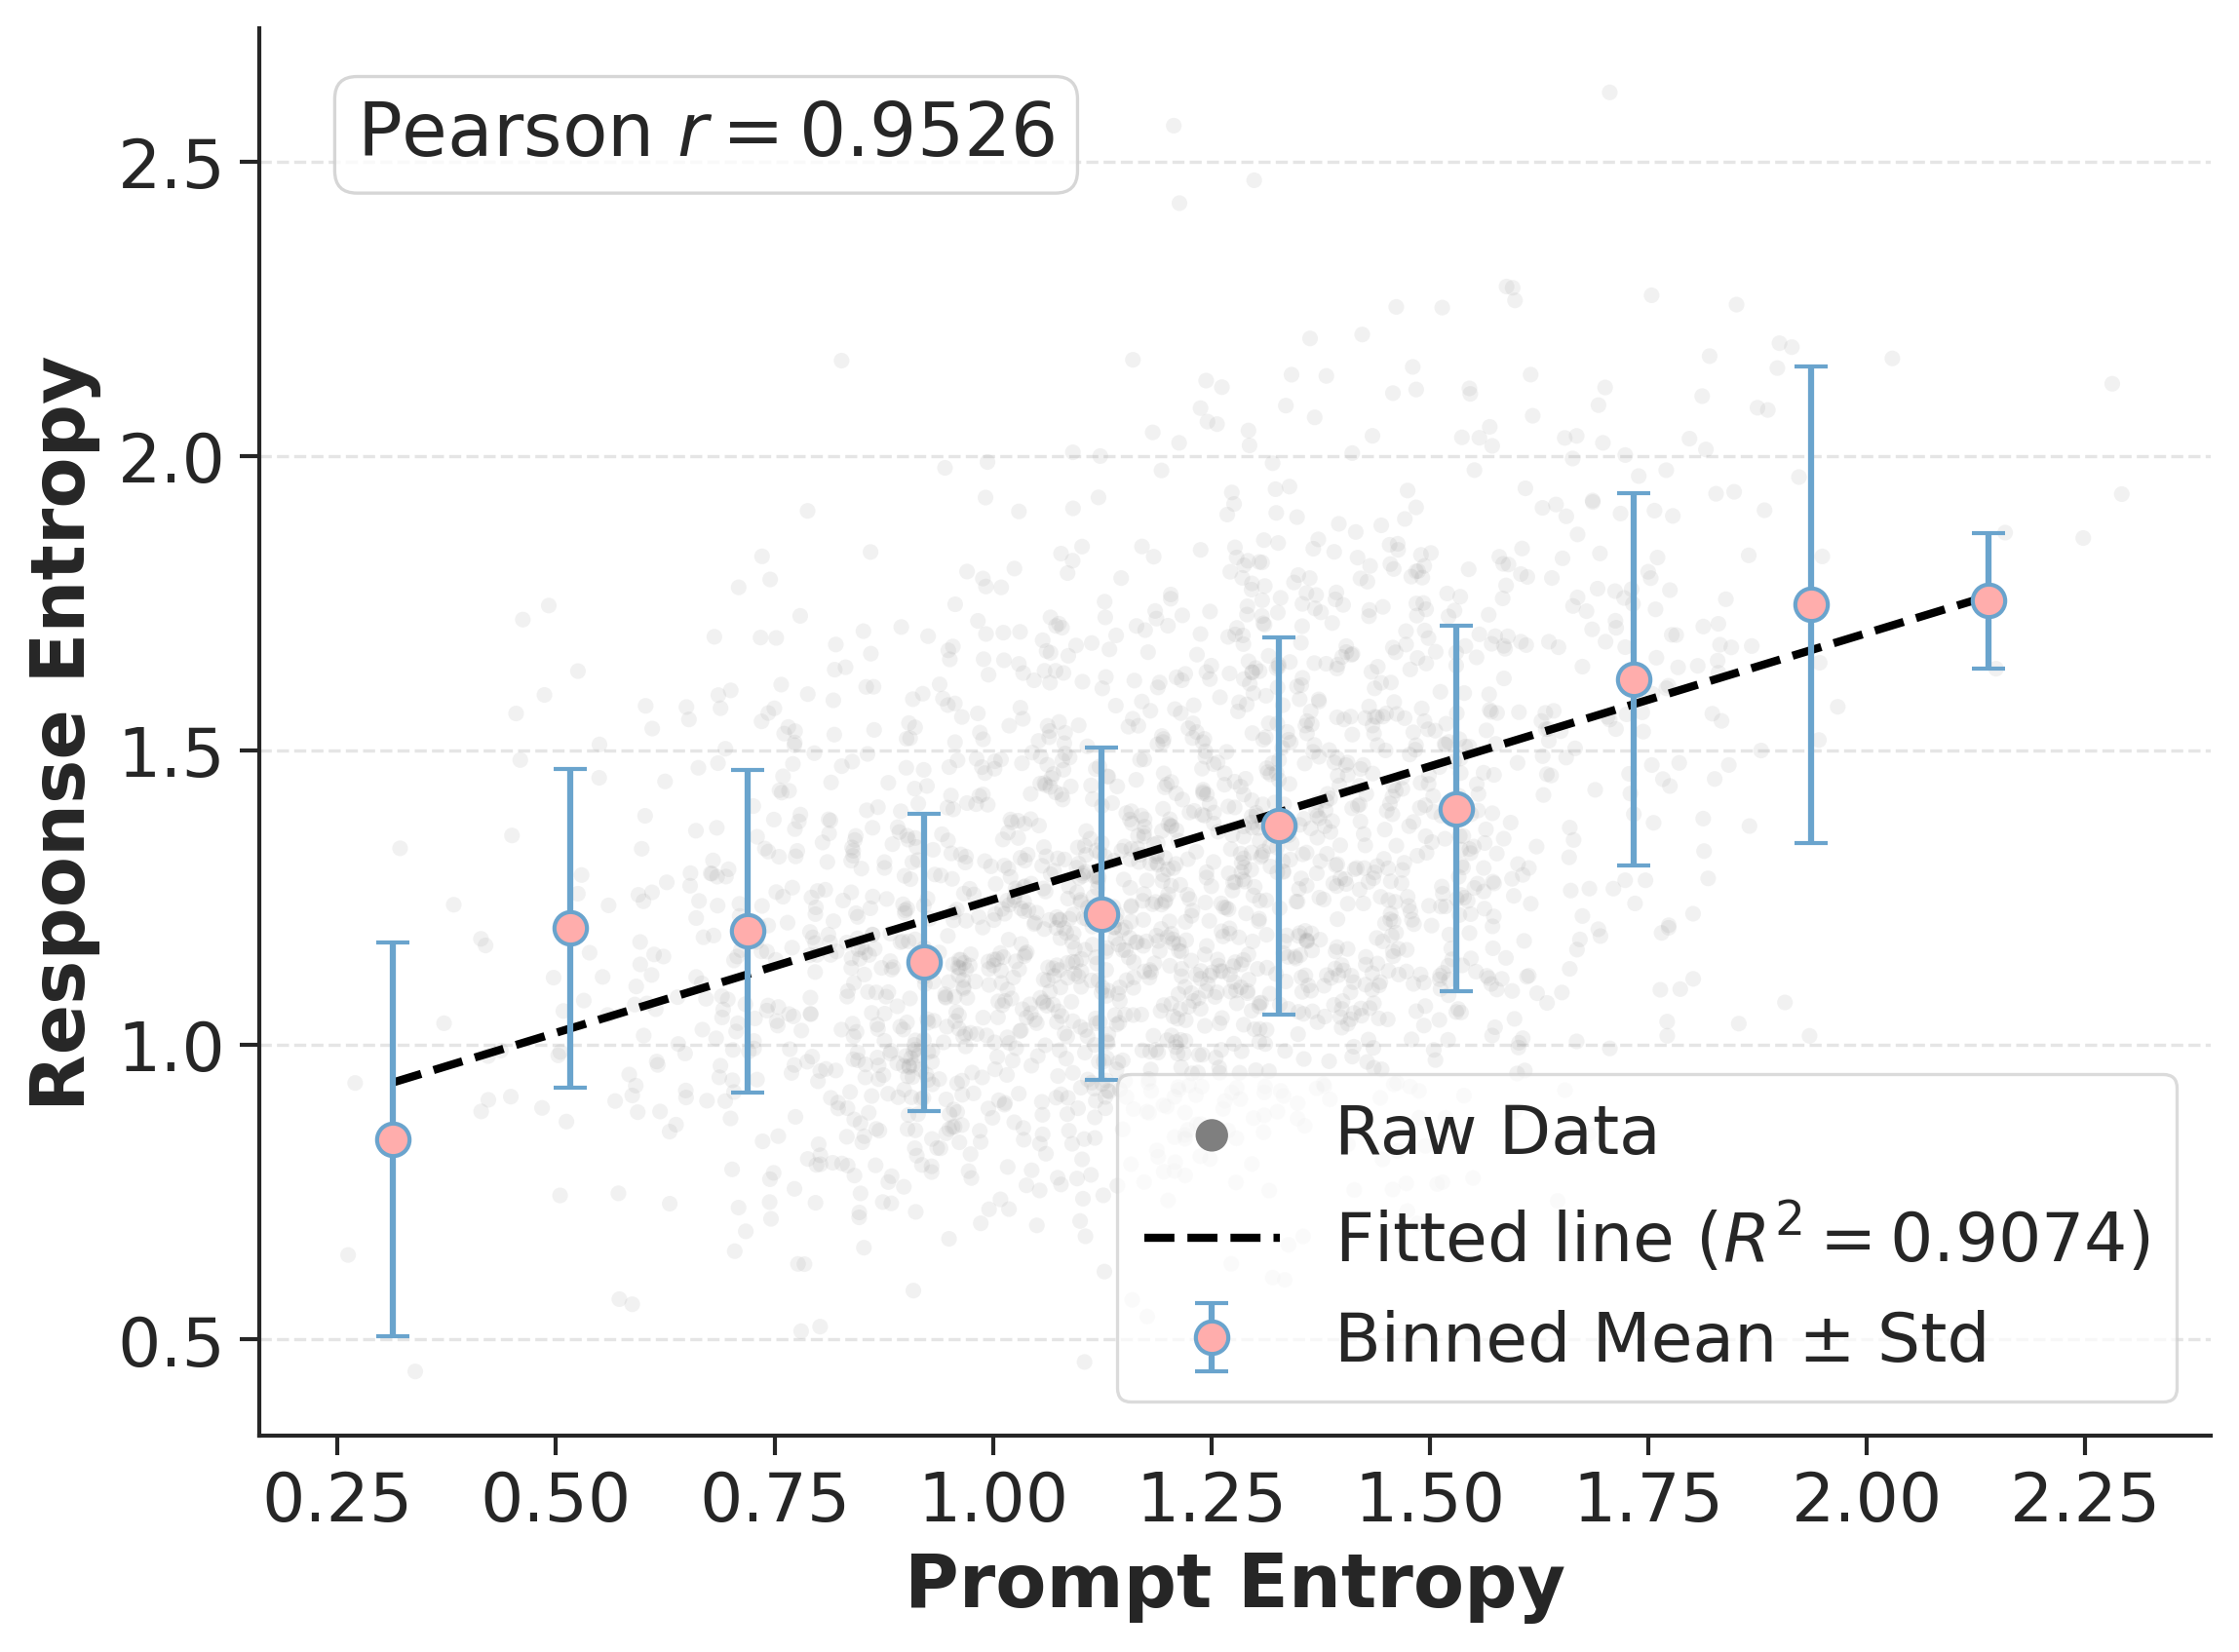
\includegraphics[width=\linewidth]{figures/appendix/binned_mean_respRatio10.png}
        \caption{$r=10\%$}
        \label{fig:respRatio10}
    \end{subfigure}
    \hfill
    \begin{subfigure}[b]{0.45\linewidth}
        \centering
        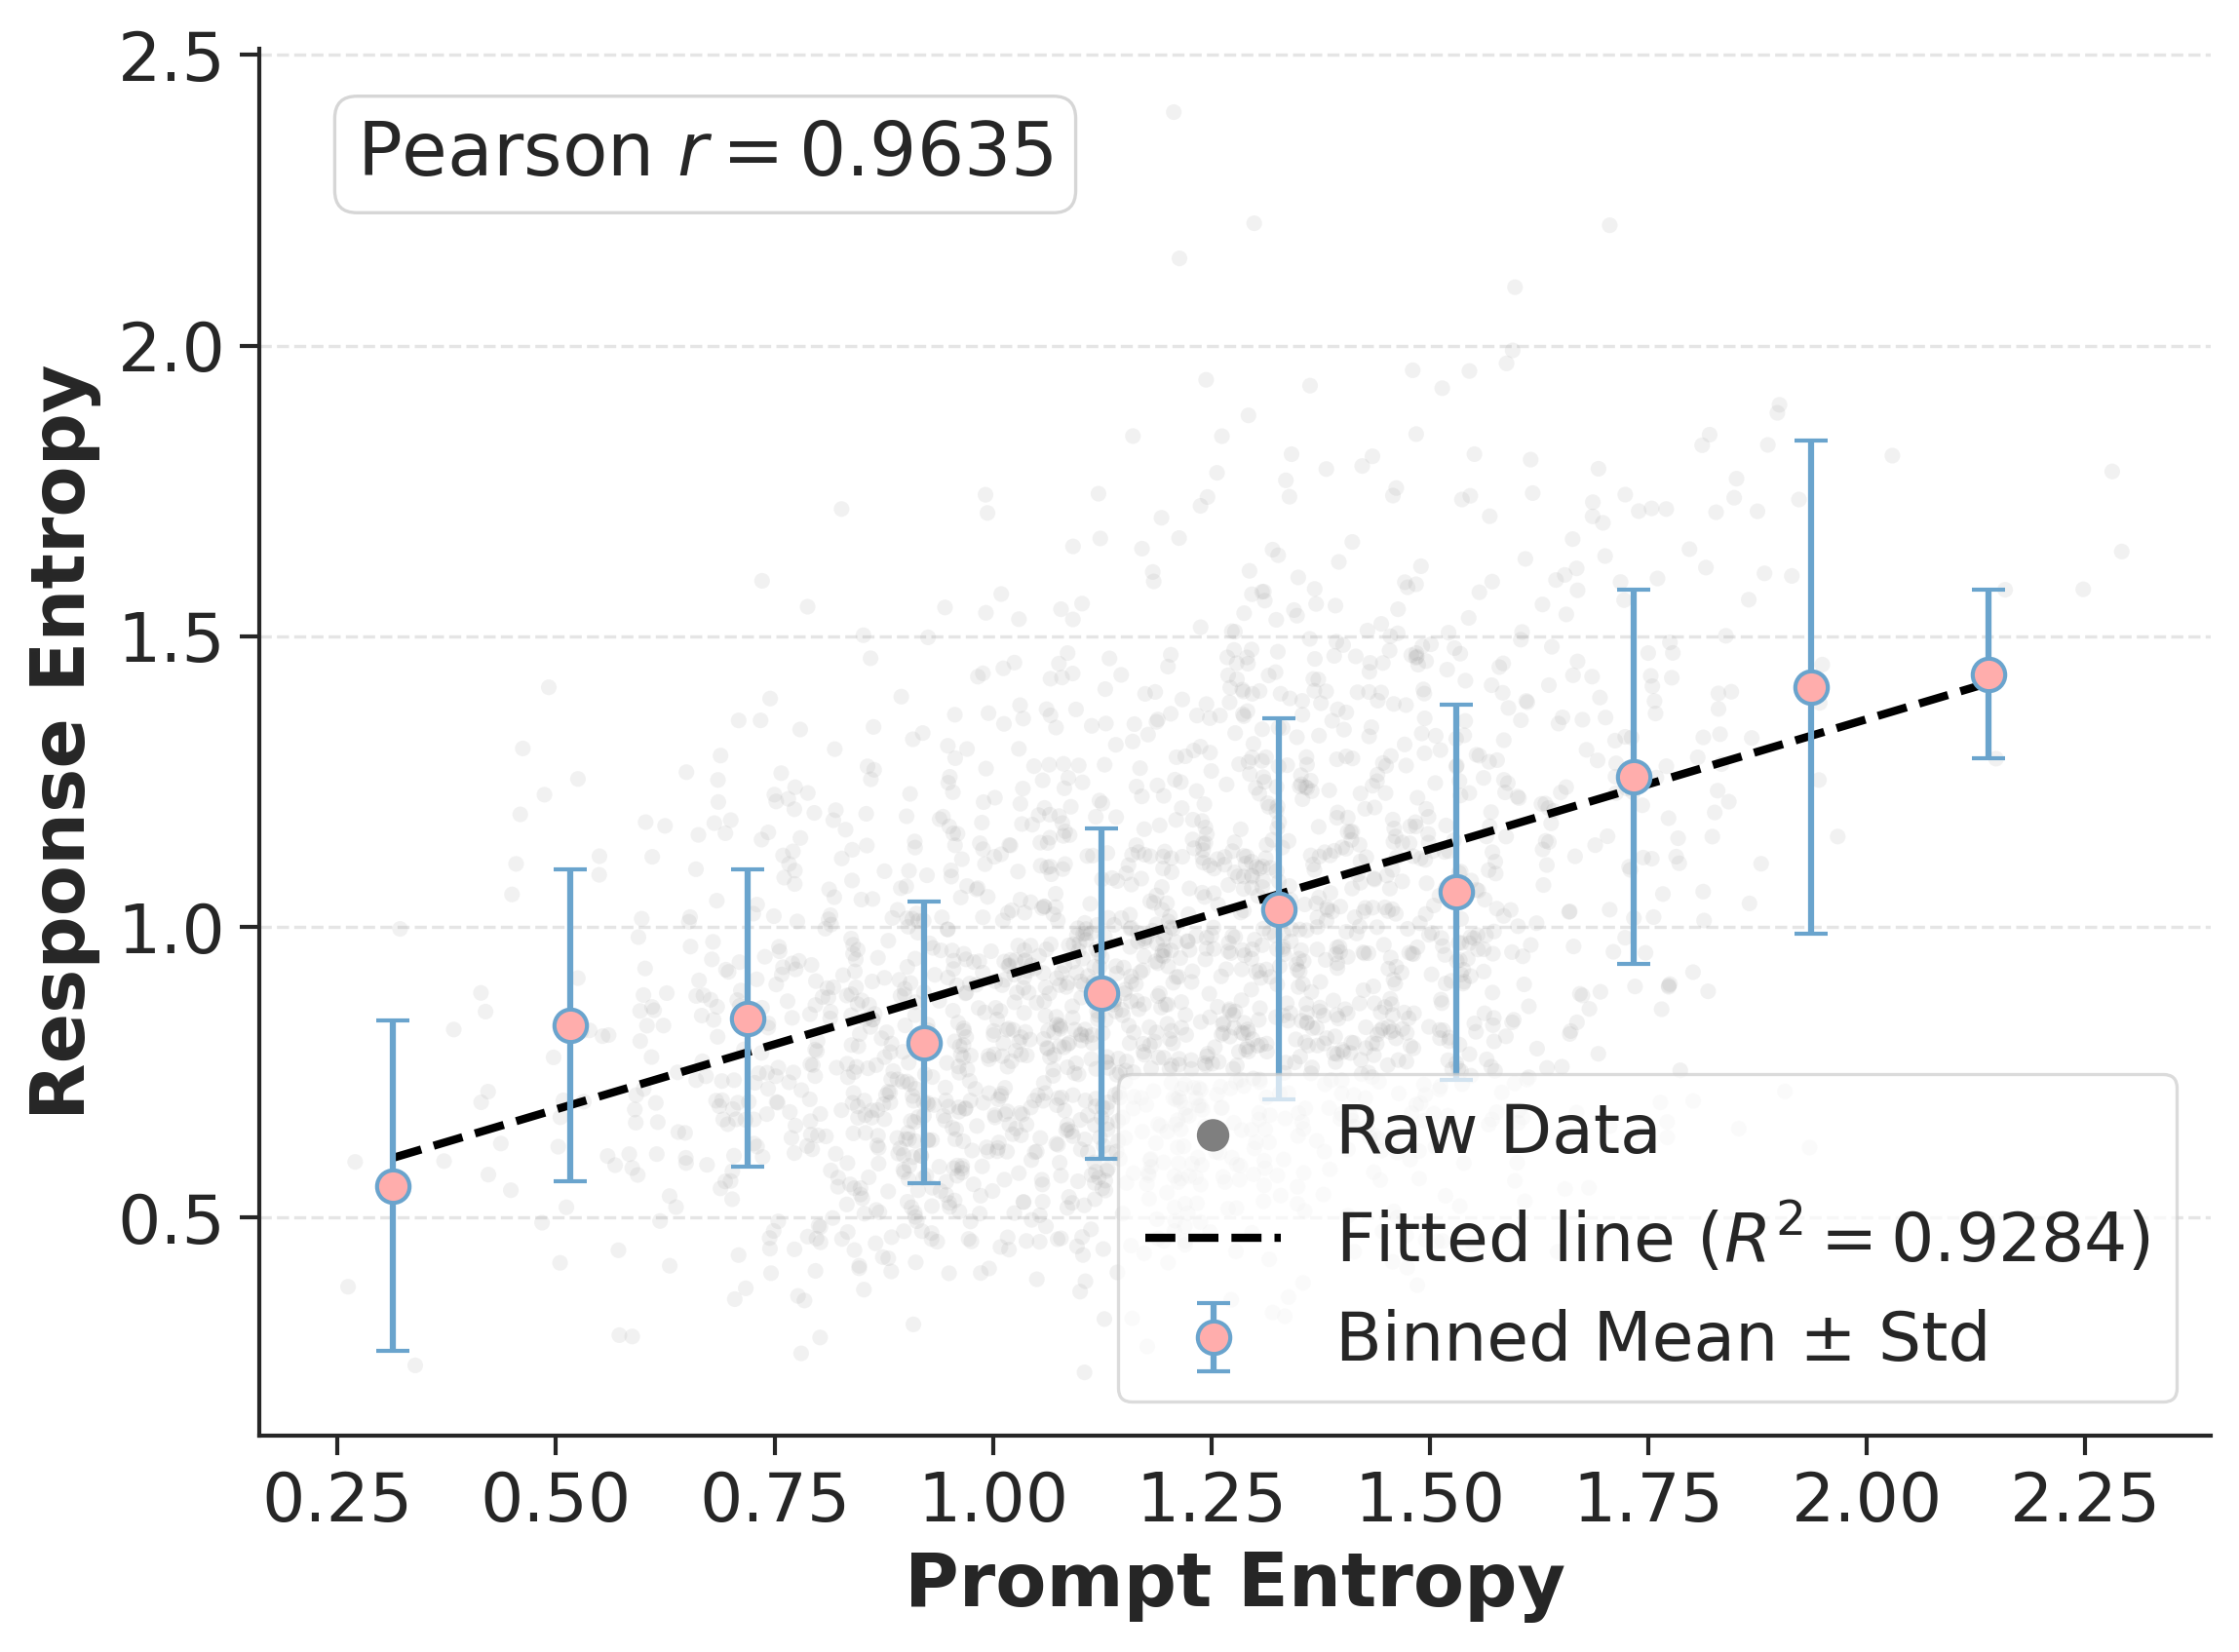
\includegraphics[width=\linewidth]{figures/appendix/binned_mean_respRatio20.png}
        \caption{$r=20\%$}
        \label{fig:respRatio20}
    \end{subfigure}

    \vspace{0.8em} % 行间距，可按版面微调

    % Row 2
    \begin{subfigure}[b]{0.45\linewidth}
        \centering
        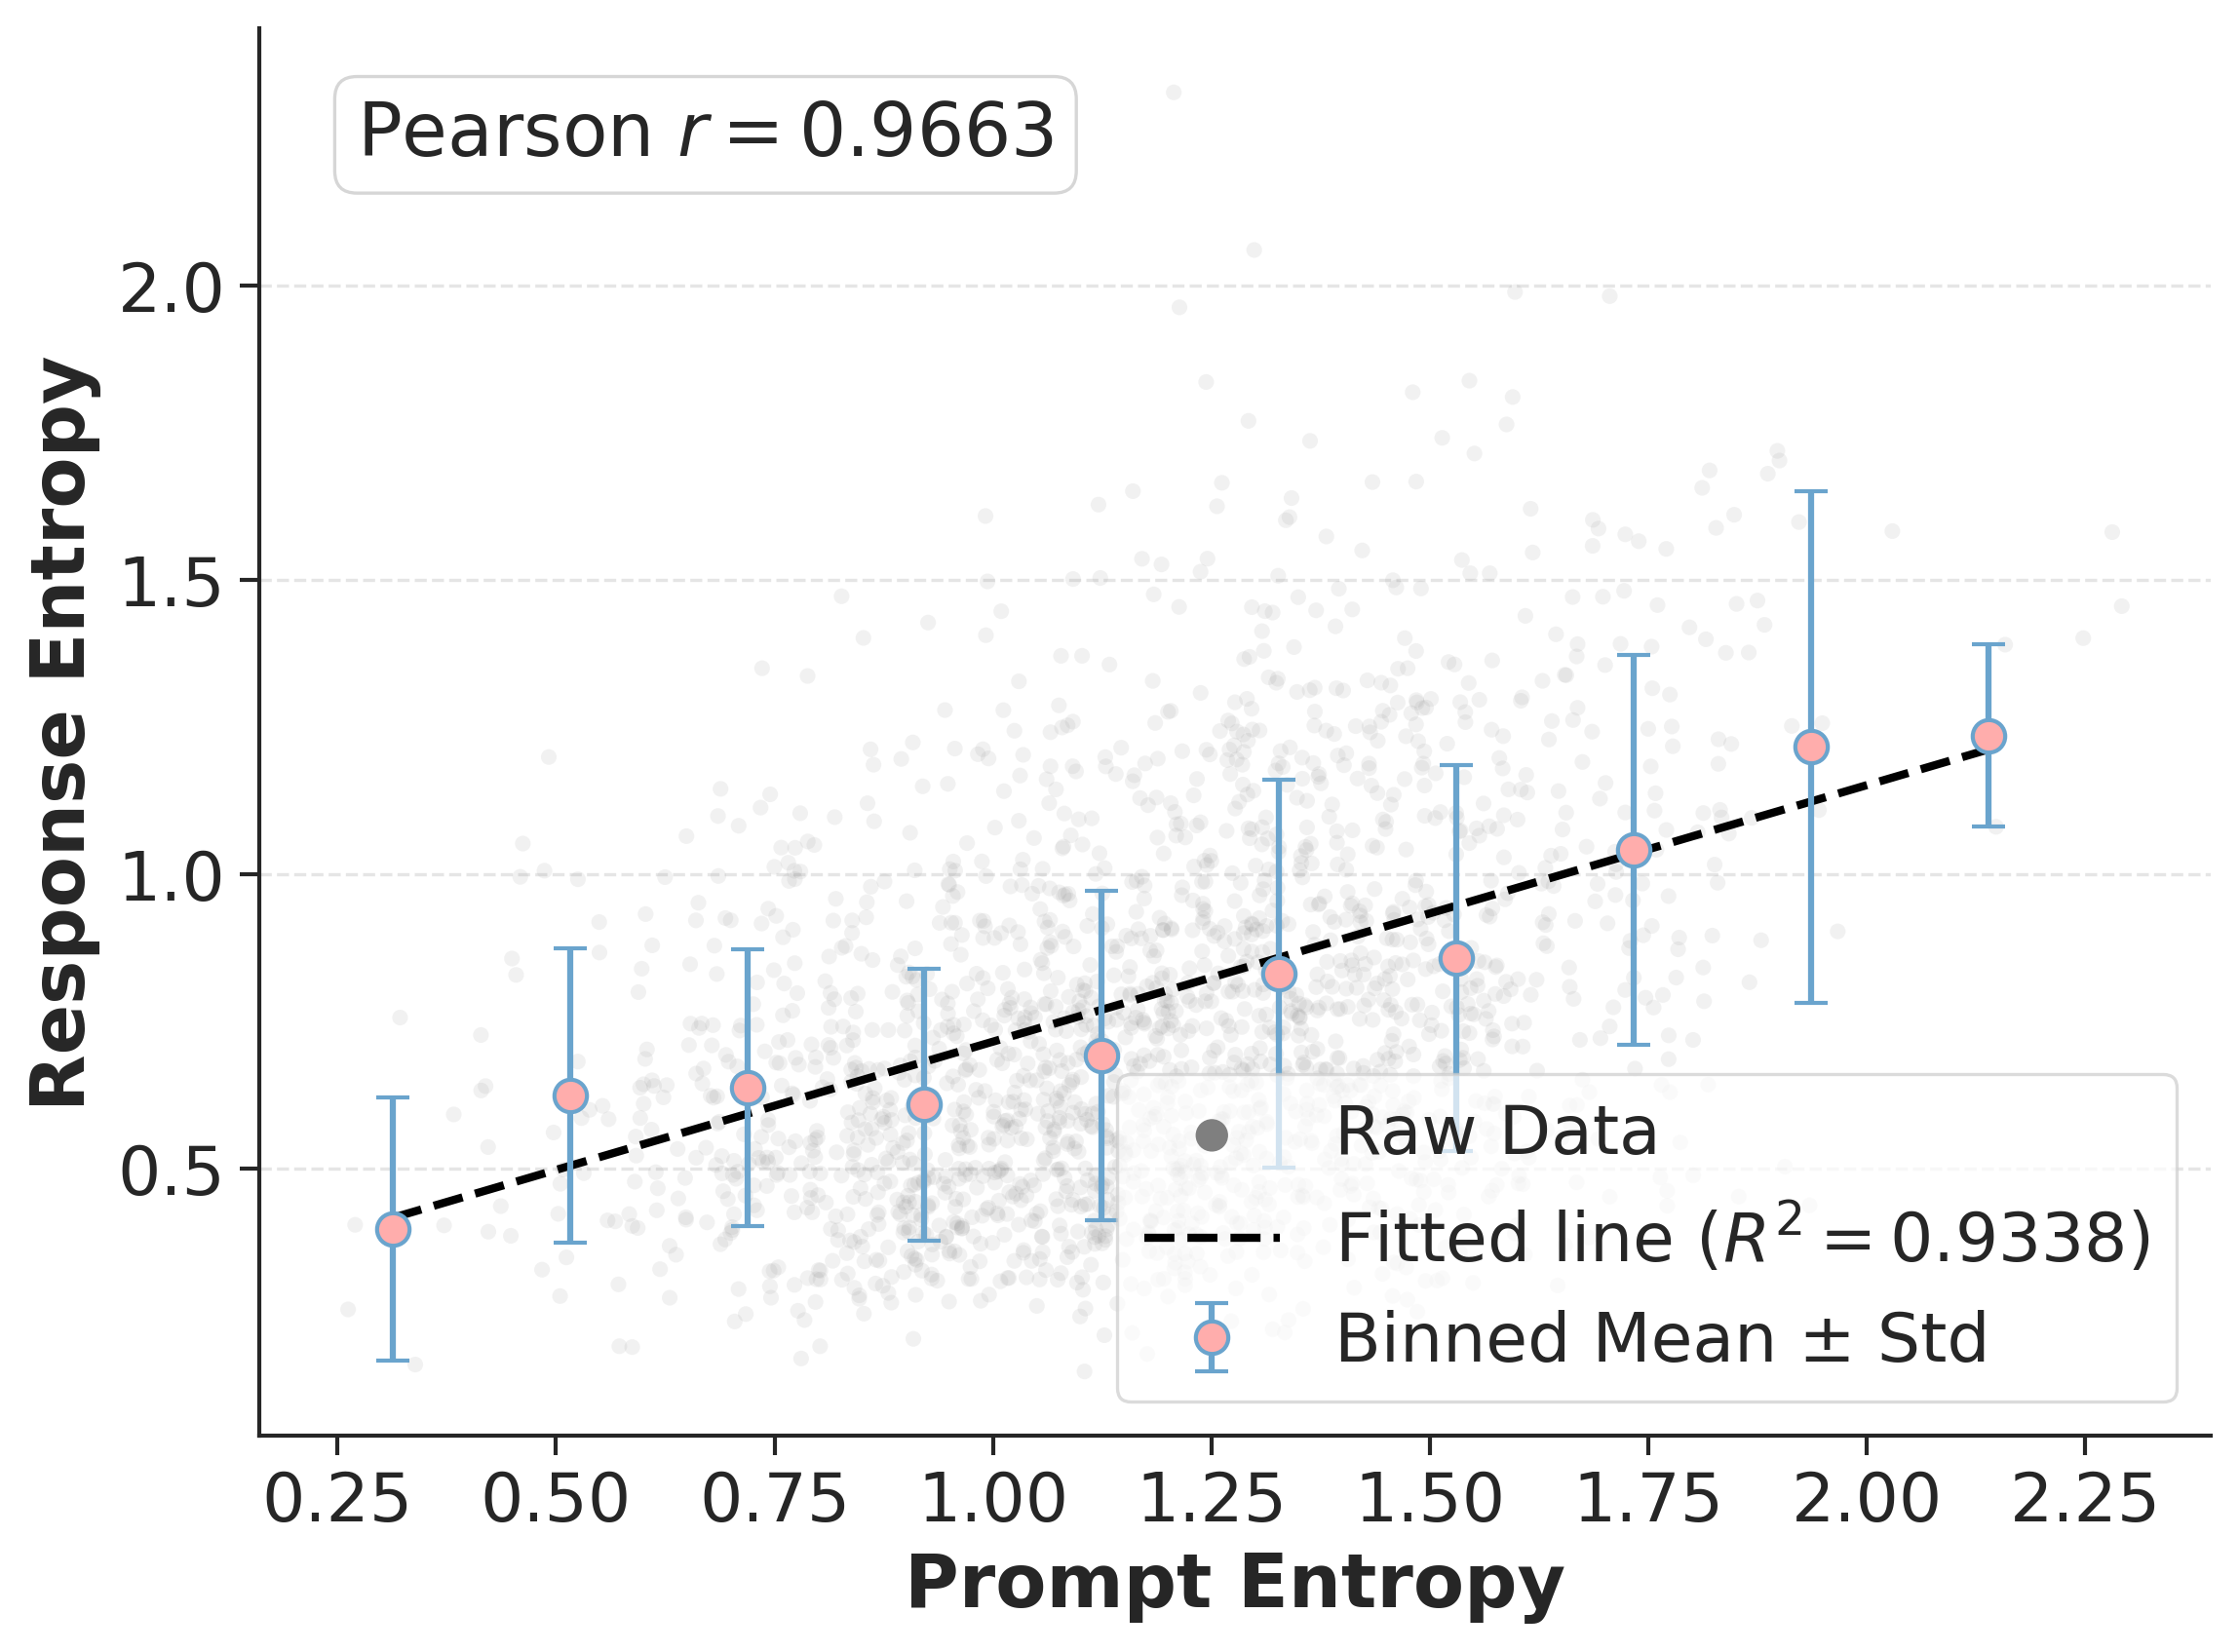
\includegraphics[width=\linewidth]{figures/appendix/binned_mean_respRatio30.png}
        \caption{$r=30\%$}
        \label{fig:respRatio30}
    \end{subfigure}
    \hfill
    \begin{subfigure}[b]{0.45\linewidth}
        \centering
        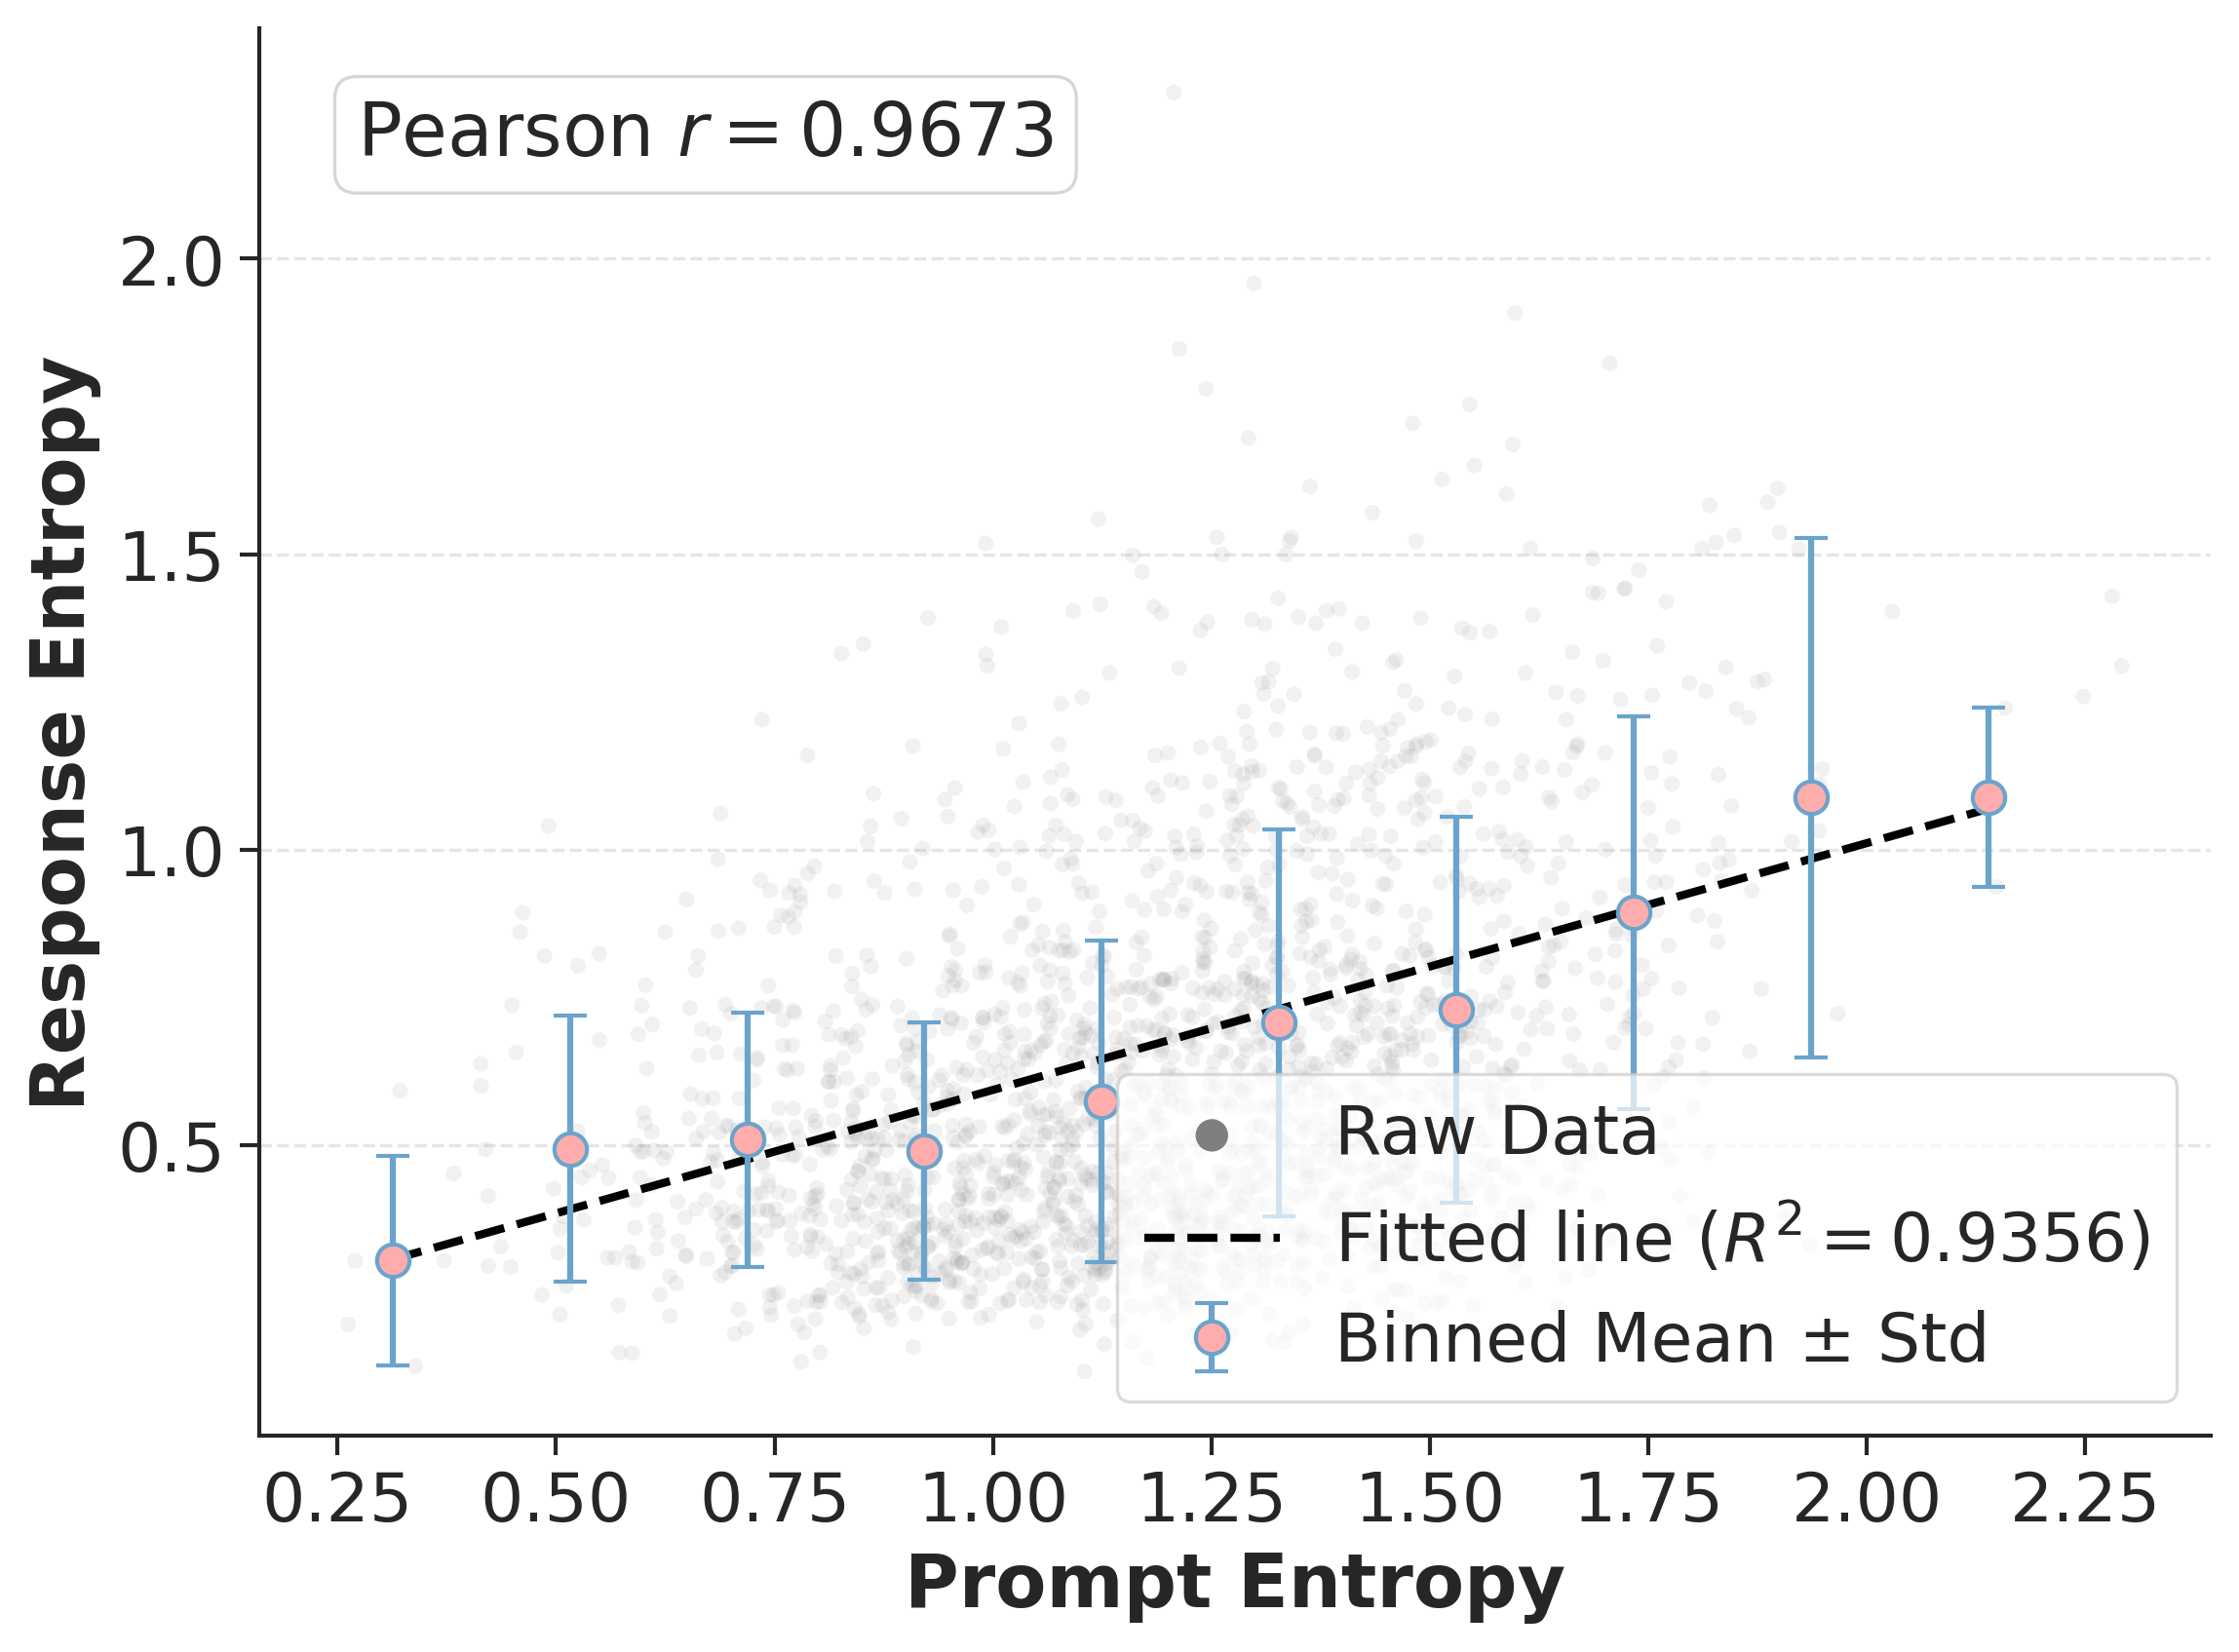
\includegraphics[width=\linewidth]{figures/appendix/binned_mean_respRatio40.png}
        \caption{$r=40\%$}
        \label{fig:respRatio40}
    \end{subfigure}
    
    \caption{Relationship between prompt entropy and response entropy computed over the top-$r\%$ tokens in the response distribution, sweeping $r\in\{10,20,30,40\}$. Each panel reports the binned mean trend under the corresponding ratio setting.}
    \label{fig:combined_results_appendix}
\end{figure}

\section{Additional Experiments}
\label{appendix-sec:additional-exp}
\subsection{Correlation Between Prompt Entropy and Response Entropy}

Building on the empirical validation of Assumption \ref{ass:propagation}, we conduct an additional robustness study by redefining the response entropy $S_{\mathrm{resp}}(x)$ as the entropy computed over only the top-$r\%$ tokens of the response distribution, sweeping $r \in \{10,20,30,40\}$. To suppress intrinsic decoding stochasticity, we follow the same binned-mean protocol on 2{,}048 prompts, binning by $S_{\mathrm{prompt}}(x)$ (proxied by $V(x)$) and averaging $S_{\mathrm{resp}}^{(r)}(x)$ within each bin. As shown in Figure~\ref{fig:combined_results_appendix}, the prompt--response relationship remains strongly linear across all ratios.
This indicates that the prompt--response entropy relationship is robust to this response-entropy definition, further supporting the bounded-noise linear approximation used in Assumption~\ref{ass:propagation}.
 





\subsection{Case Study}

To gain deeper insight into the behavior of our selective filtering algorithm, we analyze a case study based on prompts from the MATH dataset. 
We divide these prompts into four categories: Frequently Skipped Prompts (Easy), Frequently Skipped Prompts (Hard), Frequently Selected Prompts, and Prompts Frequently Selected by Stage 1 but Skipped by Stage 2.
We observe that frequently skipped easy prompts often involve simple computations or routine use of formulas, leading to high solution rates across sampled responses. In contrast, hard prompts that are often skipped tend to be too difficult for the model, leading to low or zero success across rollouts, limiting their value for training.
Frequently selected prompts tend to be moderately difficult, making consistent contributions to model learning. 
Furthermore, we analyze the prompts selected in stage 1 but filtered after stage 2. 
Most prompts are relatively easy, showing that the historical information is not reliable for filtering.



\begin{tcolorbox}[casestudy={Frequently Skipped Prompts (Easy)}]
1. \textbf{Question:} What is the value of $(2x + 5)^2$ when $x = 3$? \textbf{Solution:} 121.
\vspace{0.2cm}

2. \textbf{Question:} Solve for $x$: $5^{x + 4} = 125^x$?  
\textbf{Solution:} 21.
\vspace{0.2cm}

3. \textbf{Question:} A squirrel travels at a constant 4 miles per hour. How long does it take for this squirrel to travel 1 mile? Express your answer in minutes.  
\textbf{Solution:} 15.
\vspace{0.2cm}

4. \textbf{Question:} Evaluate $\text{log}_5 625$.  
\textbf{Solution:} 4.
\vspace{0.2cm}

5. \textbf{Question:} What value of $x$ will give the minimum value for $x^2- 10x + 24$? 
\textbf{Solution:} 5.
\end{tcolorbox}


\begin{tcolorbox}[casestudy={Frequently Skipped Prompts (Hard)}]
1. \textbf{Question:} Let $\triangle{PQR}$ be a right triangle with $PQ = 90$, $PR = 120$, and $QR = 150$. Let $C_{1}$ be the inscribed circle. Construct $\overline{ST}$ with $S$ on $\overline{PR}$ and $T$ on $\overline{QR}$, such that $\overline{ST}$ is perpendicular to $\overline{PR}$ and tangent to $C_{1}$. Construct $\overline{UV}$ with $U$ on $\overline{PQ}$ and $V$ on $\overline{QR}$ such that $\overline{UV}$ is perpendicular to $\overline{PQ}$ and tangent to $C_{1}$. Let $C_{2}$ be the inscribed circle of $\triangle{RST}$ and $C_{3}$ the inscribed circle of $\triangle{QUV}$. The distance between the centers of $C_{2}$ and $C_{3}$ can be written as $\sqrt {10n}$. What is $n$?
\textbf{Solution:} 725.
\vspace{0.2cm}

2. \textbf{Question:} Consider the region $A^{}_{}$ in the complex plane that consists of all points $z^{}_{}$ such that both $\frac{z^{}_{}}{40}$ and $\frac{40^{}_{}}{\overline{z}}$ have real and imaginary parts between $0^{}_{}$ and $1^{}_{}$, inclusive. Find the area of $A.$
\textbf{Solution:} $1200 - 200 \pi$.
\vspace{0.2cm}

3. \textbf{Question:} Ephram is growing $3$ different variants of radishes in a row of $13$ radishes total, but he forgot where he planted each radish variant and he can't tell what variant a radish is before he picks it. Ephram knows that he planted at least one of each radish variant, and all radishes of one variant will form a consecutive string, with all such possibilities having an equal chance of occurring. He wants to pick three radishes to bring to the farmers market, and wants them to all be of different variants. Given that he uses optimal strategy, the probability that he achieves this can be expressed as $\frac{m}{n}$, where $m$ and $n$ are relatively prime positive integers. Find $m+n$.  
\textbf{Solution:} 17.
\vspace{0.2cm}

4. \textbf{Question:} There are 1000 rooms in a row along a long corridor. Initially, the first room contains 1000 people, and the remaining rooms are empty. Each minute, the following happens: for each room containing more than one person, someone in that room decides it is too crowded and moves to the next room. All these movements are simultaneous (so nobody moves more than once within a minute). After one hour, how many different rooms will have people in them?  
\textbf{Solution:} 31.
\vspace{0.2cm}

5. \textbf{Question:} A regular hexagon has side length \(6\). Congruent arcs with radius \(3\) are drawn with the center at each of the vertices, creating circular sectors as shown. The region inside the hexagon but outside the sectors is shaded as shown. The original answer is in the form \(a\sqrt{b}-c\pi\). Please find the value of a + b + c.
\textbf{Solution:} 75.
\end{tcolorbox}


\begin{tcolorbox}[casestudy={Frequently Selected Prompts After Stage 2}]
1. \textbf{Question:} Let $z$ be a complex number such that
\[|z - 12| + |z - 5i| = 13.\]
Find the smallest possible value of $|z|.$ \textbf{Solution:} $\frac{60}{13}$.
\vspace{0.2cm}

2. \textbf{Question:} Find all real solutions to $x^4+(2-x)^4=34$.  Enter all the solutions, separated by commas.  
\textbf{Solution:} $1 + \sqrt{2}, 1 - \sqrt{2}$.
\vspace{0.2cm}

3. \textbf{Question:} Let b be a real number randomly selected from the interval $[-17,17]$. Then, m and n are two relatively prime positive integers such that m\/n is the probability that the equation $x^4+25b^2=(4b^2-10b)x^2$ has $\textit{at least}$ two distinct real solutions. Find the value of $m+n$. 
\textbf{Solution:} 63.
\vspace{0.2cm}

4. \textbf{Question:} Let $a,$ $b,$ $c,$ $d$ be real numbers such that\[\\frac{(a - b)(c - d)}{(b - c)(d - a)} = \\frac{2}{5}.\]Find the sum of all possible values of\[\frac{(a - c)(b - d)}{(a - b)(c - d)}.\]  
\textbf{Solution:} $-\frac{3}{2}$.
\vspace{0.2cm}

5. \textbf{Question:} The function $f$, defined on the set of ordered pairs of positive integers, satisfies the following properties: 
\begin{align*}  f(x,x) &=x, \\  f(x,y) &=f(y,x), \quad \text{and} \\ (x + y) f(x,y) &= yf(x,x + y).  
\end{align*}
Calculate $f(14,52)$. 
\textbf{Solution:} 364.
\end{tcolorbox}


\begin{tcolorbox}[casestudy={Prompts Frequently Selected by Stage 1 but Skipped by Stage 2}]
1. \textbf{Question:} A polynomial with integer coefficients is of the form
\[9x^4 + a_3 x^3 + a_2 x^2 + a_1 x + 15 = 0.\]
Find the number of different possible rational roots of this polynomial.
\textbf{Solution:} 16.
\vspace{0.2cm}

2. \textbf{Question:} When an integer is divided by 15, the remainder is 7. Find the sum of the remainders when the same integer is divided by 3 and by 5.  
\textbf{Solution:} 3.
\vspace{0.2cm}

3. \textbf{Question:} Find the number of positive divisors of 2002.  
\textbf{Solution:} 16.
\vspace{0.2cm}

4. \textbf{Question:} What is the base five product of the numbers $121_{5}$ and $11_{5}$?
\textbf{Solution:} 1331.
\vspace{0.2cm}

5. \textbf{Question:} If $\sin x = 3 \cos x,$ then what is $\sin x \cos x$ 
\textbf{Solution:} $\frac{3}{10}$.
\end{tcolorbox}

\begin{algorithm}[t]
\caption{Training Iteration in HIVE}
\label{alg:hive-training}
\begin{algorithmic}[1]
    \REQUIRE Dataset $\mathcal{D}$; Historical trace $\mathcal{T}$; Target training batch size $B_{\text{t}}$; Group size $G$; Base exploration probability $p_{e,easy}$, $p_{e,hard}$; Step size $\Delta p$; Target zero-var ratio $\alpha$.
    
    \STATE $\mathcal{D}_{cand} \gets \emptyset$
    \STATE $n_{easy}, n_{hard}, n_{total} \gets 0, 0, 0$
    
    \STATE \textcolor{gray}{\textit{\# Stage 1: History-Informed Selection}}
    \REPEAT
        \STATE $\{x_i\} \gets \text{Sample raw prompts from } \mathcal{D}$
        \FOR{each $x_i$ in batch}
            \STATE Retrieve zero-var count $z_i$, zero-var type, and history entropy $H_i$ from $\mathcal{T}$
            \STATE Choose $p_e \gets p_{e,easy}$, $p_{e,hard}$, or the default $p_e$ according to the zero-var type
            \STATE $P_{Rew} \gets p_e^{z_i}; \quad P_{Ent} \gets \text{Normalize}(H_i)$
            \STATE $P_{select} \gets \lambda P_{Rew} + (1-\lambda) P_{Ent}$
            
            \IF{$\text{Bernoulli}(P_{select}) = 1$}
                \STATE $\mathcal{D}_{cand} \gets \mathcal{D}_{cand} \cup \{x_i\}$
            \ENDIF
        \ENDFOR
    % \UNTIL{$|\mathcal{D}_{cand}| \geq 2 \cdot B_{\text{t}}$}
    \UNTIL{$|\mathcal{D}_{cand}| \geq B_{\mathrm{cand}}$ \quad\textcolor{gray}{\textit{\# $B_{\mathrm{cand}}{=}1.5\,B_{\mathrm{t}}$ in our experiments; see Appendix~\ref{appendix-subsec:hive-hyperparams}}}}

    \STATE \textcolor{gray}{\textit{\# Stage 2: Online-Verified Selection}} %(Deterministic Gate)
    \STATE Calculate prompt entropy $V(x)$ for all $x \in \mathcal{D}_{cand}$
    \STATE $\gamma \gets \text{median}(\{V(x) \mid x \in \mathcal{D}_{cand}\})$
    \STATE $\mathcal{D}_{final} \gets \{x \in \mathcal{D}_{cand} \mid V(x) \geq \gamma\}$

    \STATE \textcolor{gray}{\textit{\# Rollout Phase}}
    \STATE $\{x_i, r_i\} \gets \text{Generate } G \text{ rollouts for each } x \in \mathcal{D}_{final}$

    \STATE \textcolor{gray}{\textit{\# GRPO Training}}
    \STATE Update policy model $\pi_\theta$ using GRPO on $\{x_i, r_i\}$
    
    \STATE \textcolor{gray}{\textit{\# History Update \& Statistics}}
    \STATE Update $\mathcal{T}$ with new rewards and response entropies
    \STATE $n_{total} \gets |\mathcal{D}_{final}|$
    \STATE $n_{easy} \gets \text{count\_zero\_var}(\text{easy\_subset}); \quad n_{hard} \gets \text{count\_zero\_var}(\text{hard\_subset})$

    \STATE \textcolor{gray}{\textit{\# Adaptive Exploration Adjustment}}
    \FOR{type $\in \{easy, hard\}$}
        \IF{$n_{\text{type}} / n_{\text{total}} > \alpha$}
            \STATE $p_{e,\text{type}} \gets p_{e,\text{type}} - \Delta p$
        \ELSE
            \STATE $p_{e,\text{type}} \gets p_{e,\text{type}} + \Delta p$
        \ENDIF
    \ENDFOR


\end{algorithmic}
\end{algorithm}

\section{{Algorithm}}
\label{appendix-sec:alg}

The HIVE training procedure is illustrated in Algorithm~\ref{alg:hive-training}. 
The process begins with \textbf{History-Informed Selection}, where the method iteratively samples raw prompts from the dataset $\mathcal{D}$. 
For each sampled prompt, we retrieve its historical metadata, consisting of the consecutive zero-variance counts $z_i$ and the historical response entropy $H_i$. These metrics are combined into a selection probability $P_{select}$ using a weighted combination of reward decay and entropy normalization. We employ Bernoulli sampling to accumulate a candidate pool $\mathcal{D}_{cand}$ until its size reaches twice the target training batch size (i.e., $2 \cdot B_t$). This $2\times$ oversampling strategy is a prerequisite for the subsequent median-based truncation, ensuring the final batch size aligns with the target computational budget.

Once the candidate pool is populated, the flow transitions to \textbf{Online-Verified Selection}, a deterministic gatekeeper grounded in the model's current state. For every candidate in $\mathcal{D}_{cand}$, we compute the prompt-side entropy $V(x)$ via a single efficient forward pass. To adaptively identify the current learning edge, we calculate the median entropy $\gamma = \text{median}(\{V(x)\})$ of the accumulated pool. A strict filter is then applied to retain only prompts where $V(x) \geq \gamma$. This step effectively discards the bottom 50\% of samples with low uncertainty, yielding a final high-utility batch $\mathcal{D}_{final}$.

% With the filtered batch established, the method proceeds to the normal \textbf{Rollout and Policy Update} phase, which is identical to the GRPO algorithm. 
% After training finishes, the resulting rewards and response entropies are immediately written back to the historical trace $\mathcal{T}$ to update the metadata for future iterations. 
With the filtered batch established, the method proceeds to the normal \textbf{Rollout and Policy Update} phase, which is identical to the GRPO algorithm.
After training finishes, the resulting rewards and response entropies are immediately written back to the historical trace $\mathcal{T}$ to update the metadata for future iterations.

A complete list of every selector hyperparameter (including $\lambda$, $\alpha$, $\Delta p$, $\epsilon_p$, $p_{\min}/p_{\max}$, $k_{\mathrm{keep}}$, $k_{\mathrm{off}}$, the trace and unseen-prompt initialization, and the exact batch-sizing protocol that produces a $B_{\mathrm{t}}$-prompt GRPO update) is provided in Appendix~\ref{appendix-subsec:hive-hyperparams}.

\section{Asset Licenses}
% \paragraph{.}
\label{sec:asset-licenses}
We use publicly available models, datasets, and software frameworks. 
Qwen2.5-Math, Qwen3, Llama3.2, DeepSeek-R1-Distill, DAPO+MATH, Open-R1, verl, and vLLM are used according to their original licenses and terms.  Table~\ref{tab:assets} summarizes the source and license information.

\begin{table}[h]
\centering
\caption{Sources and licenses of publicly available assets used in this work.}
\label{tab:assets}
\resizebox{\columnwidth}{!}{%
\begin{tabular}{llll}
\toprule
\textbf{Asset} & \textbf{Type} & \textbf{Source} & \textbf{License} \\
\midrule
Qwen2.5-Math        & Model     & huggingface.co/Qwen               & Apache 2.0 \\
Qwen3               & Model     & huggingface.co/Qwen               & Apache 2.0 \\
Llama-3.2           & Model     & huggingface.co/meta-llama         & Llama 3.2 Community \\
DeepSeek-R1-Distill & Model     & huggingface.co/deepseek-ai        & MIT \\
DAPO-Math-17k       & Dataset   & github.com/BytedTsinghua-SIA/DAPO & Apache 2.0 \\
MATH                & Dataset   & github.com/hendrycks/math         & MIT \\
Open-R1             & Framework & github.com/huggingface/open-r1    & Apache 2.0 \\
verl                & Framework & github.com/volcengine/verl        & Apache 2.0 \\
vLLM                & Framework & github.com/vllm-project/vllm      & Apache 2.0 \\
\bottomrule
\end{tabular}}
\end{table}


\newpage
\input{checklist}

\end{document}
